% docx2tex 1.7.1 --- ``Just out of this Word.'' 
% 
% docx2tex is Open Source and  
% you can download it on GitHub: 
% https://github.com/transpect/docx2tex 
%  
\documentclass{scrbook} 
\usepackage[T1]{fontenc} 
\usepackage[utf8]{inputenc} 
\usepackage{graphicx}
\usepackage{hyperref} 
\usepackage{multirow} 
\usepackage{tabularx} 
\usepackage{color} 
\usepackage{textcomp} 
\usepackage{tipa}
\usepackage{amsmath} 
\usepackage{amssymb} 
\usepackage{amsfonts} 
\usepackage{amsxtra} 
\usepackage{wasysym} 
\usepackage{isomath} 
\usepackage{mathtools} 
\usepackage{txfonts} 
\usepackage{upgreek} 
\usepackage{enumerate} 
\usepackage{tensor} 
\usepackage{pifont} 
\usepackage{ulem} 
\usepackage{xfrac} 
\usepackage{soul}
\usepackage{arydshln} 
\usepackage[english,dutch]{babel}
\definecolor{color-1}{rgb}{0.27,0.33,0.42}
\definecolor{color-2}{rgb}{0.18,0.33,0.59}

\begin{document}
\textbf{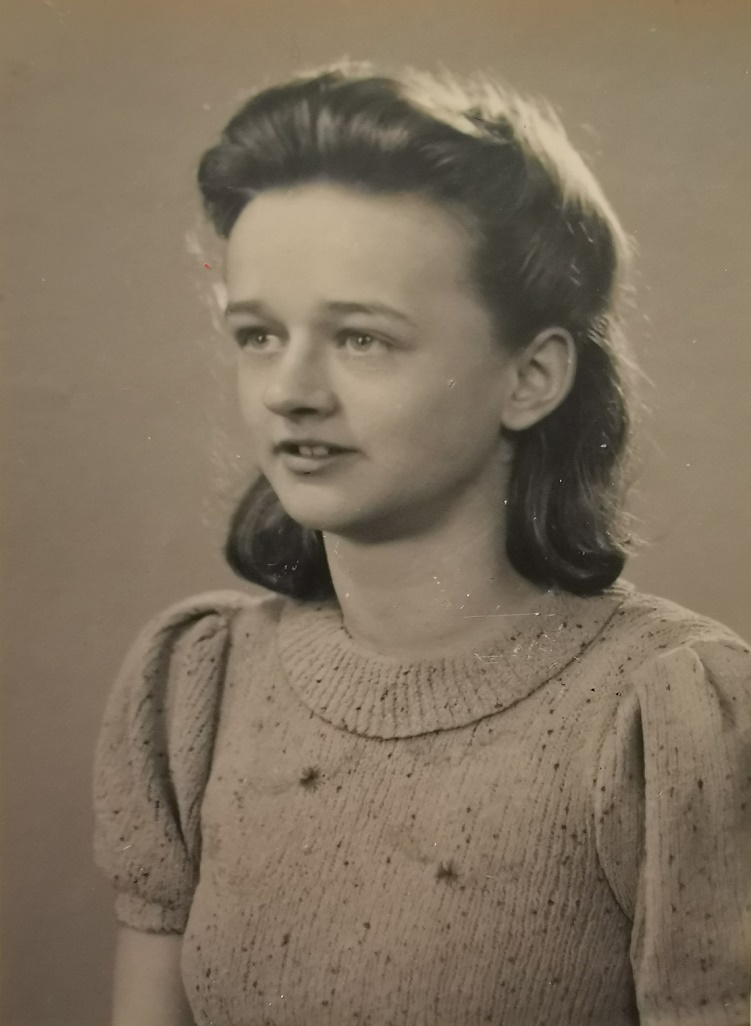
\includegraphics[height=0.5\textheight]{boek_Tine_Blom.docx.tmp/word/media/image1.jpeg}}

\textbf{Inhoudsopgave}

\tableofcontents

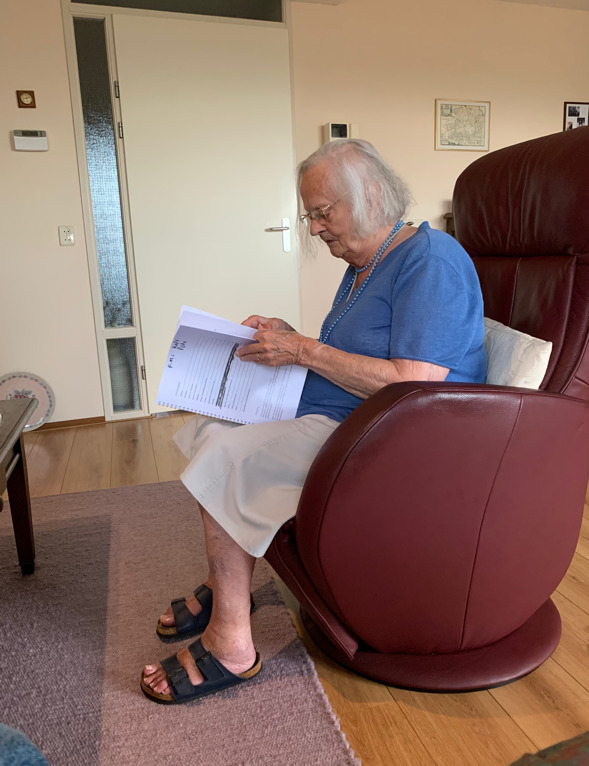
\includegraphics[width=1\textwidth]{boek_Tine_Blom.docx.tmp/word/media/image2.jpg}

\section{Inleiding}

In dit boek vertel ik, Tine de Booij, over mijn leven.

Het boek is opgebouwd uit interviews door mijn dochters Jacqueline en Yvonne en door mijn kleinkinderen Lisa, Anneflore en Dorus. Timon heeft de lay-out afgemaakt. En ik heb de eindcontrole gedaan.

Voor ons allemaal bijzonder om zo samen in het verleden te graven.

Af en toe leek het wel een officieel interview.

Het leidde ook tot mooie gesprekken over dingen waar we het nooit over hadden gehad.

Veel leesplezier!

\chapter{\label{ref-002}Oudkarspel}

Ik ben op 20 februari 1928 geboren. We zijn alle drie thuis geboren met hulp van de vroedvrouw. Bert was van 1924 en Kees van 1930. Ik zat er tussenin.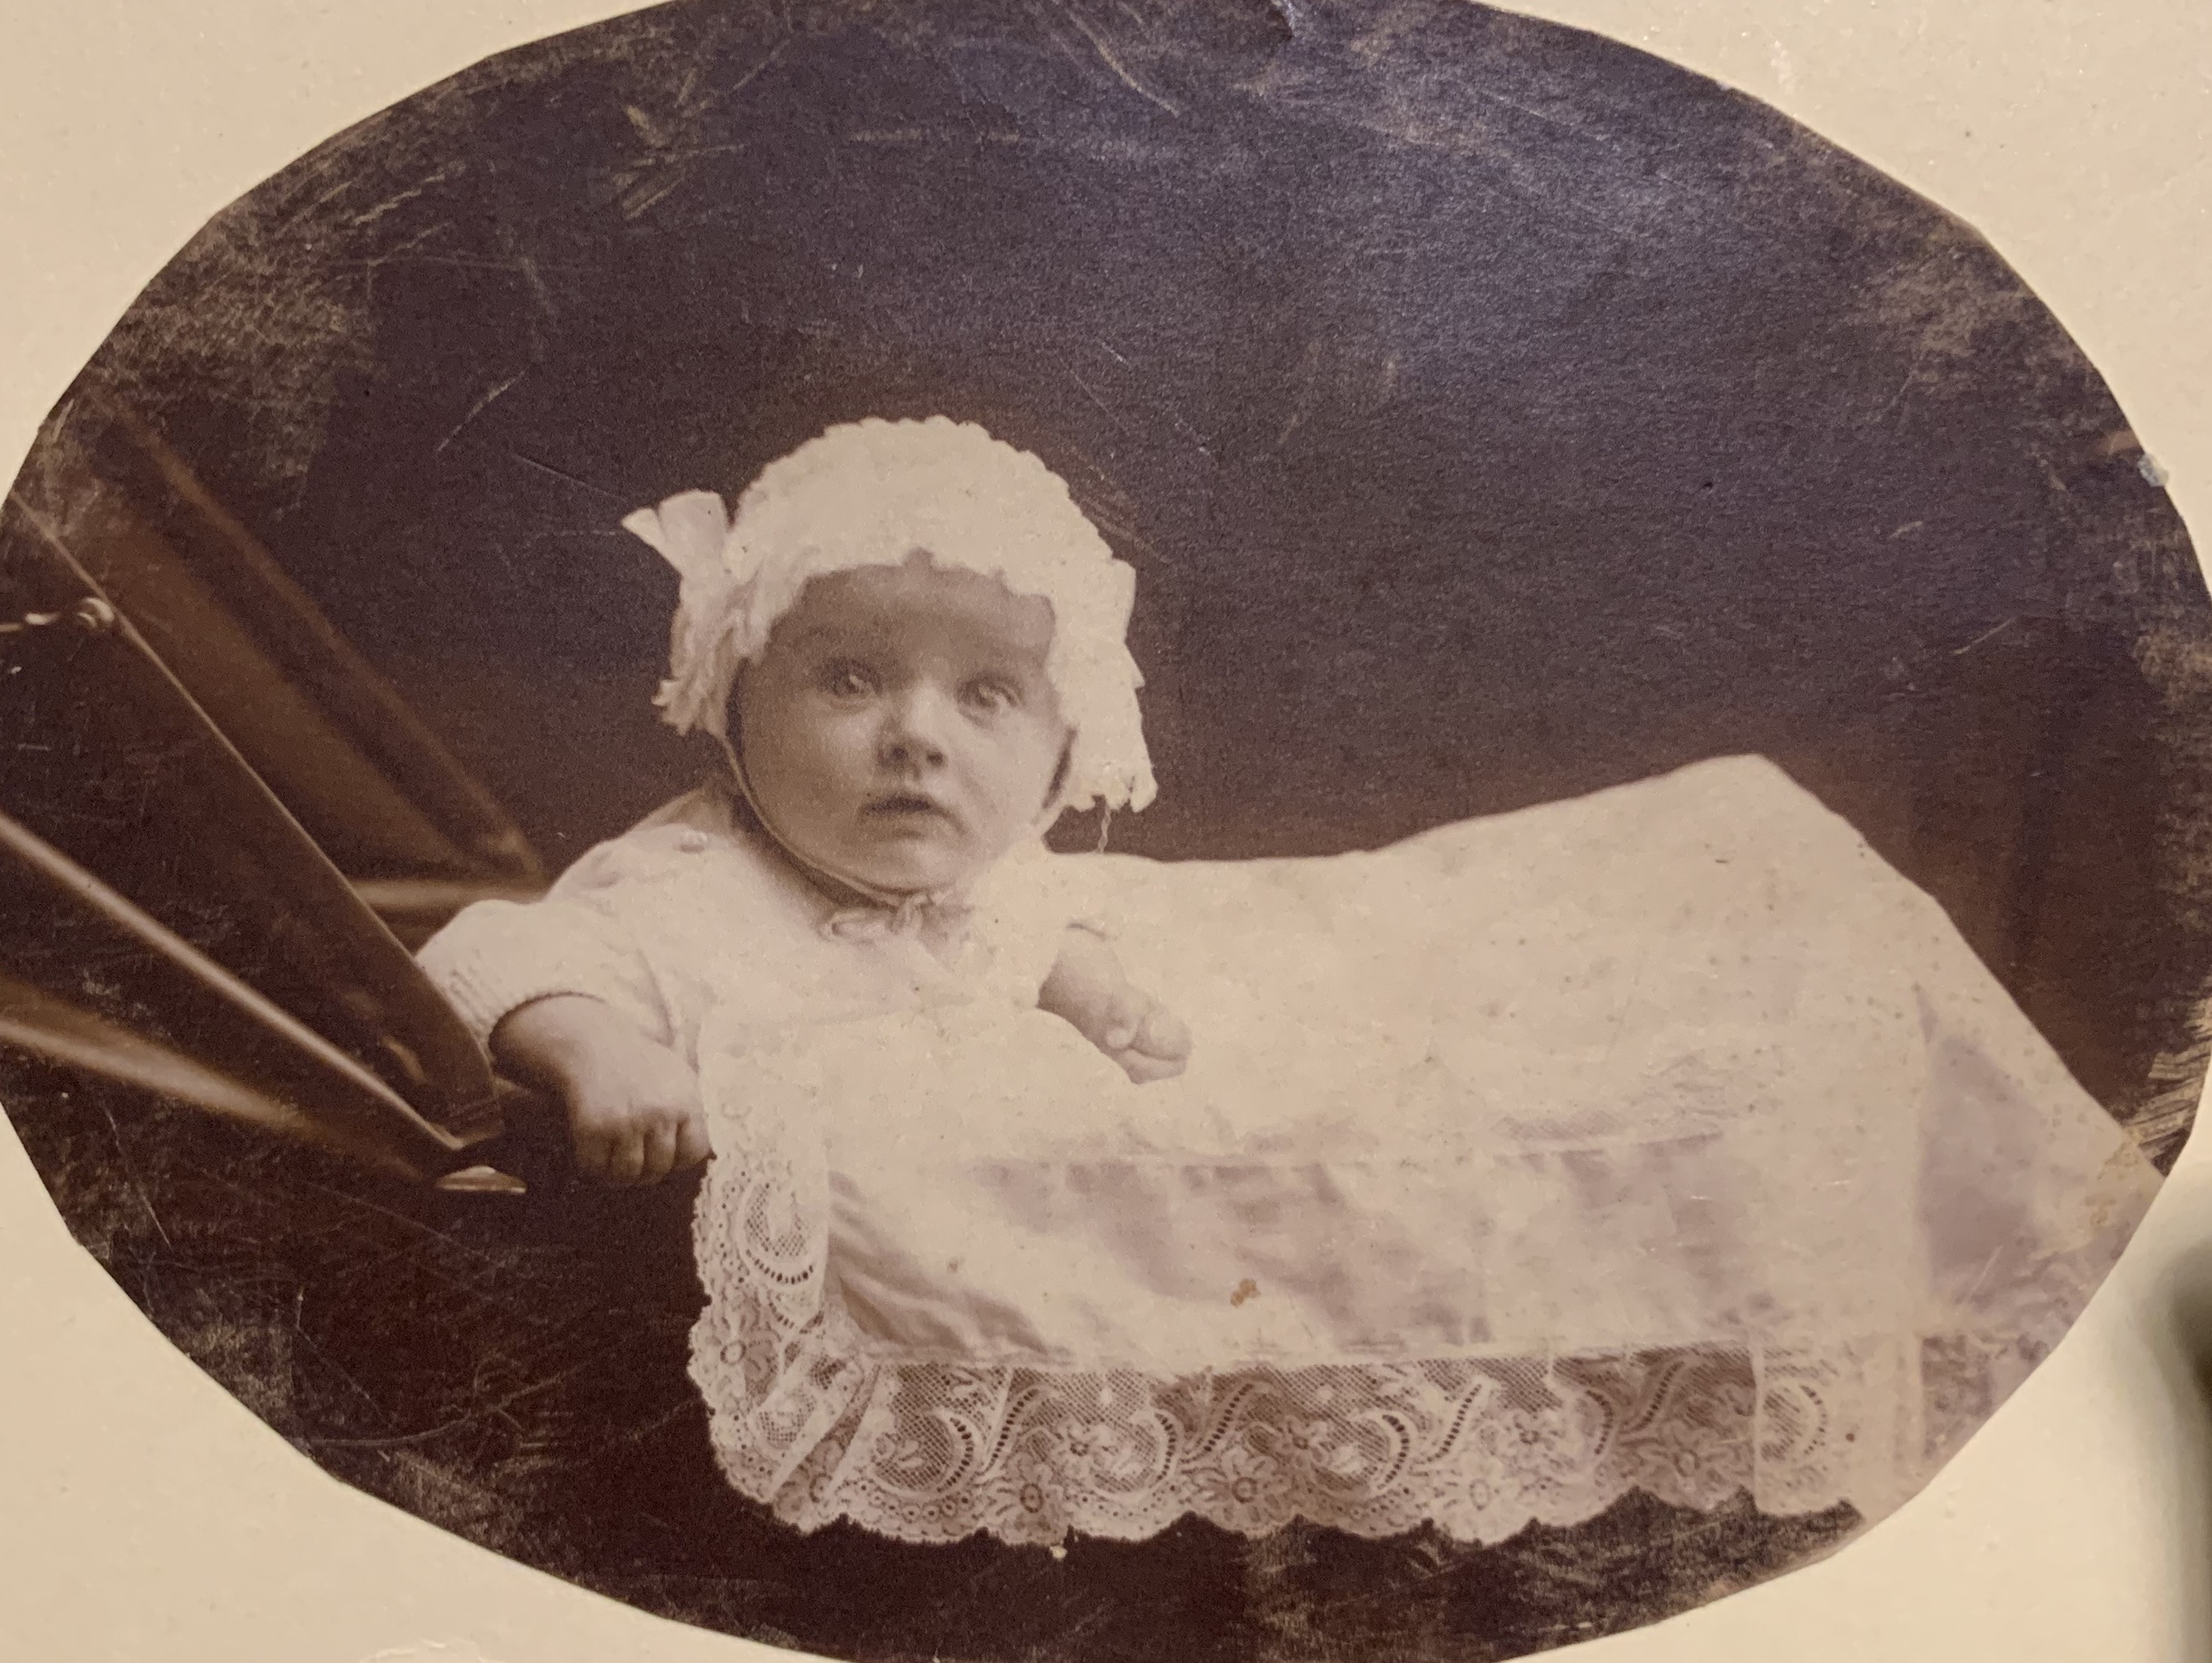
\includegraphics[width=1\textwidth]{boek_Tine_Blom.docx.tmp/word/media/image3.jpg}

Vanaf 6 ging je lopend naar school. Het hoofd van de school woonde tegenover ons. Kwam Bert een keer thuis met een waterpistool; ze wilden op de meester schieten maar durfden het niet. Toen vroegen ze aan mij om dat te doen! Je weet niet hoe hard we daarna wegliepen! Toen kreeg m’n moeder de buurman aan de deur. Ze hadden een dochter en die had een eigen speelkamer.

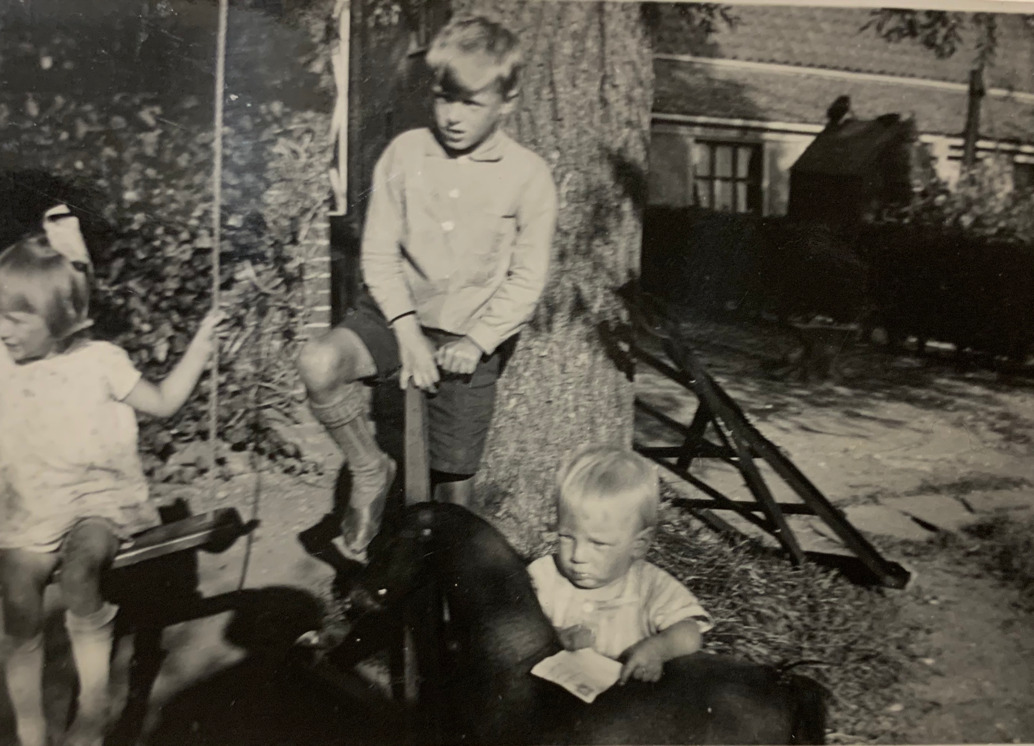
\includegraphics[width=1\textwidth]{boek_Tine_Blom.docx.tmp/word/media/image4.jpg}

Ik speelde veel met Kees vroeger. We konden goed samen spelen. Kees had ook wel zijn vriendjes en ik mijn vriendinnen. We hadden ringen in de bijkeuken hangen en een schommel buiten.

\textit{De schommel in de tuin}

Mijn moeder had toen al een wasmachine; die stond in de smederij. Want daar stond een slijpmachine en daar werd de wasmachine ook aangesloten. Er was een kooktoestel in de bijkeuken en in de winter zaten we daar. In het voorjaar gingen de mooie stoelen weer naar de voorkamer en aten we daar.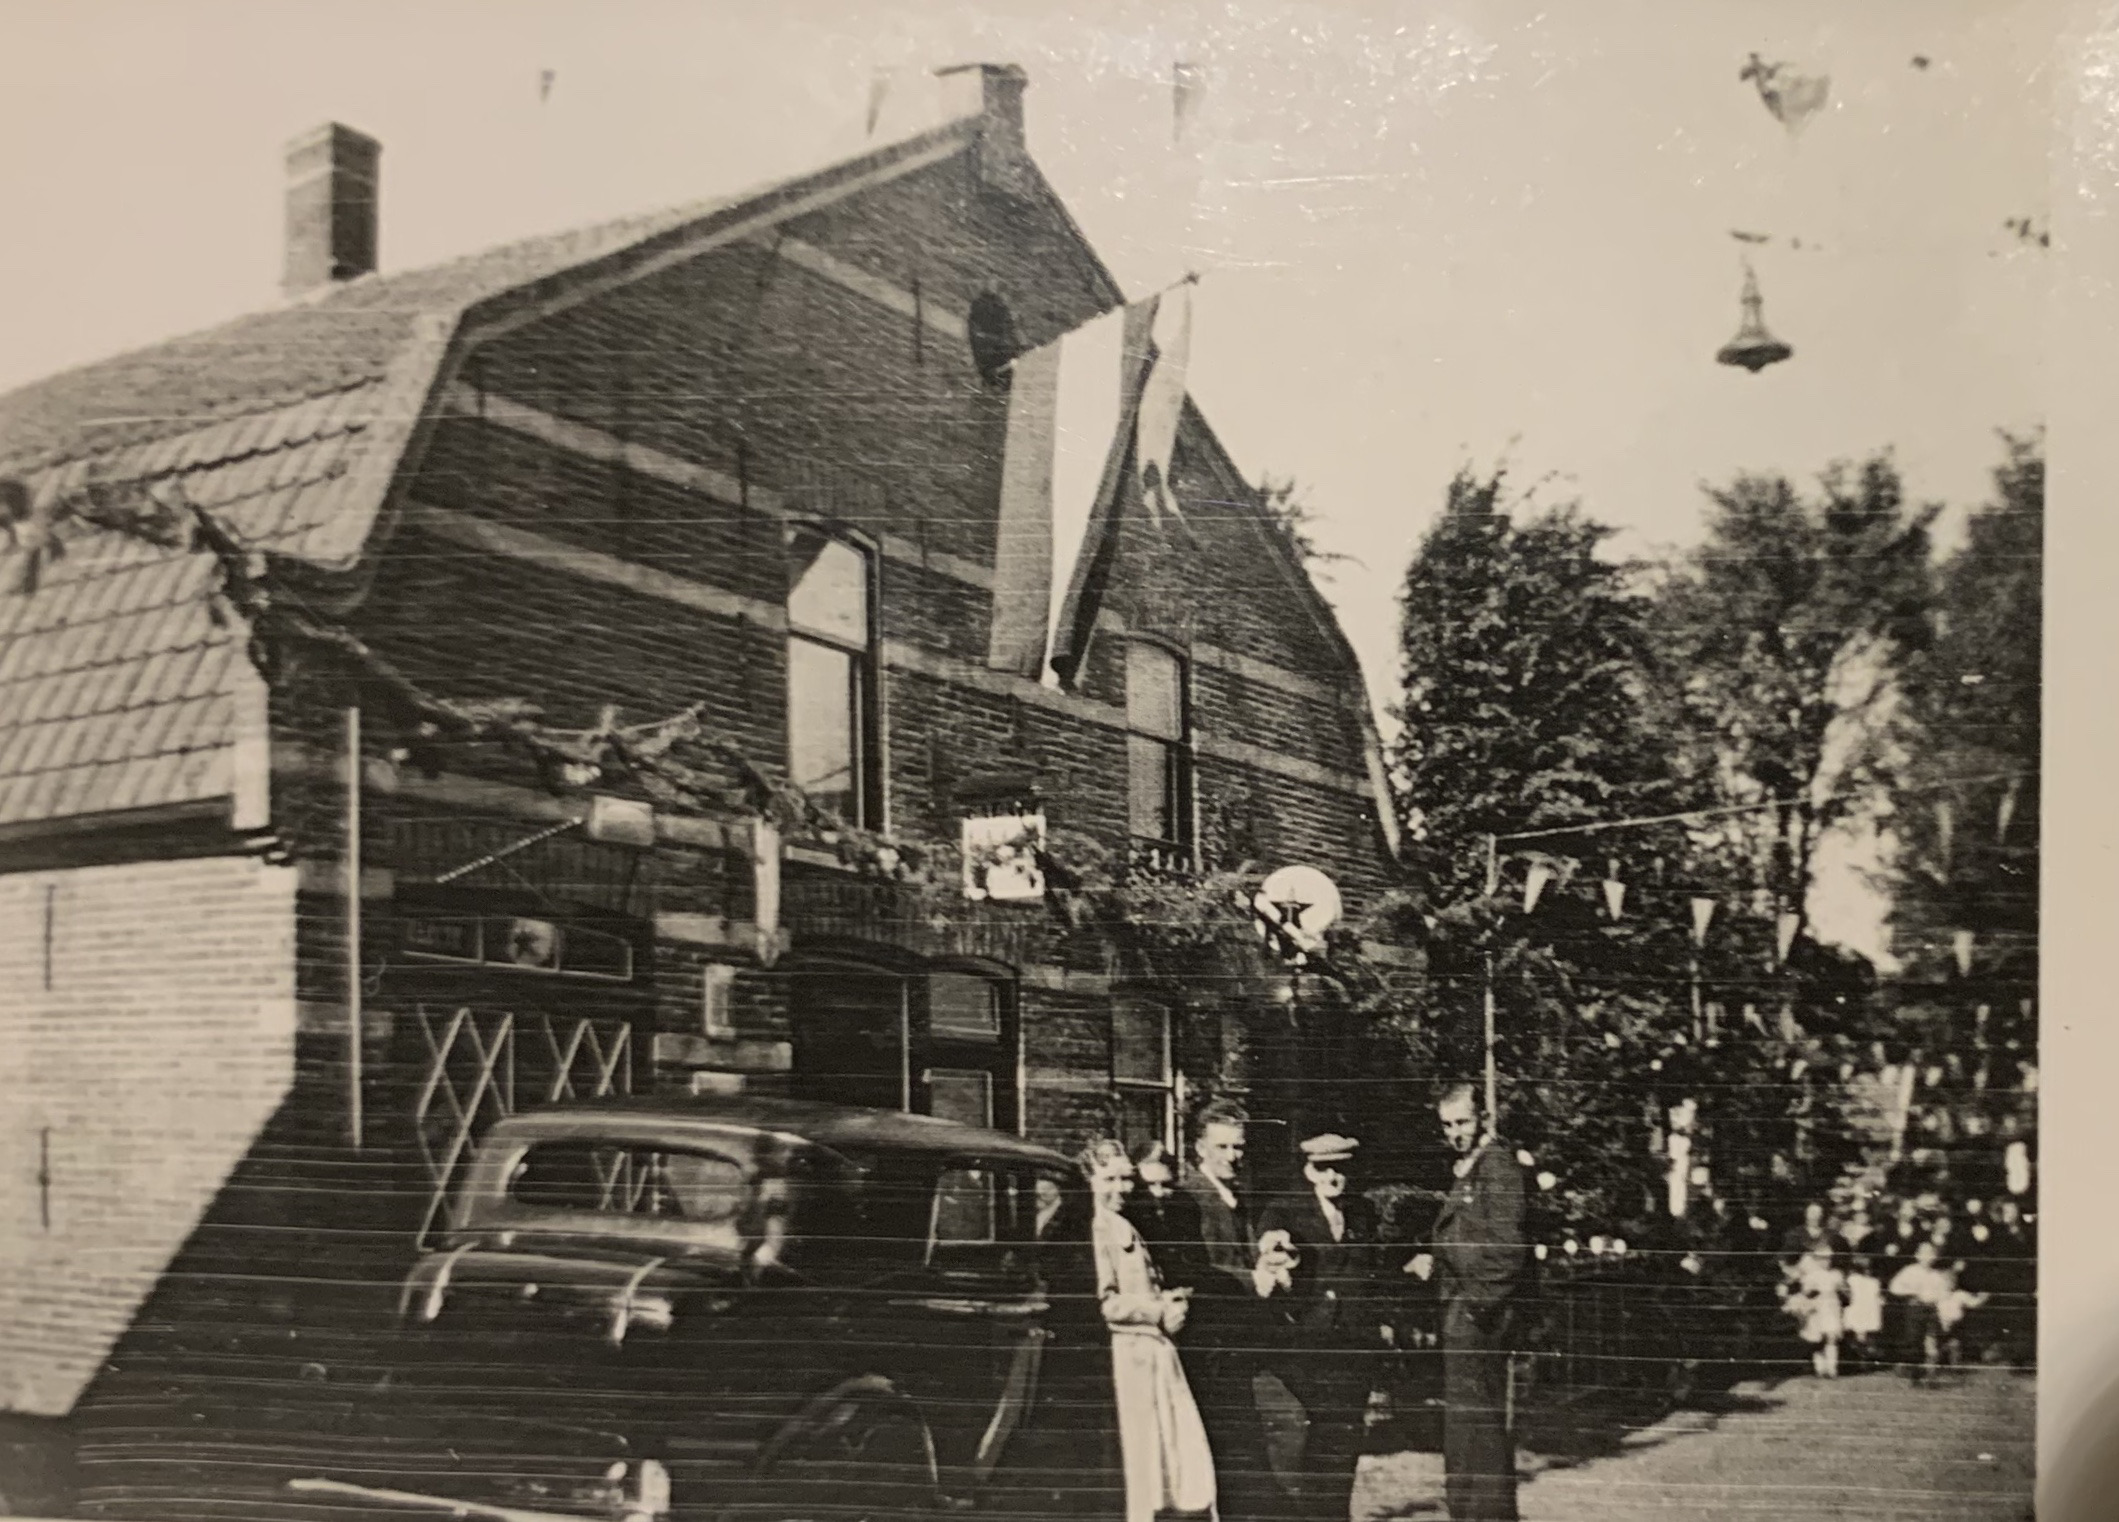
\includegraphics[width=1\textwidth]{boek_Tine_Blom.docx.tmp/word/media/image5.jpg}

\textit{Het huis in Oudkarspel}

In de bijkeuken was ook een bedstee en daar sliepen de jongens.

Als klein kind sliep ik in de bedstee bij m’n ouders. Toen ik groter werd kreeg ik de kamer op zolder.

Eerst hadden we een WC buiten, achter de garage, boven het water. Maar toen ik jong was kregen we al
een WC binnen. In Langedijk, als je daar ging varen, voer je de hele tijd onder de buiten-Wc's van de mensen door.

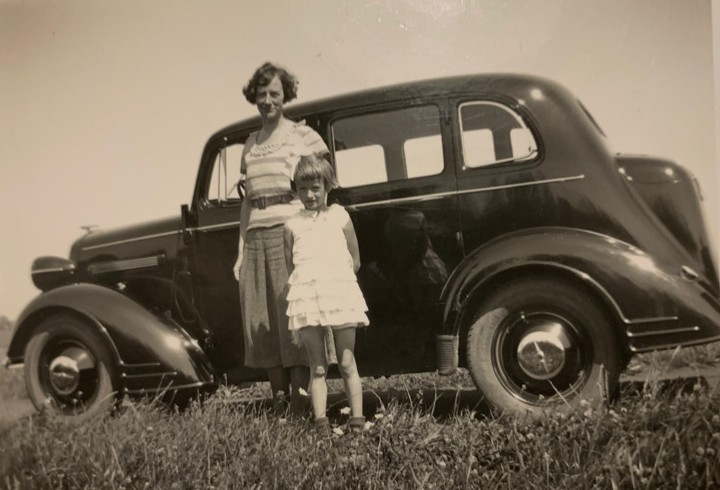
\includegraphics[width=1\textwidth]{boek_Tine_Blom.docx.tmp/word/media/image6.jpg}

Iedere zondag gingen we naar het strand bij Camperduin. Dat was gezond vond m’n moeder.
We hadden een grote tent mee waar je je kon verkleden. We gingen met de auto daarheen. Voor m’n vader was dat niet altijd zo leuk want hij was dan moe van het bedrijf en het was een heel gesjouw met al die spullen.

\textit{met de auto naar het strand}

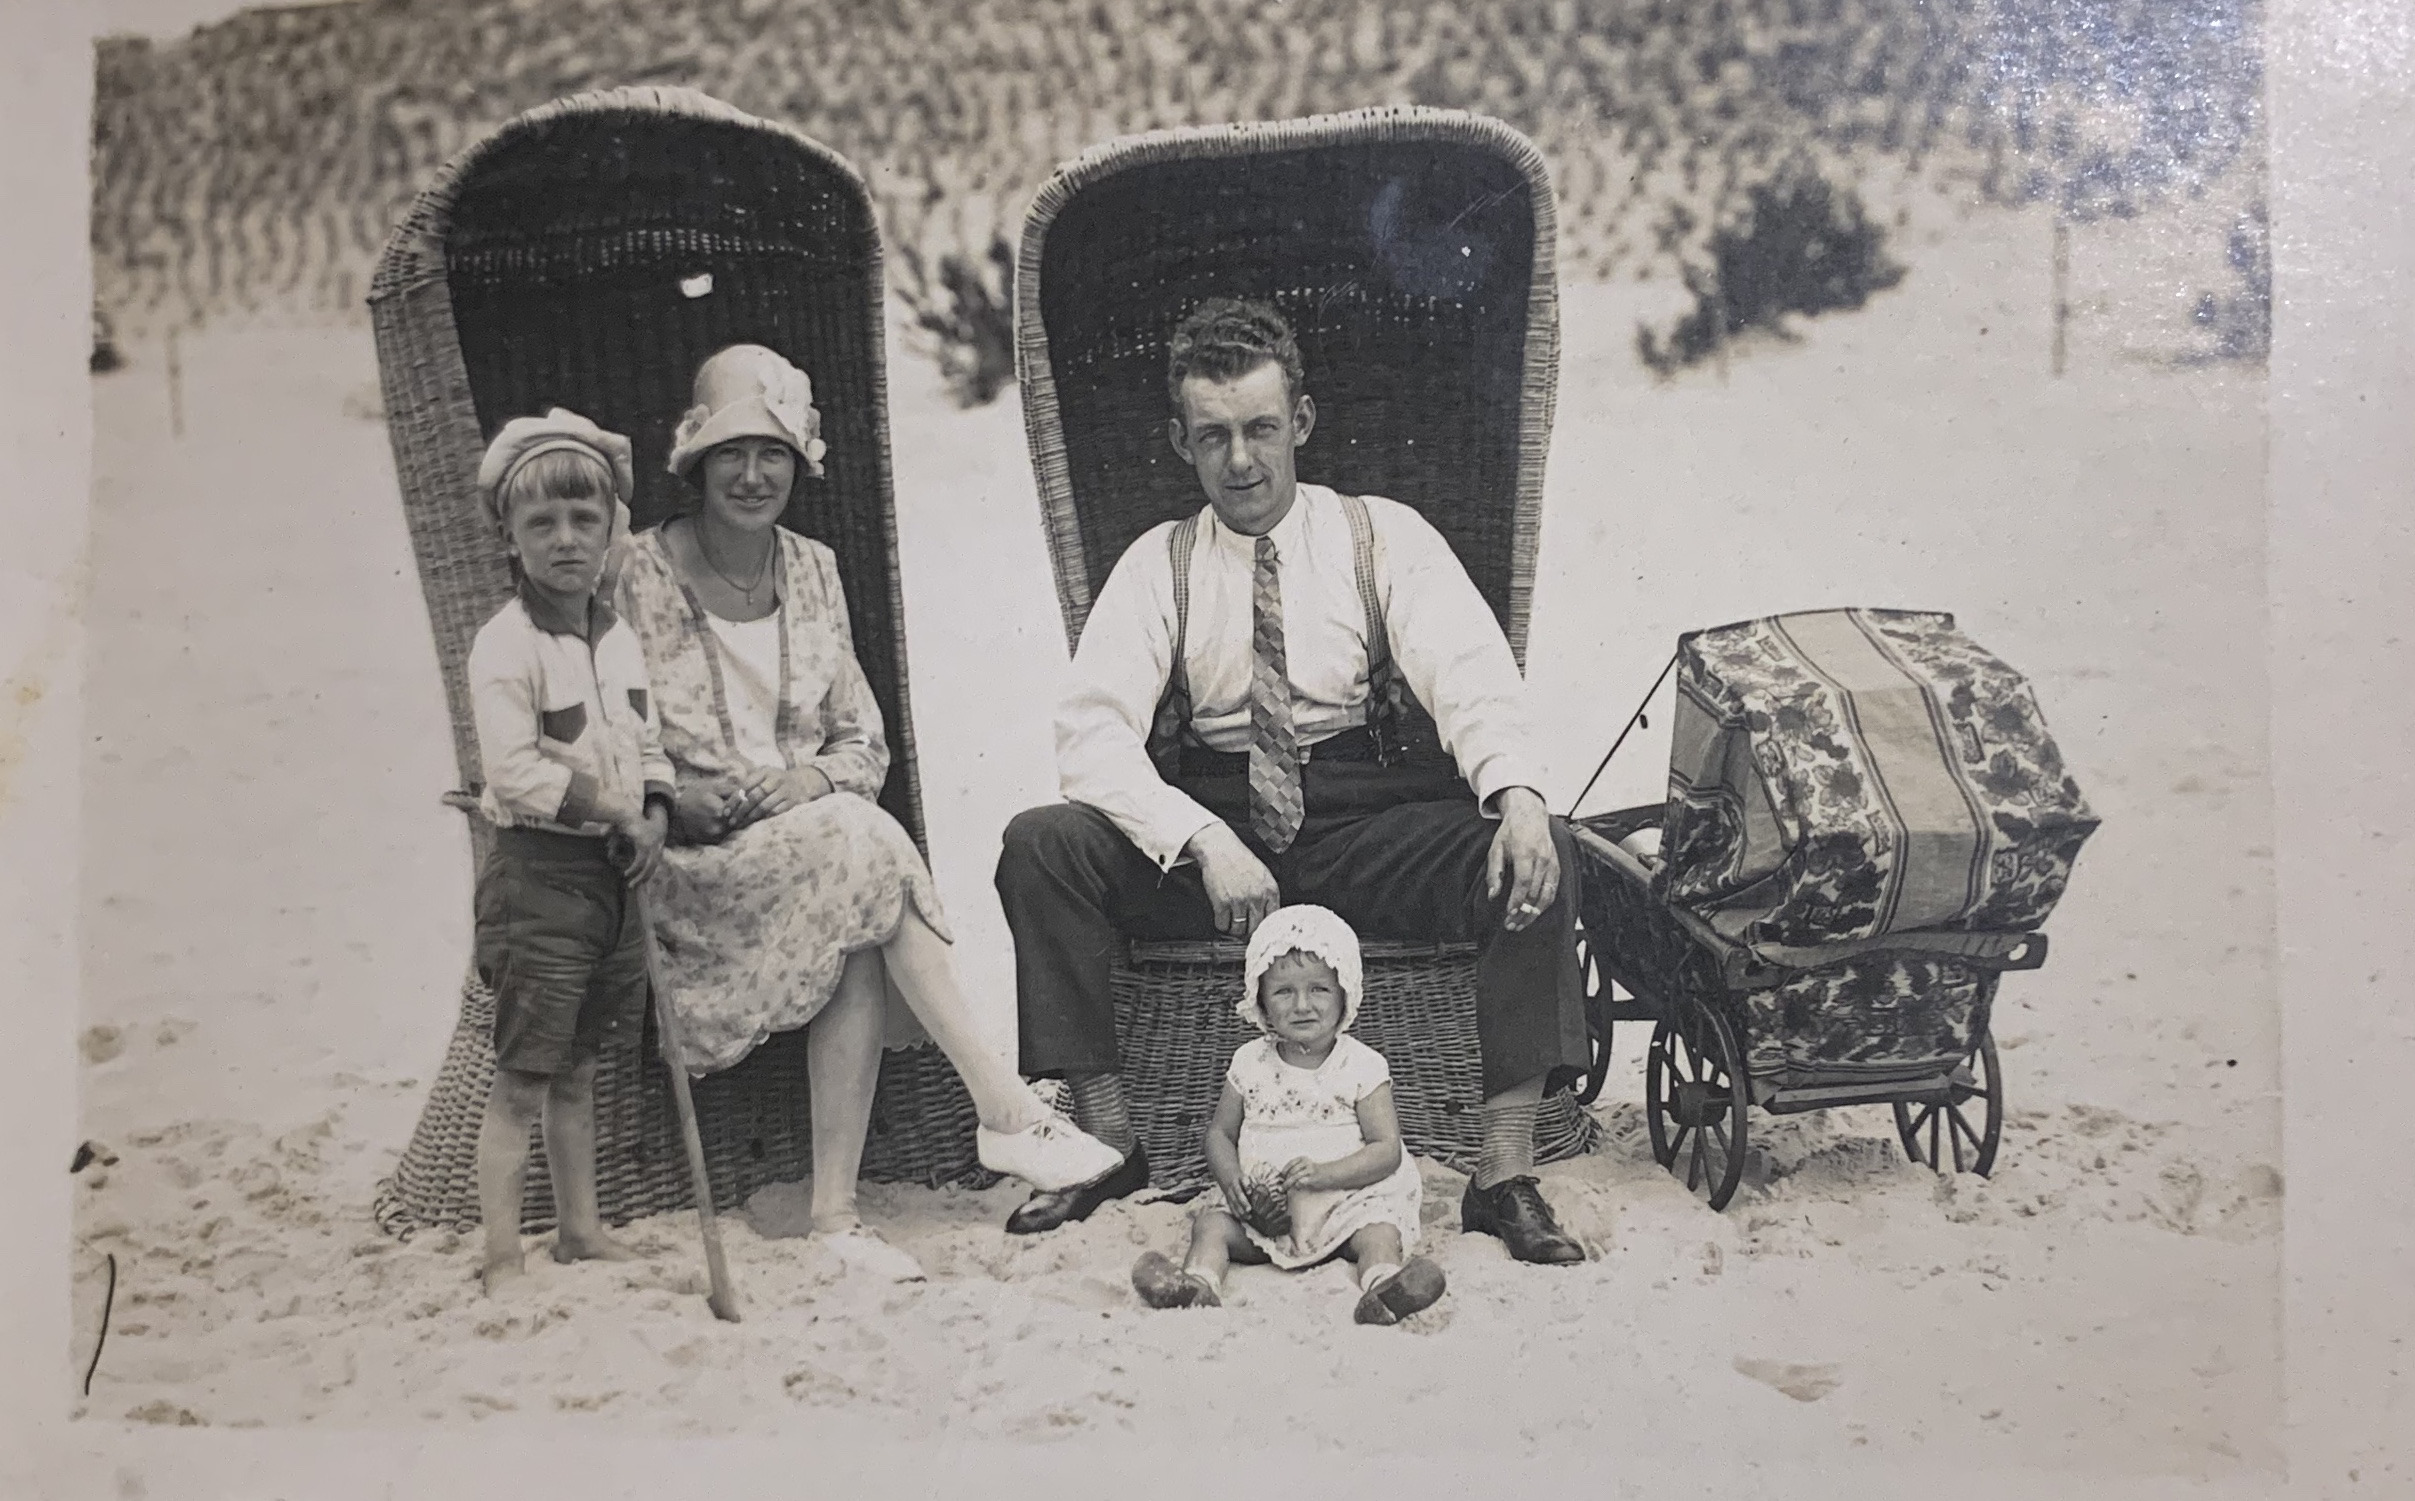
\includegraphics[width=1\textwidth]{boek_Tine_Blom.docx.tmp/word/media/image7.jpg}

\textit{Het gezin aan het strand}

Bert was als kind altijd een beetje minnetjes. Veel ziek. Hij was heel veel op de boerderij van mijn grootouders in Schoorldam, dan was hij gelijk buiten. 

Mijn vader heeft toen een bokkenwagen gemaakt en opa hielp om de bok voor de kar te zetten.

We gingen ook vaak nog even aan in Schoorldam, bijna elke week.

En \'{e}\'{e}n keer zijn we met opa Vlam vanaf Schoorldam met een mooi rijtuig en een paard ervoor naar het strand geweest. Een rijtuig met van die kussens aan weerskanten. Op Camperduin kende hij mensen waar hij het paard kon stallen. Dat was een geweldige belevenis.

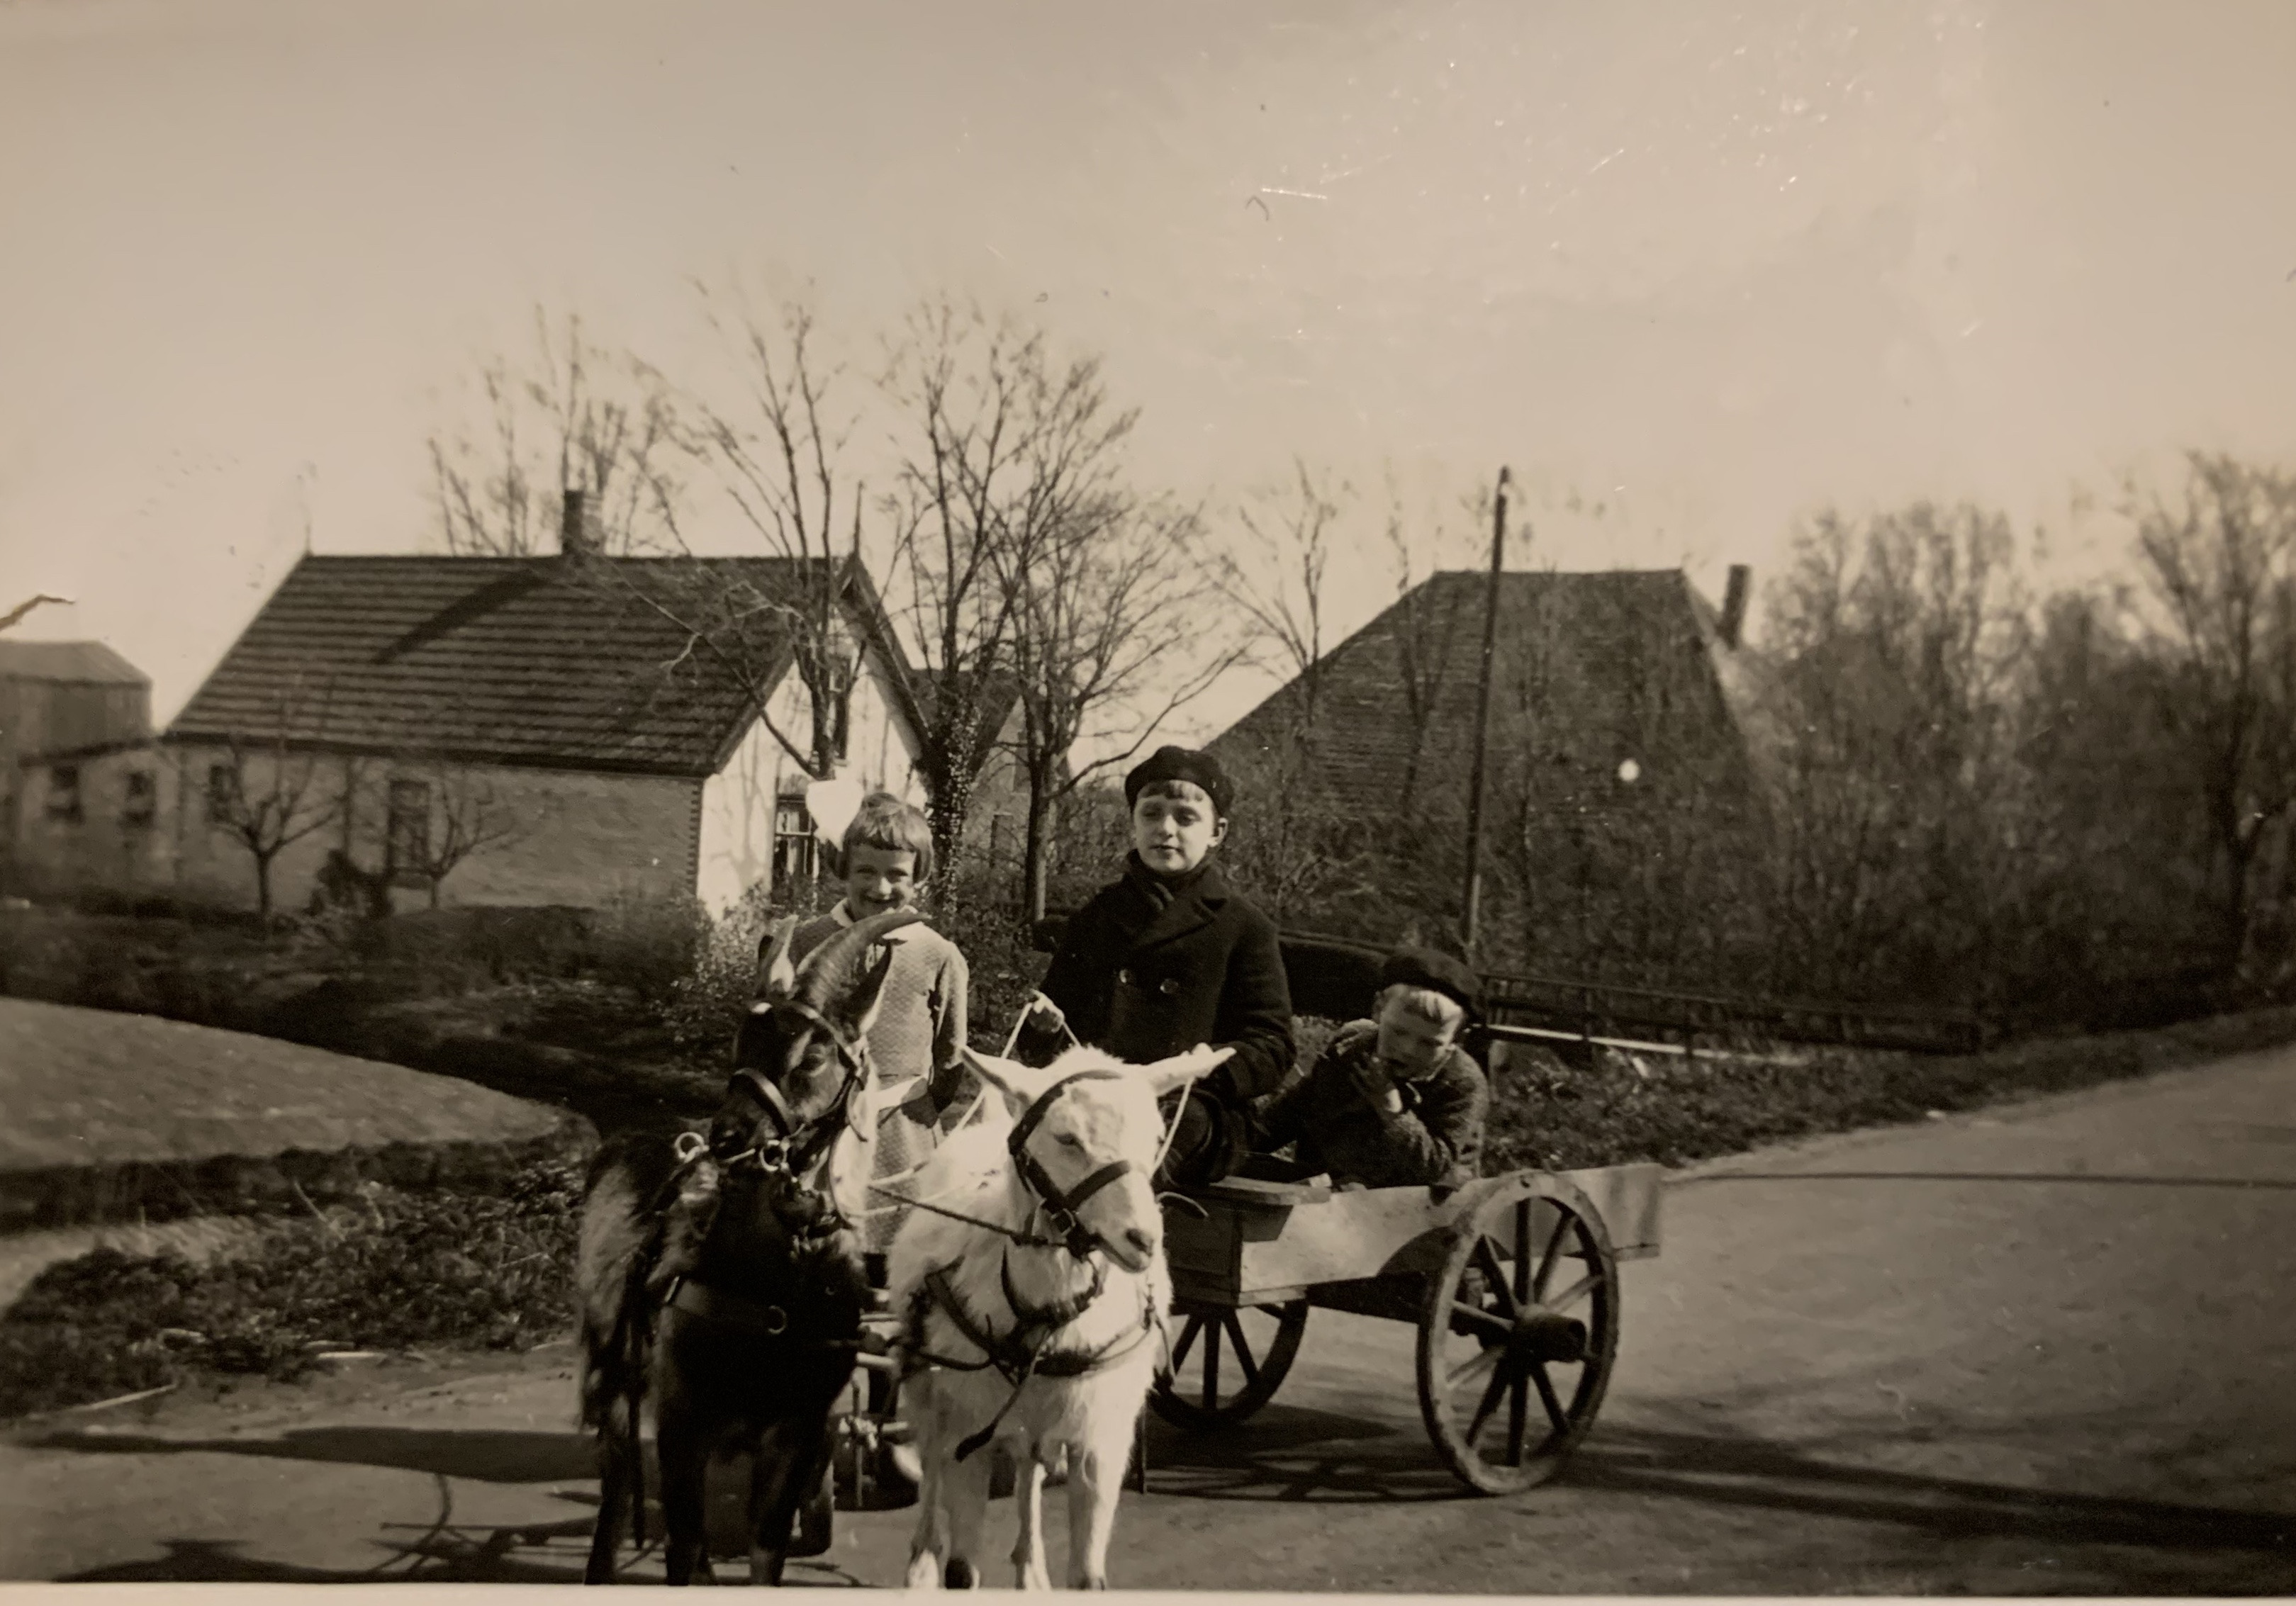
\includegraphics[width=1\textwidth]{boek_Tine_Blom.docx.tmp/word/media/image8.jpg}

Mijn vader had een heel bedrijf; een smederij, een winkel en een grote garage. Daar stond de dorsmachine die door het hele dorp werd gehuurd. Als hij gebruikt werd stond hij op een veldje verderop en dan kwamen alle landbouwers met hun graan; dat kwam dan in zakken. 

\textit{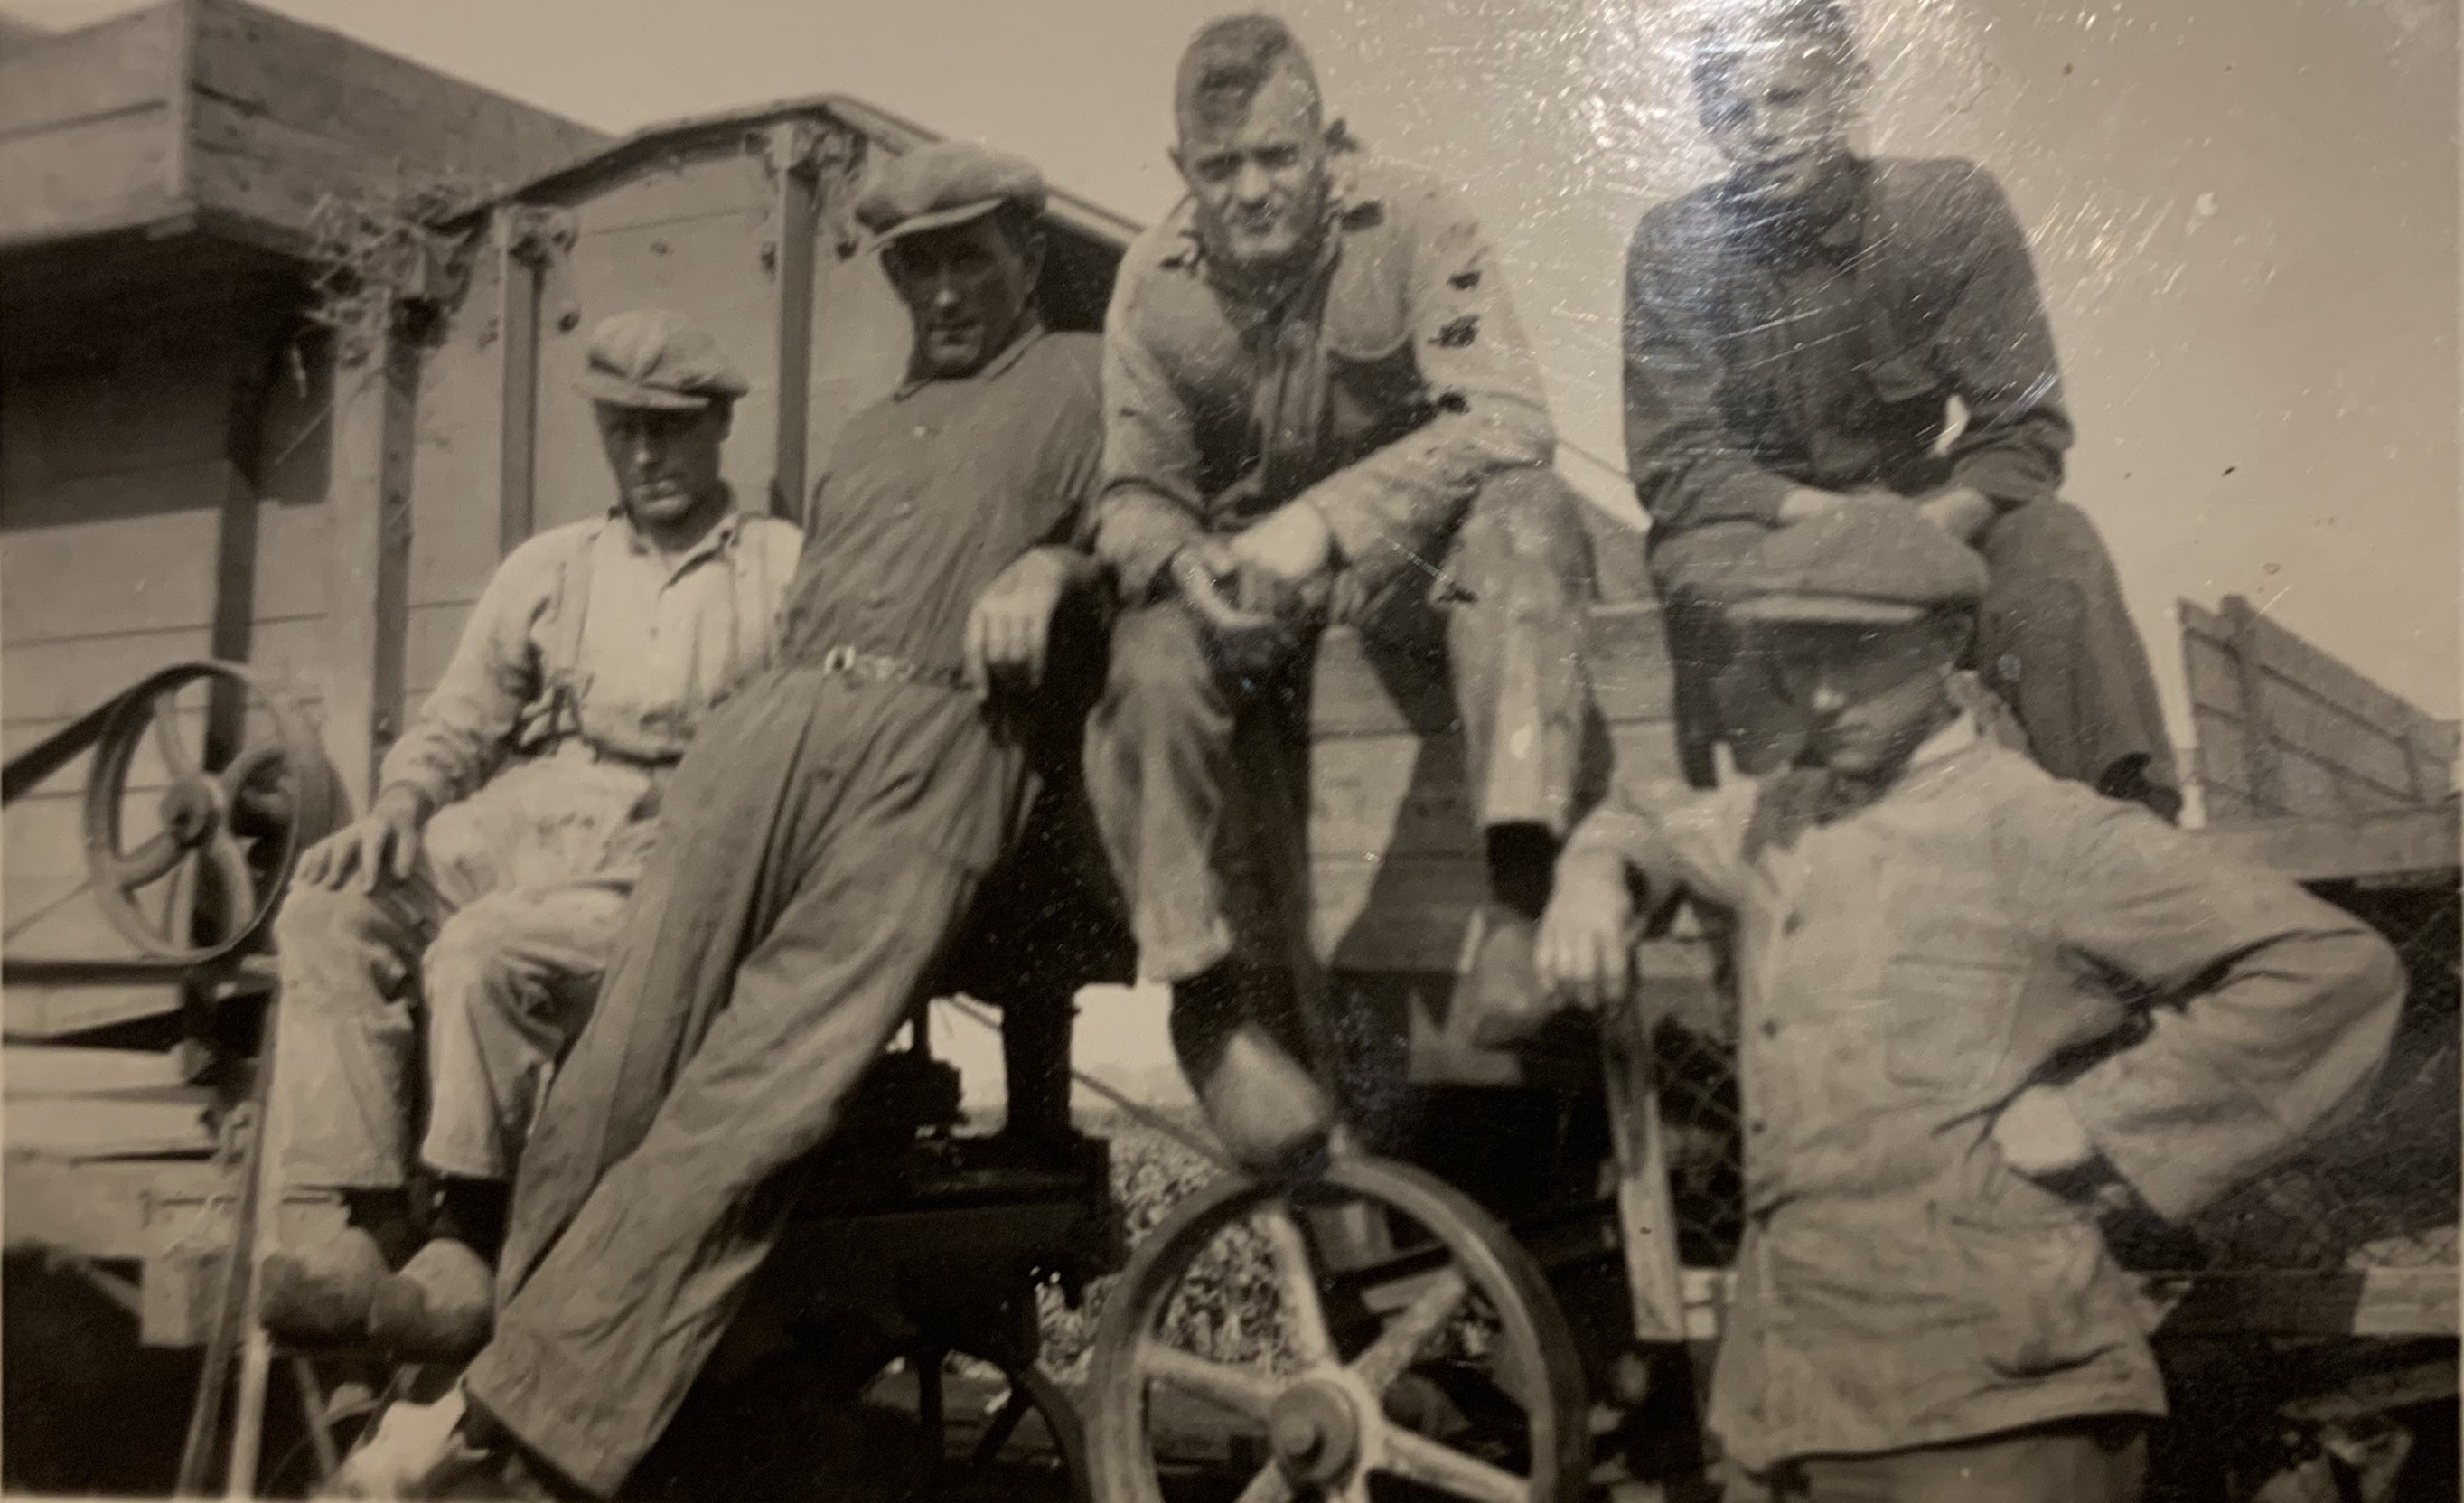
\includegraphics[width=1\textwidth]{boek_Tine_Blom.docx.tmp/word/media/image9.jpg}}

\textit{De dorsmachine}

Iedereen kwam met bootjes naar dat veld. Het land van de duizend eilanden heette het. Iedereen had een veldje tussen het hoge water in. De bootjes werden vooruitbewogen met een kloet. Kees vond het ook prachtig om daarbij te zijn, het dorsen.

In de garage stonden ook een aantal auto’s; die werden verhuurd.

Het huis in Oudkarpsel is later gesloopt, het staat er nu niet meer. Mijn opa en oma, de ouders van mijn vader, woonden vlakbij. Zij woonden in een klein huisje achter ons huis. Een huisje met twee bedsteden.

Wij roeiden ook veel. Toen ik een keer bij de dokter was zei hij dat ik zulke sterke schouders had. Dat kwam van het roeien denk ik.

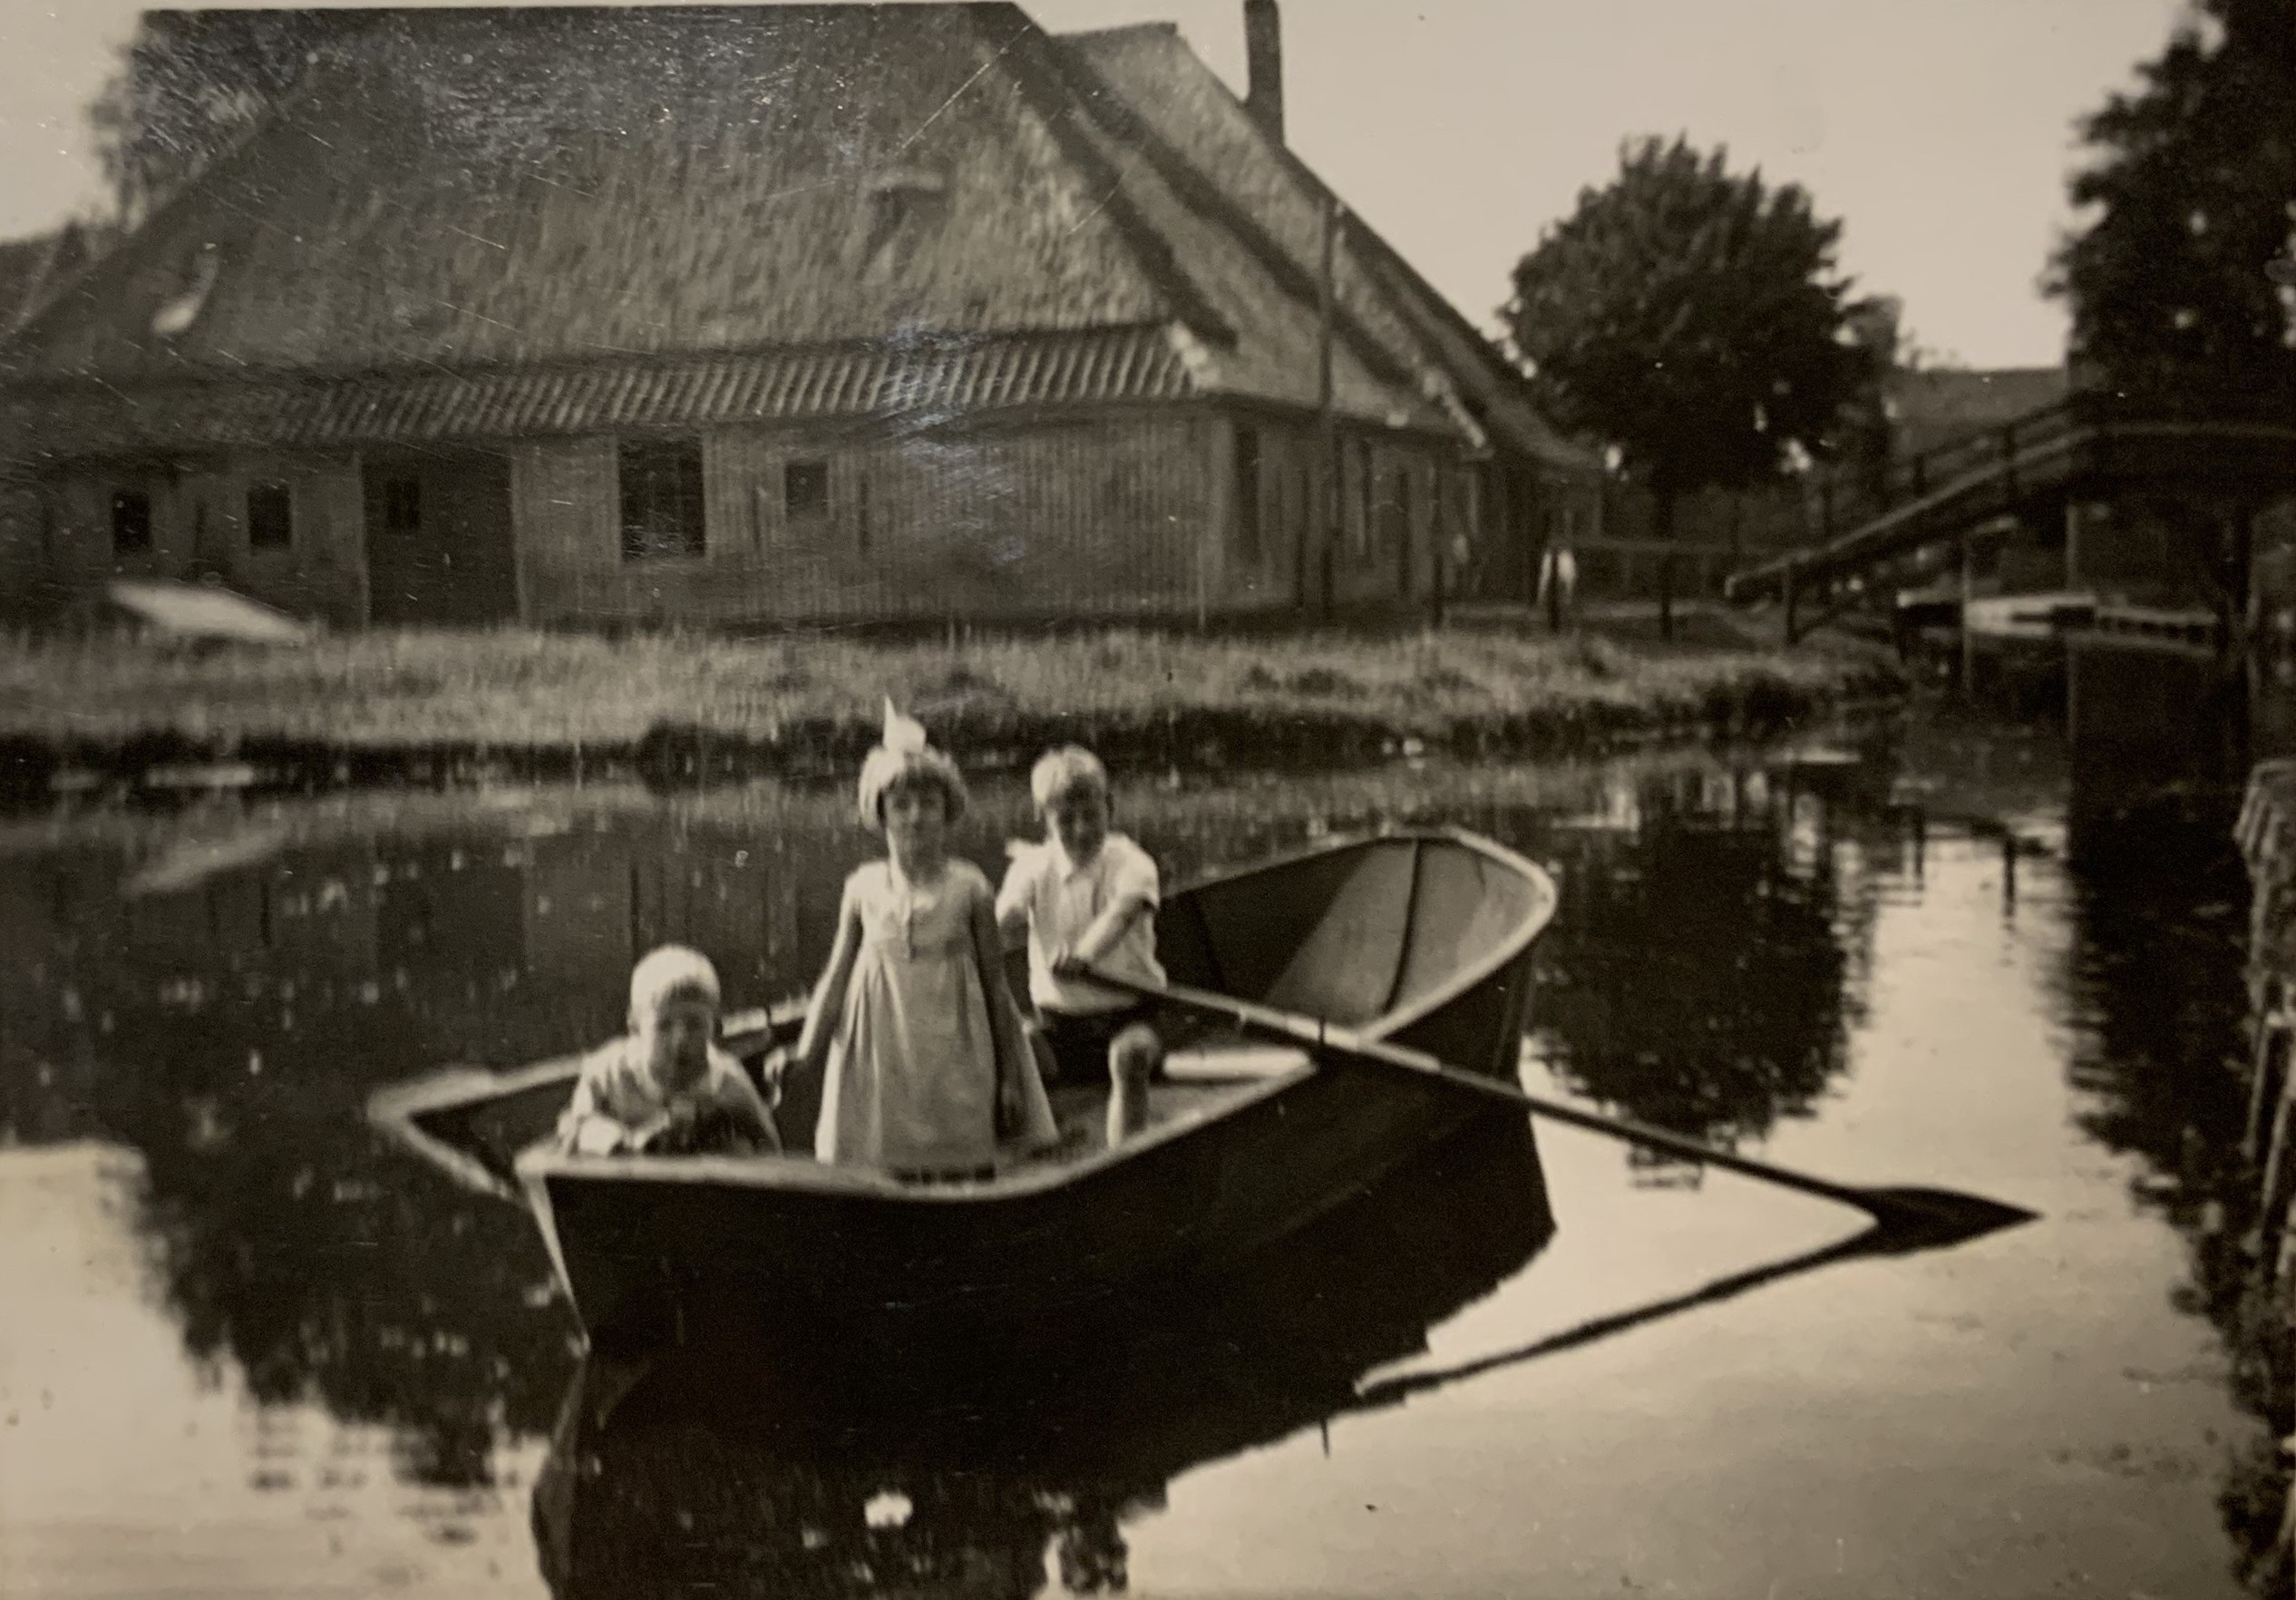
\includegraphics[width=1\textwidth]{boek_Tine_Blom.docx.tmp/word/media/image10.jpg}

\textit{Bert aan het roeien met Tine en Kees}

\chapter{\label{ref-003}Ouders en Voorouders}

Mijn ouders zijn tegelijkertijd getrouwd met haar broer, Piet Vlam en zijn vrouw. 

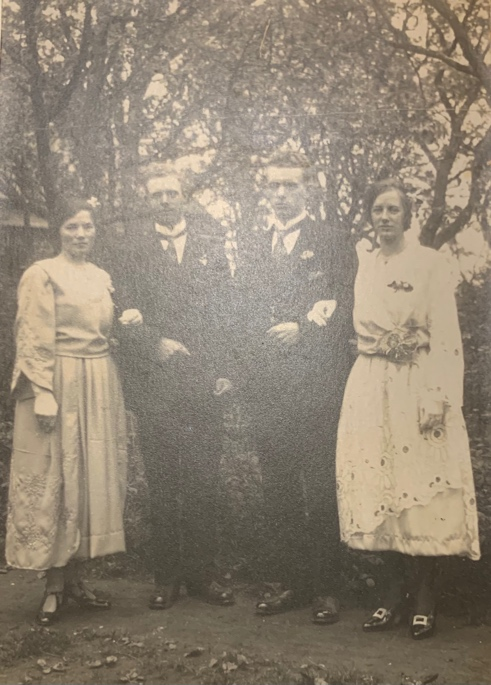
\includegraphics[width=1\textwidth]{boek_Tine_Blom.docx.tmp/word/media/image11.jpeg}
Met die broer had ze verder niet veel contact overigens. Ik vond het ook geen leuke man.
Volgens mijn moeder was hij als kind wel leuk maar is hij zo geworden door zijn vrouw. Dat was een beetje een haaiebaai.

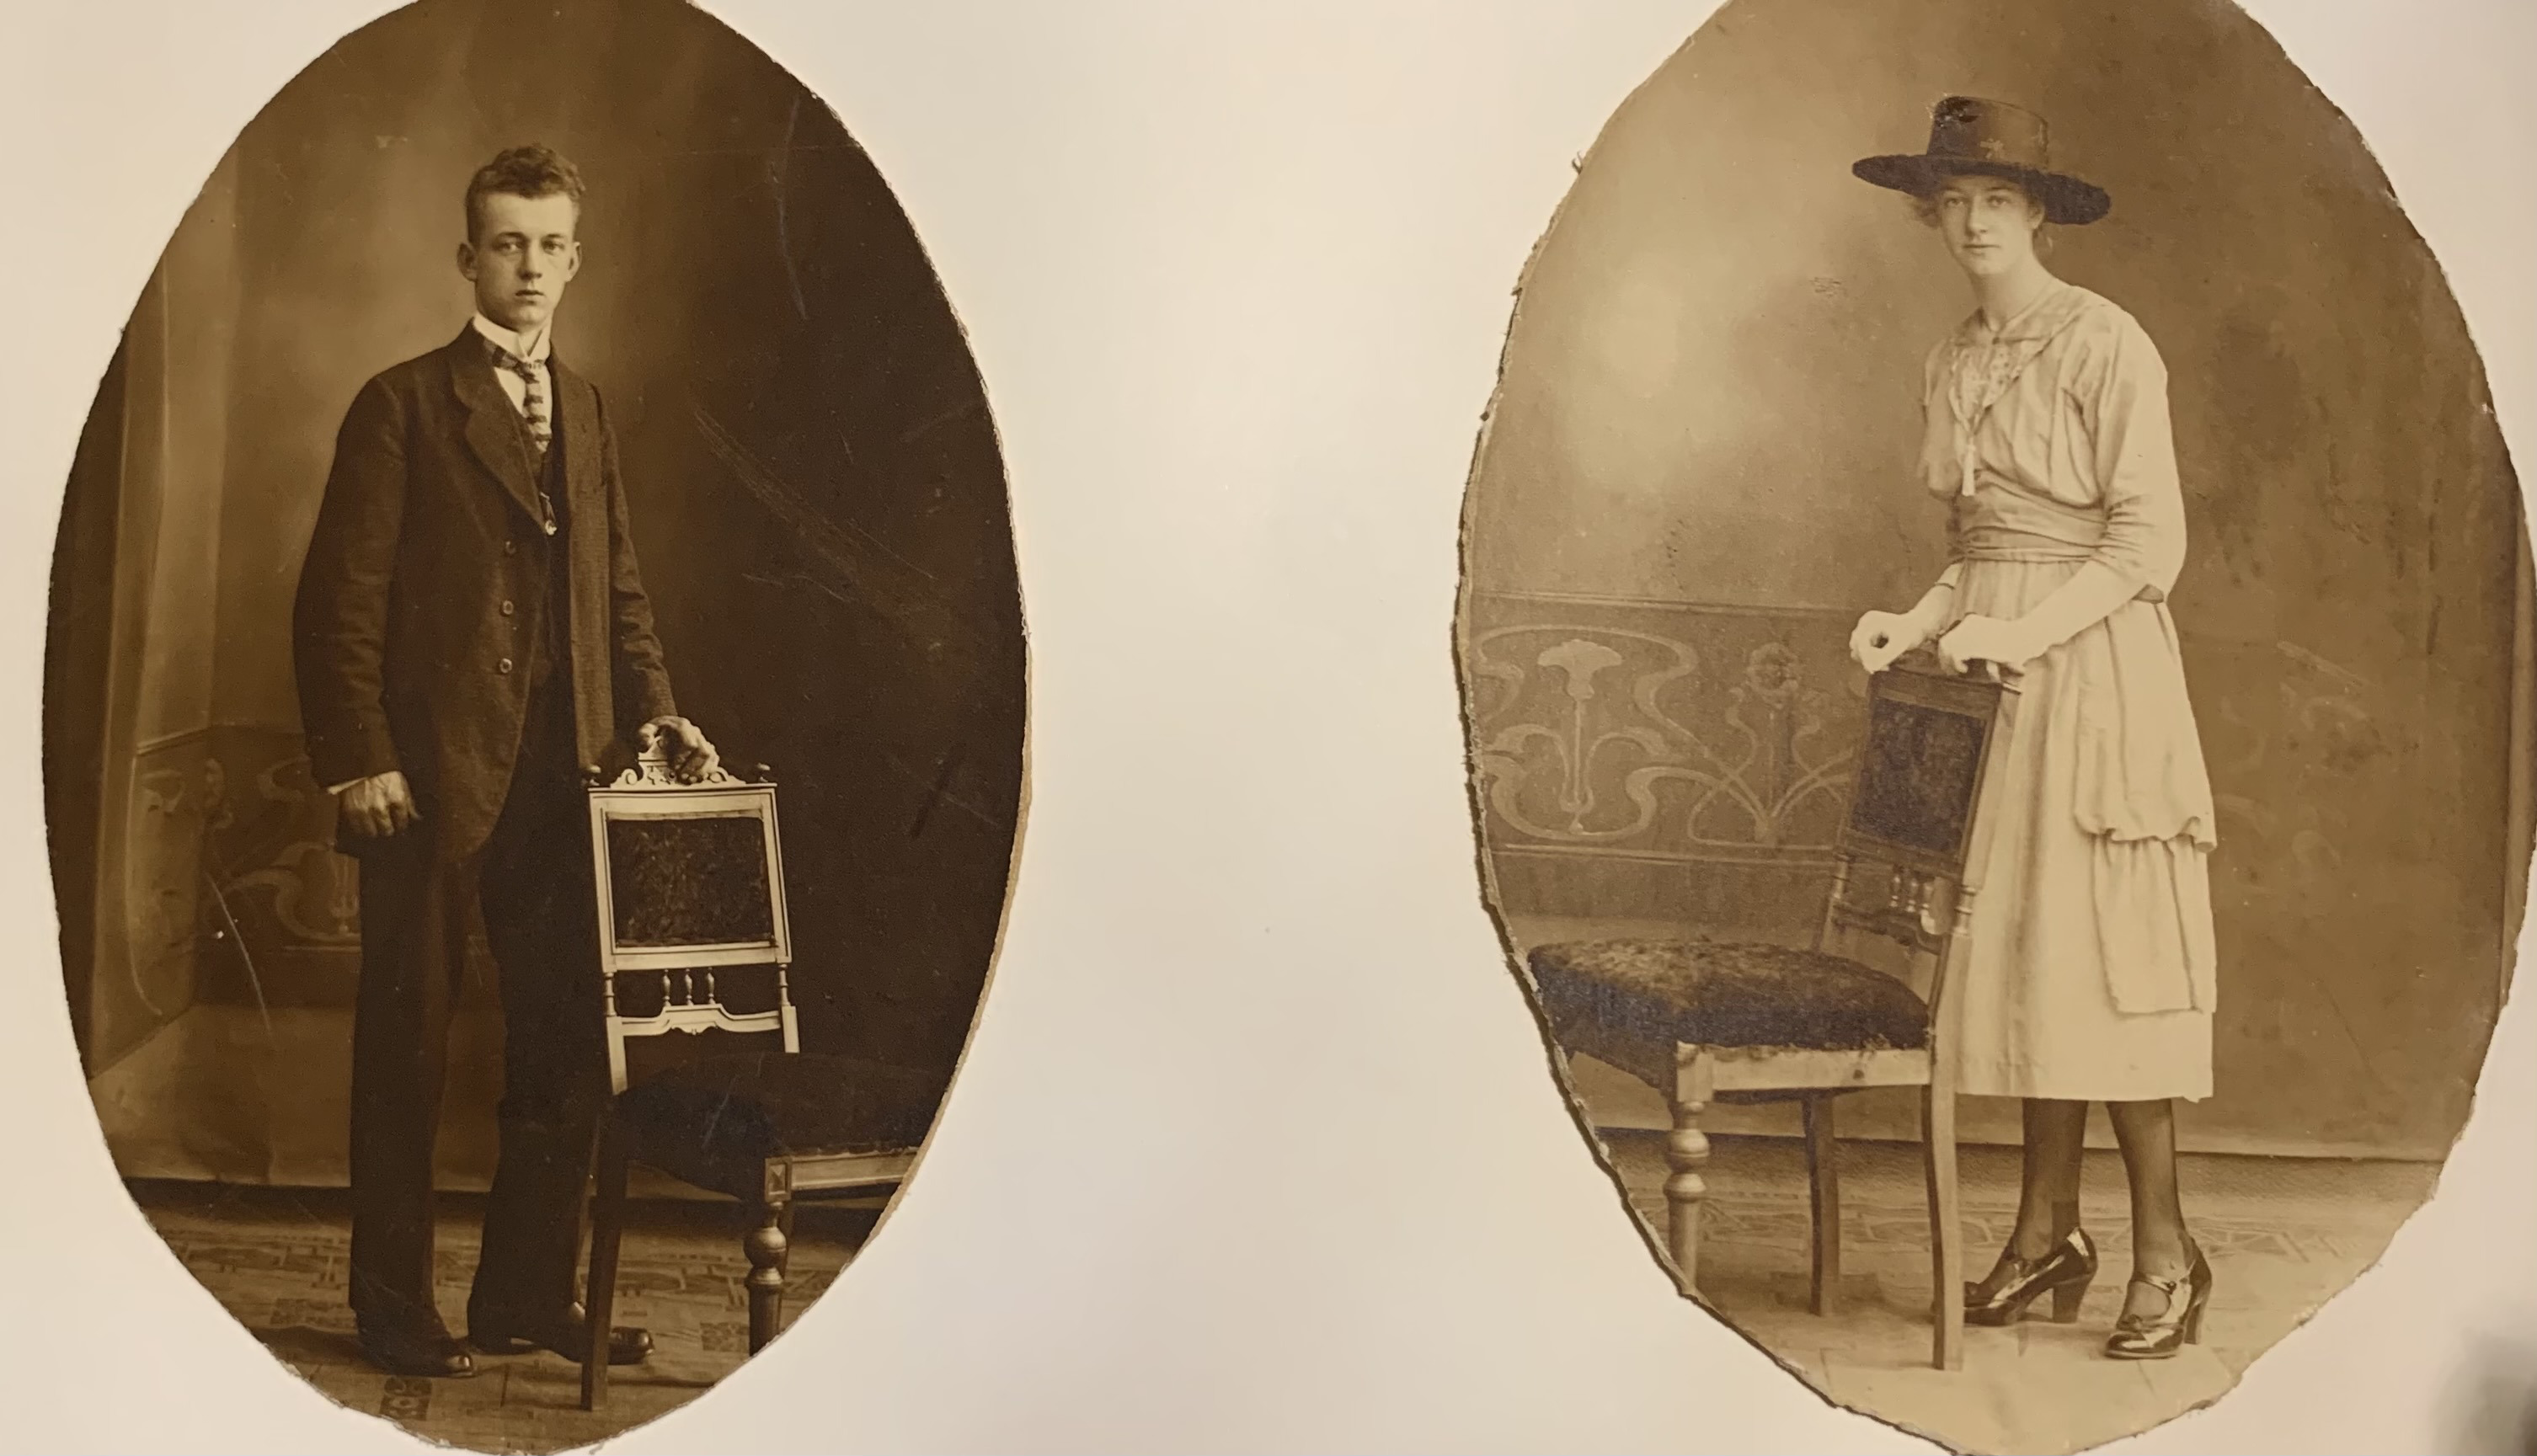
\includegraphics[width=1\textwidth]{boek_Tine_Blom.docx.tmp/word/media/image12.jpg}

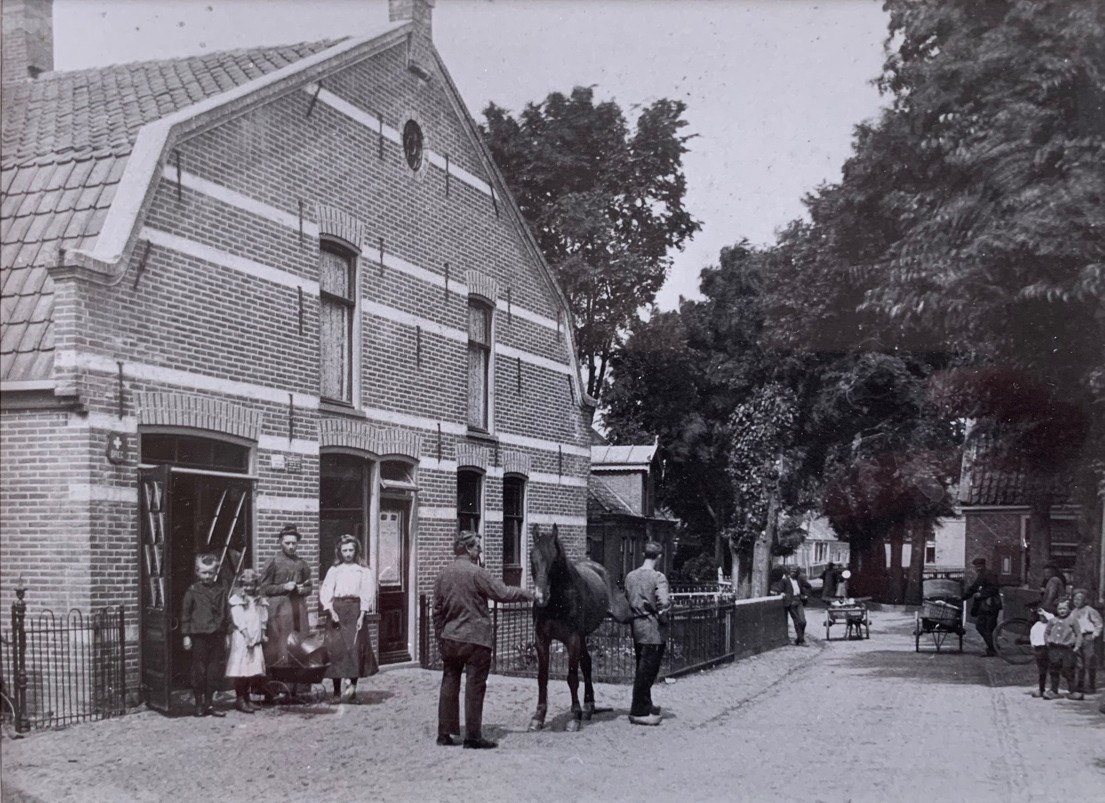
\includegraphics[width=1\textwidth]{boek_Tine_Blom.docx.tmp/word/media/image13.jpeg}

Mijn vader kwam uit Oudkarspel. Zijn ouders hadden daar de smederij in het huis waarin ik ben geboren. 

\textit{De smederij; links mijn vader als jongetje, met zijn moeder en zussen. De smid is mijn opa.}

Zijn voorouders kwamen allemaal uit Noord-Holland; o.a. uit Enkhuizen. 

Hij had twee zussen. Die heetten Trien en Rentsje.

Hij was ondernemend en goed opgeleid, eerst tot smid, en later heeft hij in Antwerpen nog een opleiding m.b.t. auto’s gevolgd.

In hun verkeringstijd haalde hij mijn moeder op met de motor. Hij was de bink van de streek. Er was toen zo weinig verkeer dat ze hem al van verre hoorde aankomen.

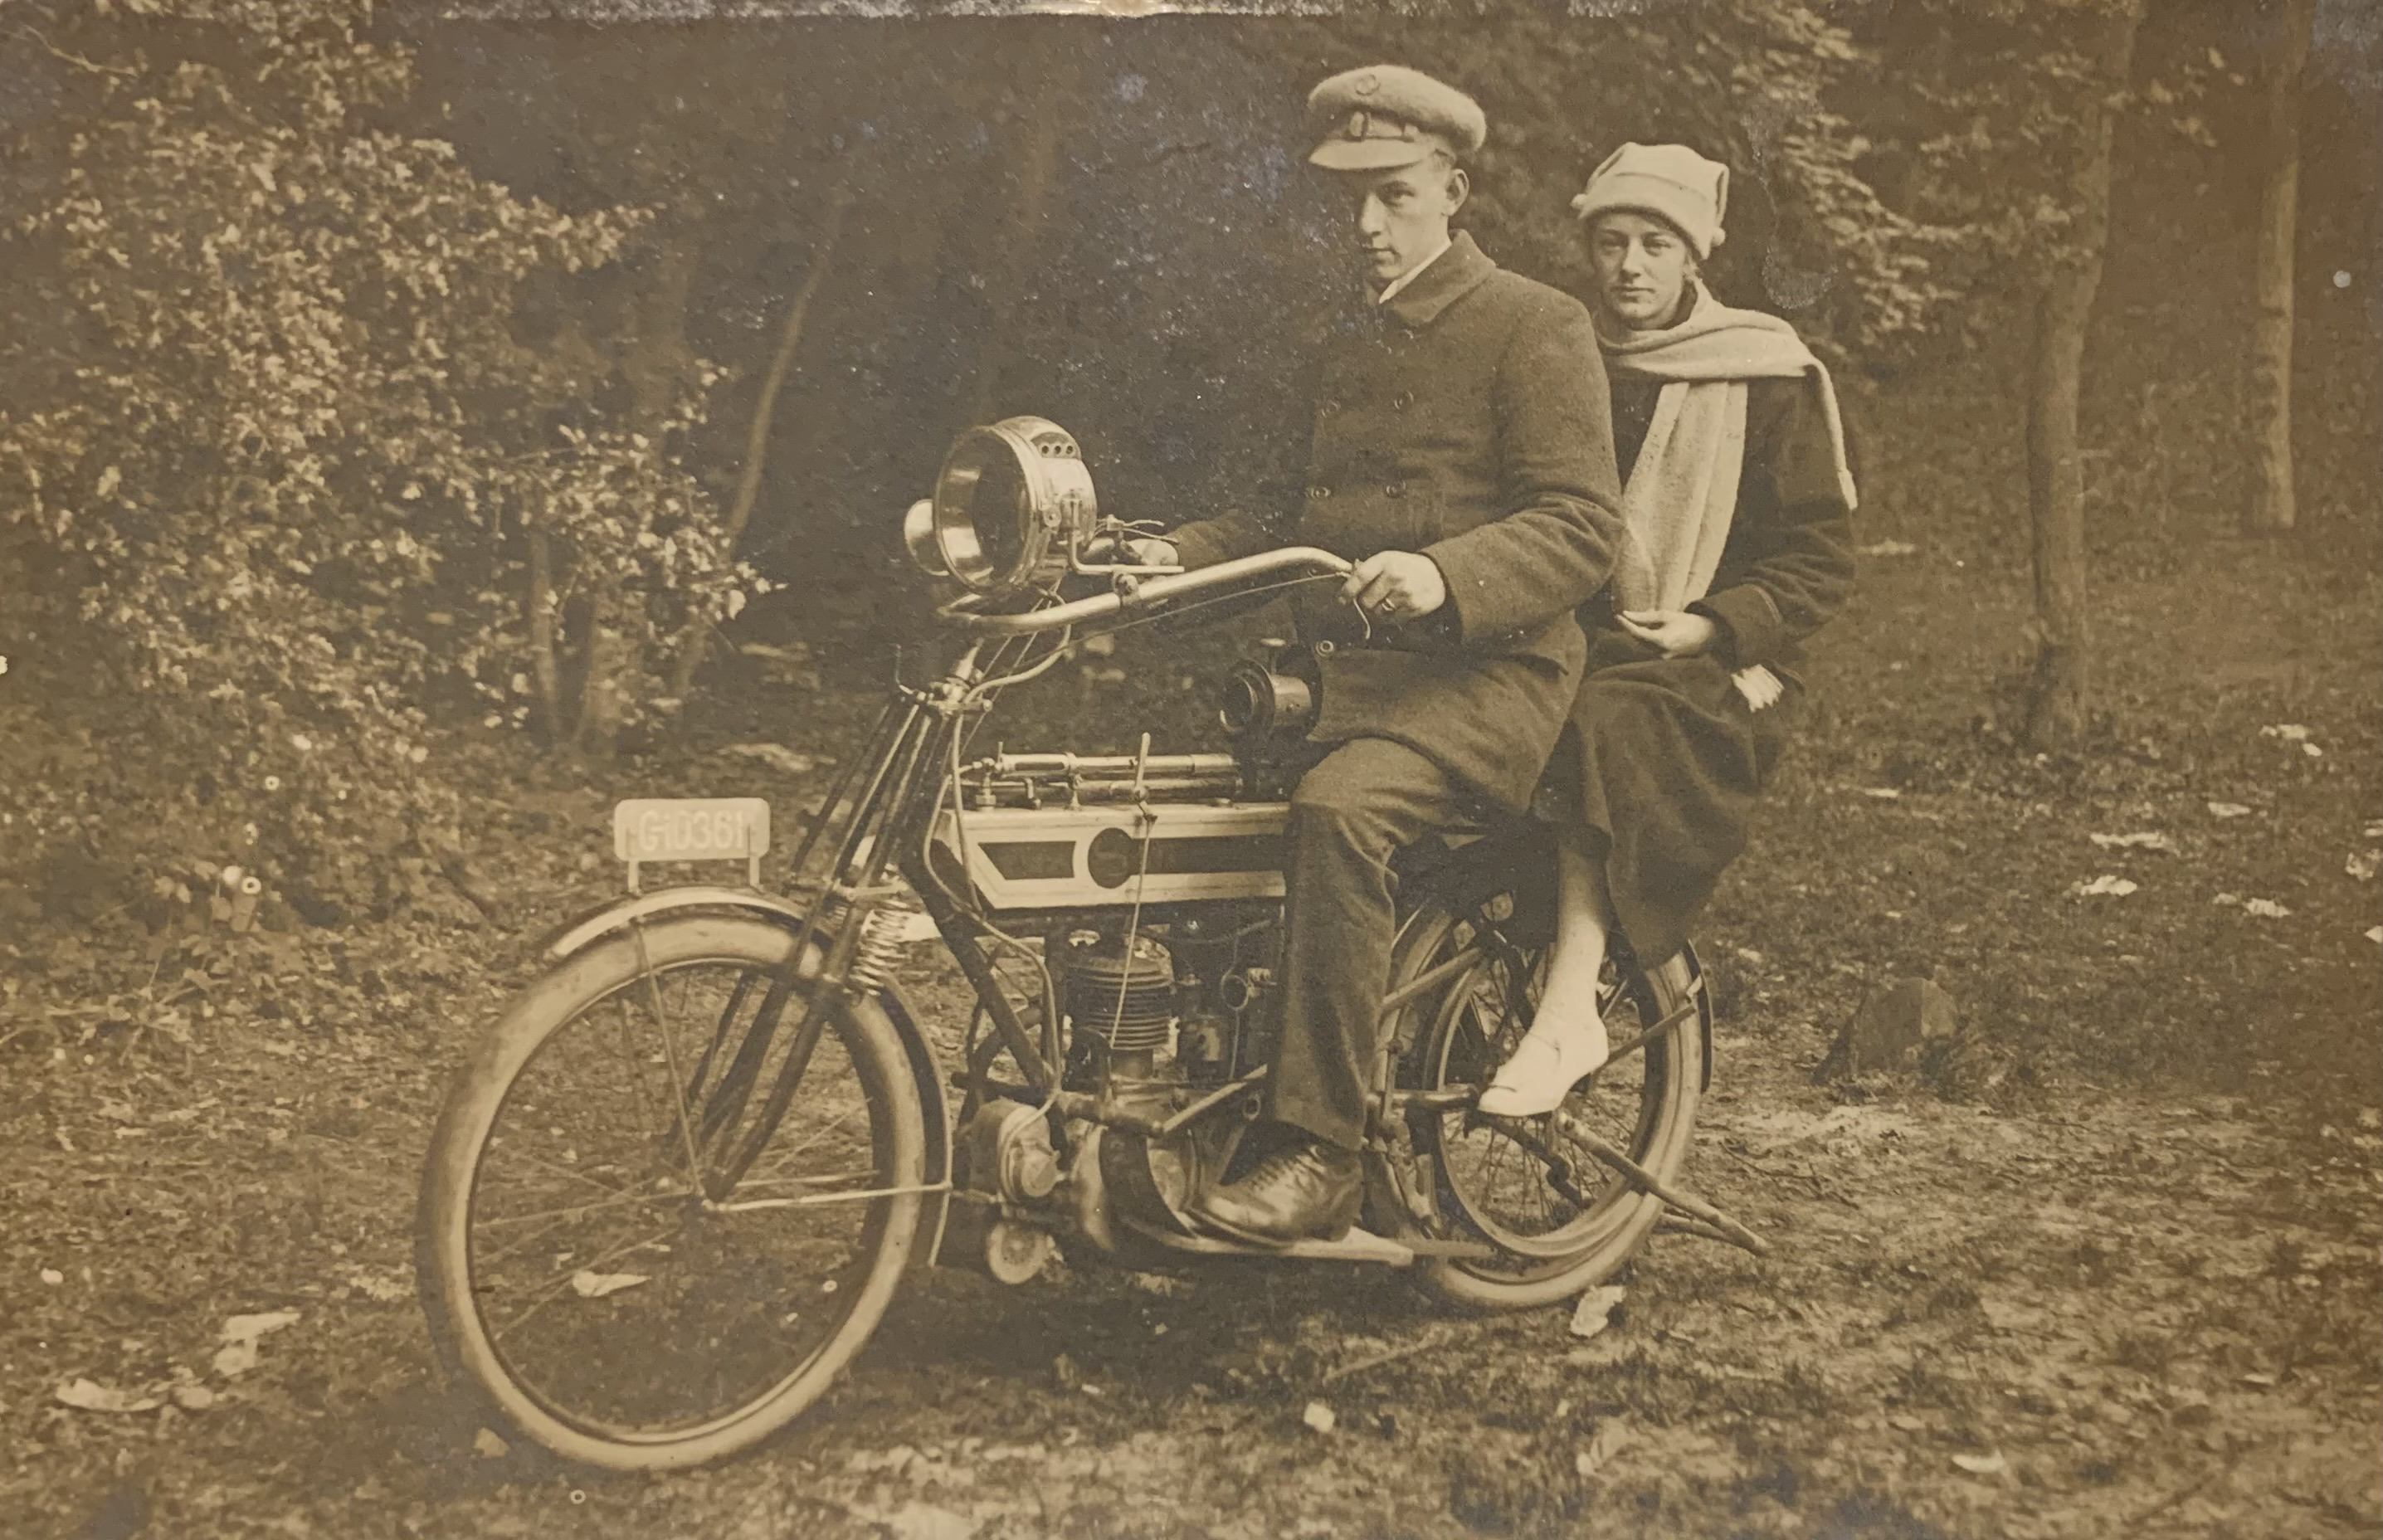
\includegraphics[width=1\textwidth]{boek_Tine_Blom.docx.tmp/word/media/image14.jpg}

\textit{Mijn ouders in hun verkeringstijd}

Mijn moeder was een Vlam uit Schoorldam. Zij had een broer Piet en een oudere zus, Hidda. 

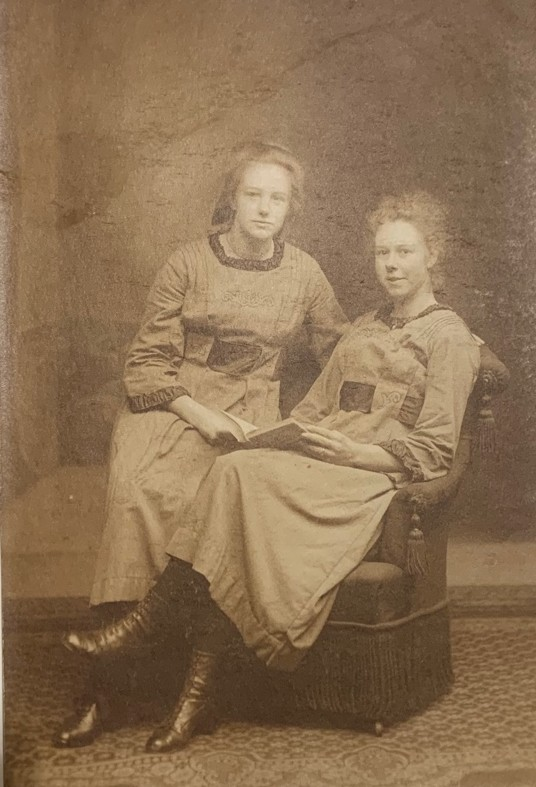
\includegraphics[width=1\textwidth]{boek_Tine_Blom.docx.tmp/word/media/image15.jpeg}
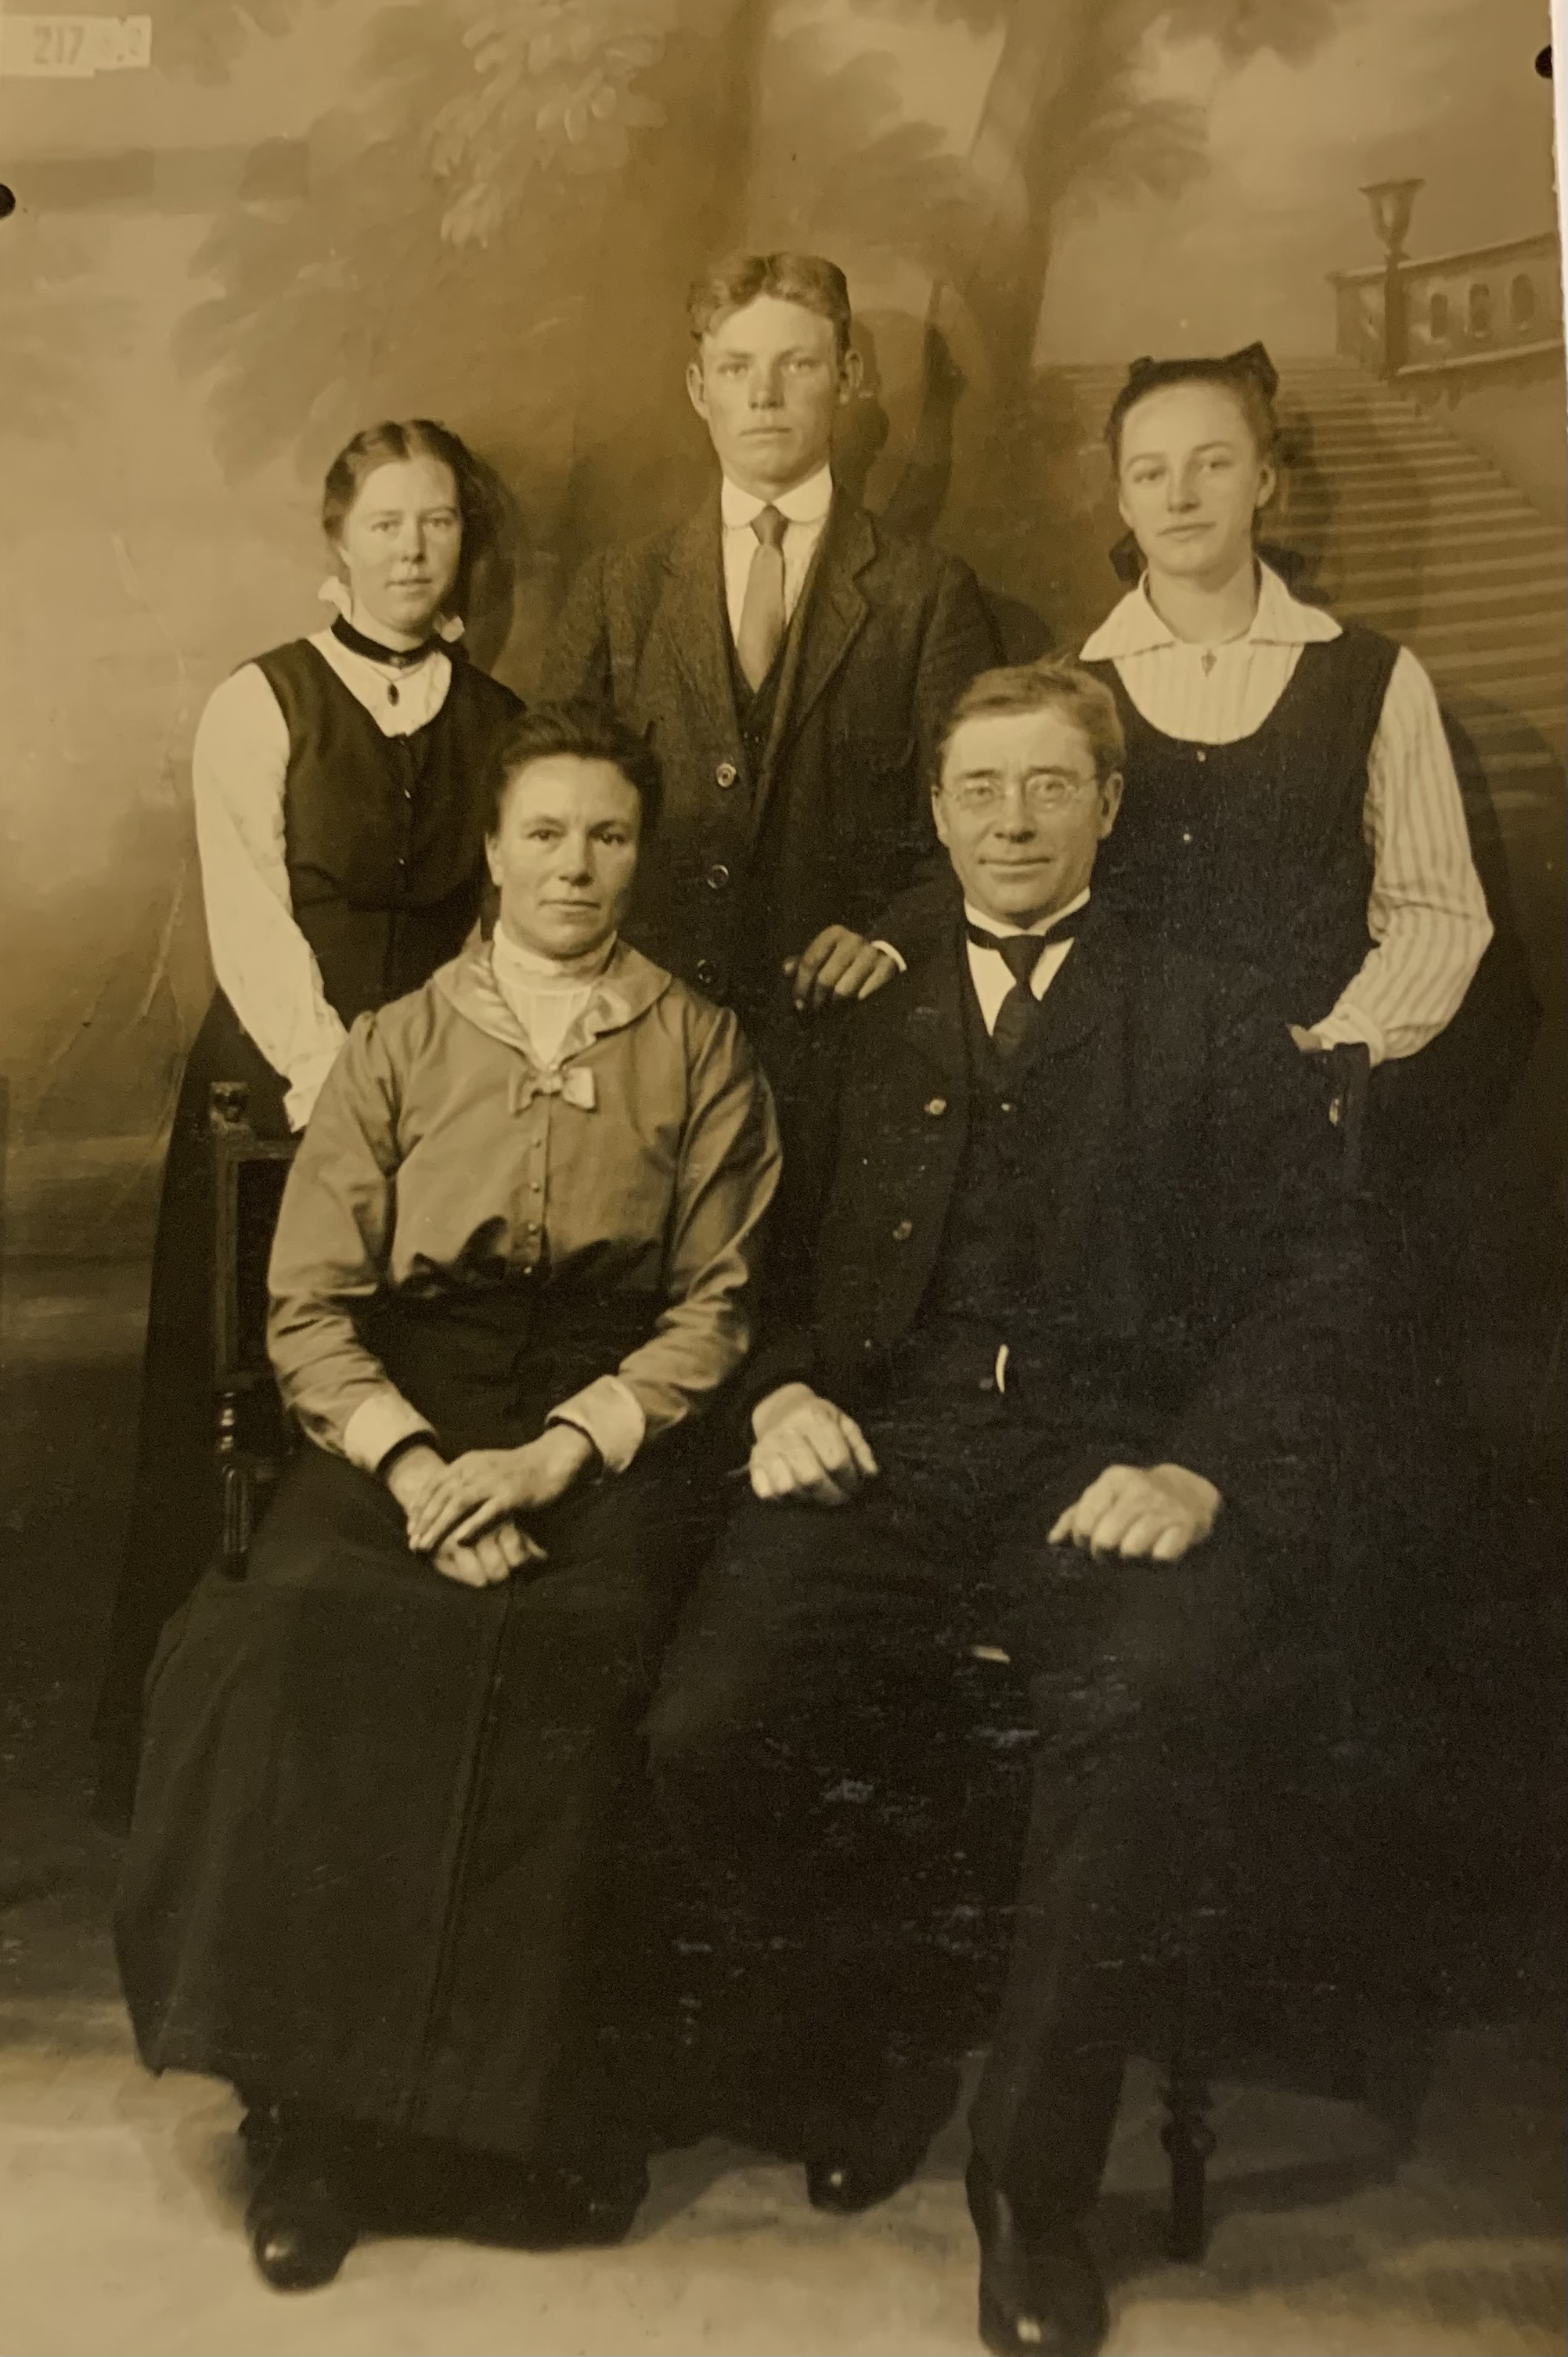
\includegraphics[width=1\textwidth]{boek_Tine_Blom.docx.tmp/word/media/image16.jpg} 

\textit{Mijn moeder (rechts) en haar zusje}  \textit{De familie Vlam (rechts achter mijn moeder)}

Mijn opa had samen met zijn niet getrouwde broer (ook weer een Piet) een boerderij. 

Mjn opa en oma woonden in een huis aan het Noord-Hollands kanaal. Broer Piet woonde op de boerderij. Voor die tijd was het een grote boer. Als je door het washok liep waren er links en recht stallen, en verderop stallen voor de paarden. En er liep ook een varken rond.

De ouders van mijn moeder hadden de scheepswerf op Schoorldam. Het was een gegoede familie. Later is die werf in handen gekomen van een andere familie. 

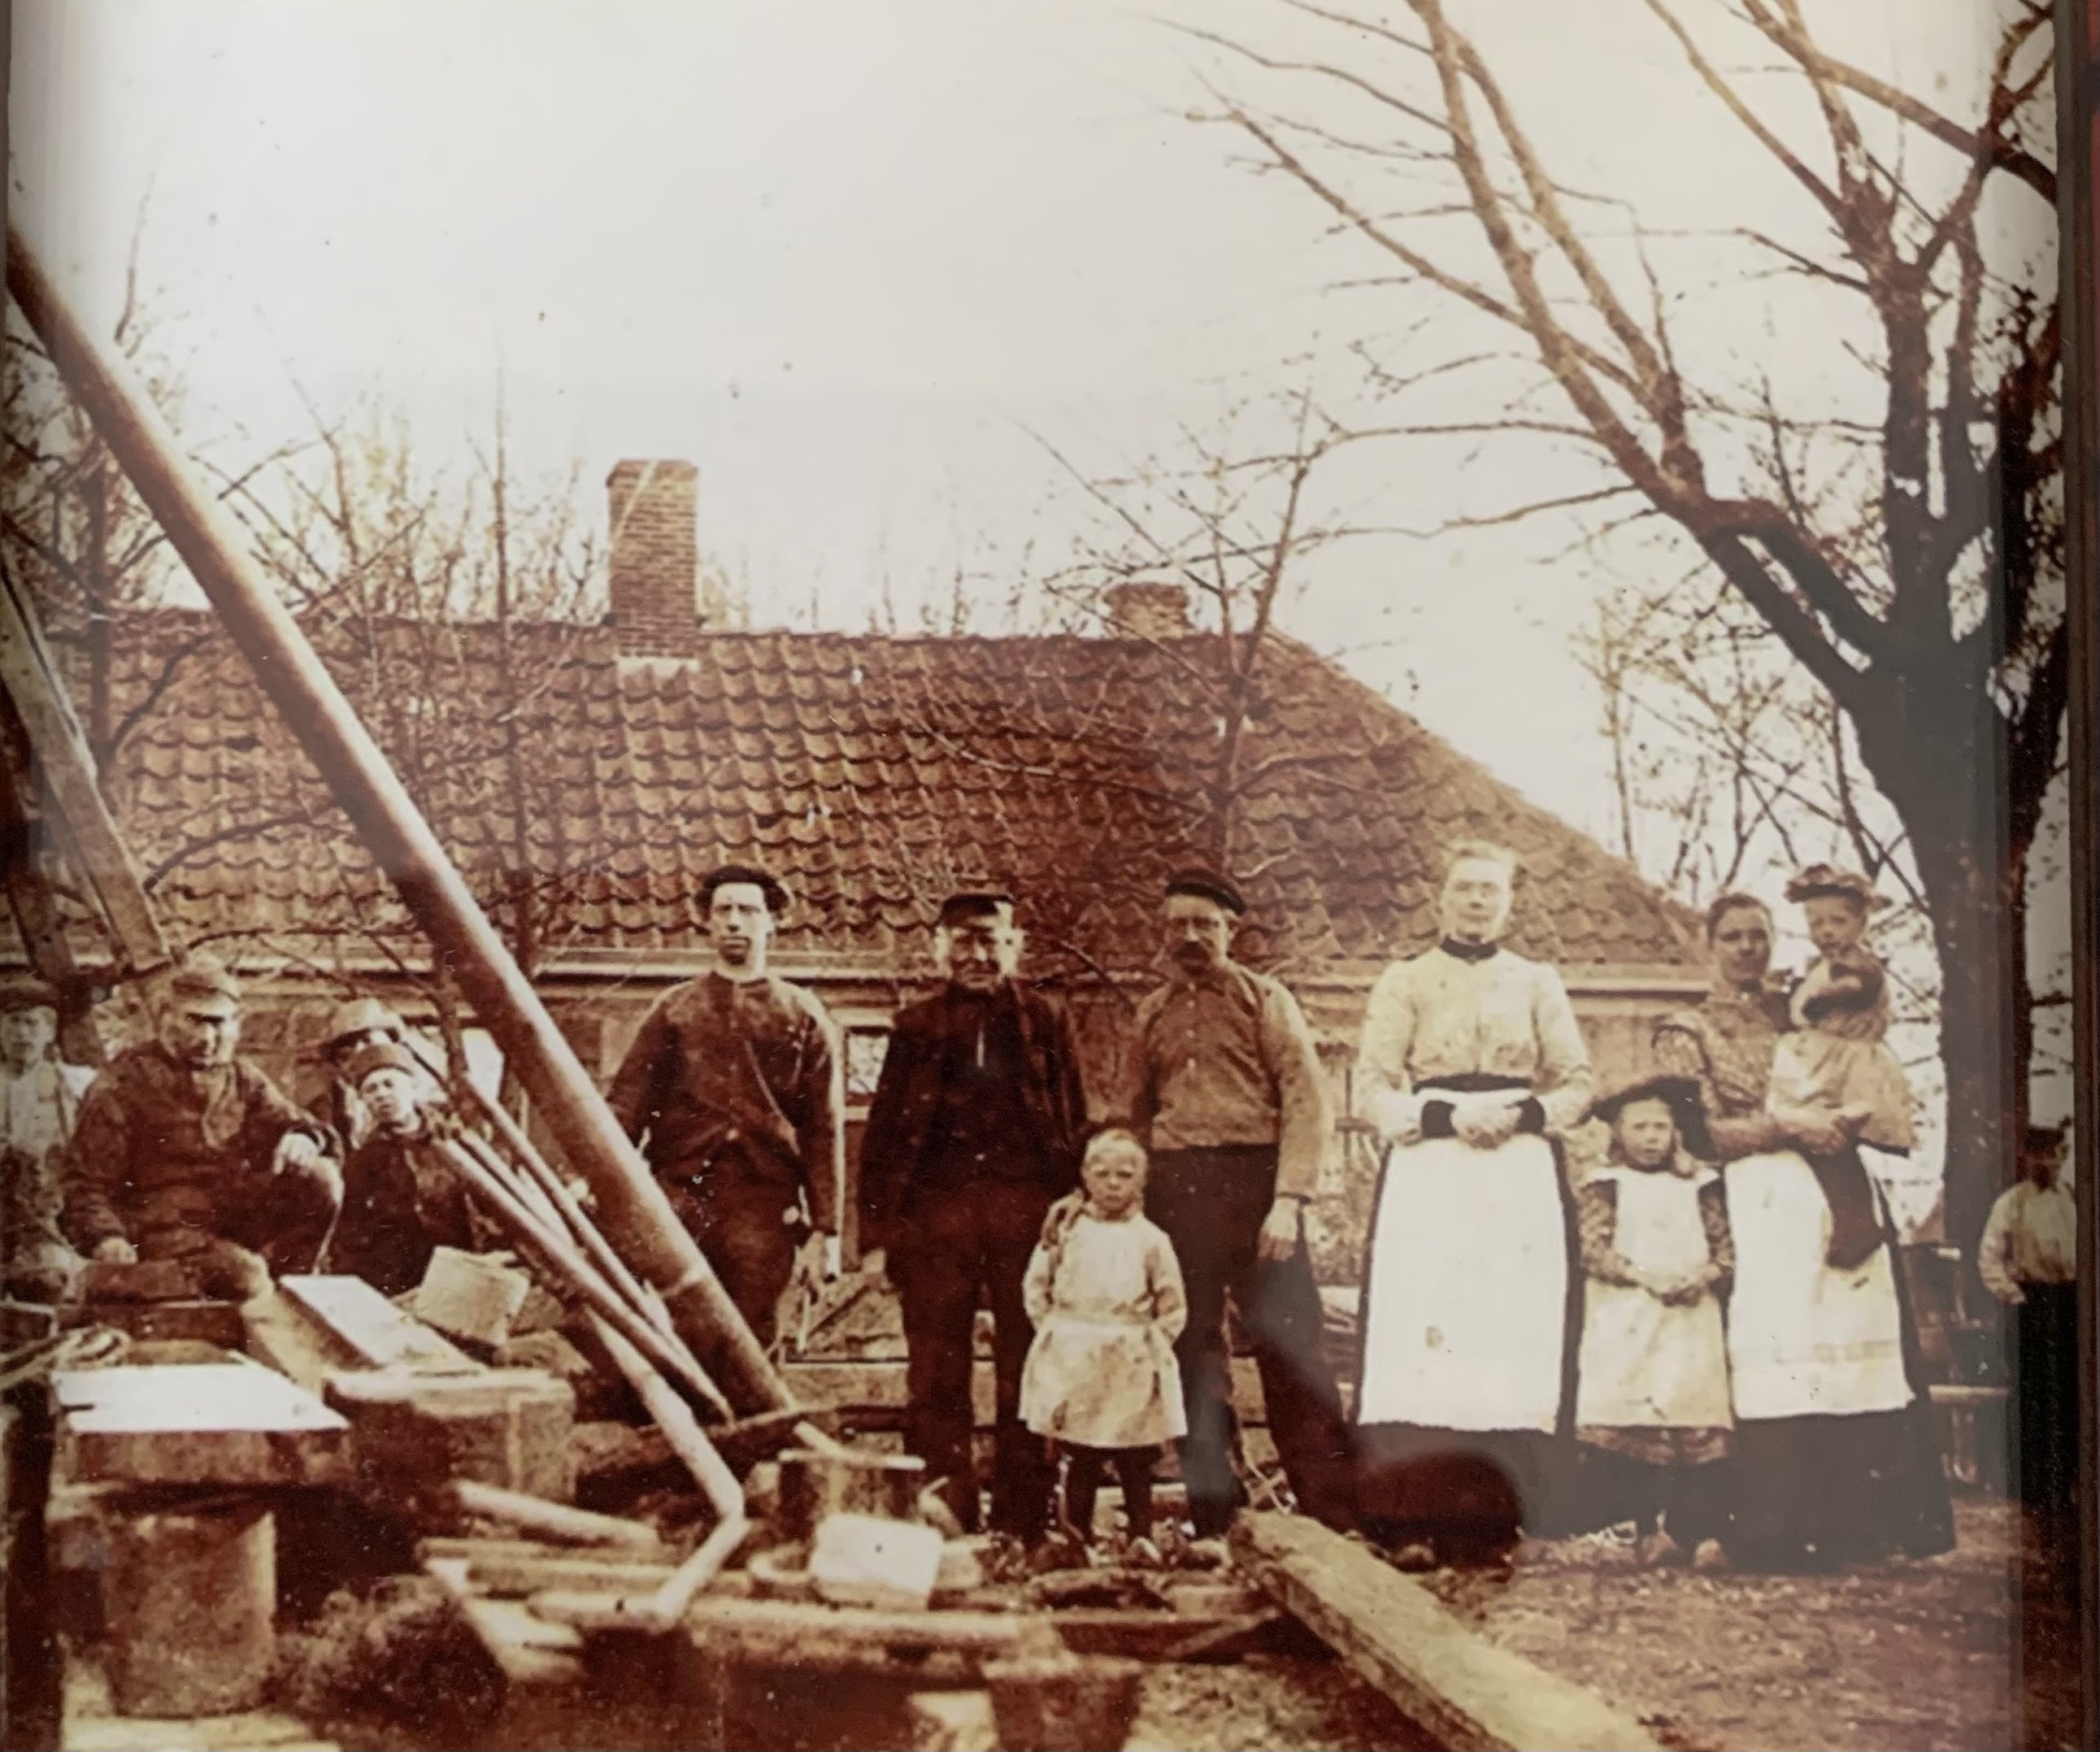
\includegraphics[width=1\textwidth]{boek_Tine_Blom.docx.tmp/word/media/image17.jpg}

\textit{Bij de werf. Rechts mijn oma met mijn moeder op de arm.}

De oma van mijn oma kwam uit Friesland, uit Kimswerd. Riemke Jans Westra heette ze, geboren in 1803. Van haar geboorte is de geboortelepel bewaard gebleven. 

Zij kwam met een dominee mee naar Noord-Holland voor een dienstbetrekking. Later heeft ze ook nog in het onderwijs gewerkt dus het moet een slimme vrouw zijn geweest. Ze is overleden in 1873.

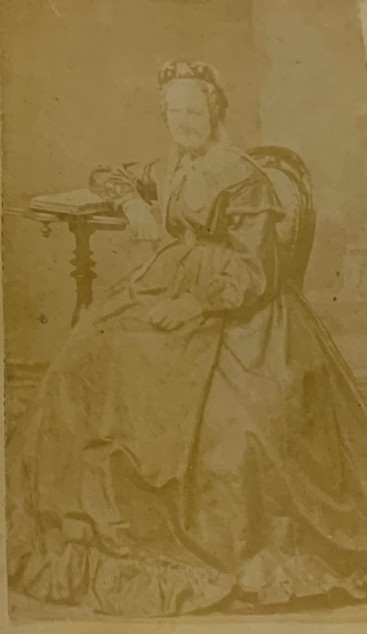
\includegraphics[width=1\textwidth]{boek_Tine_Blom.docx.tmp/word/media/image18.jpeg}

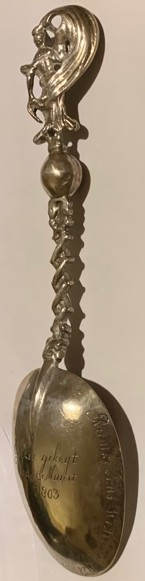
\includegraphics[width=1\textwidth]{boek_Tine_Blom.docx.tmp/word/media/image19.jpeg}\textit{Riemke Westra (geboren 1803) en de geboortelepel die voor haar gemaakt is. Op het ijs van de toen bevroren Zuiderzee gekocht. Dat staat als inscriptie op de lepel vermeld.}

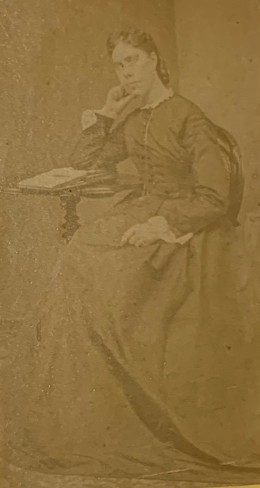
\includegraphics[width=1\textwidth]{boek_Tine_Blom.docx.tmp/word/media/image20.jpeg}

Haar dochter Hittje (die zich Aaltje noemde, ze vond Hittje zeker geen mooi naam; 1830-1950) heeft ook als onderwijzeres gewerkt.

\textit{Hittje (Aaltje) Westra} 

Ik heb een vriendin gehad die ook een Westra was, IJda Westra. Ze was in de verte familie. Haar vader was niet erg aardig voor haar. Haar moeder was wat ziekelijk en toen moest IJda alles maar overnemen. Als ze dan op school kwam had ze al weet ik hoeveel gedaan in het huishouden. Haar vader legde expres iets waar ze bang voor was in de kast waar zij dingen uit moest pakken.

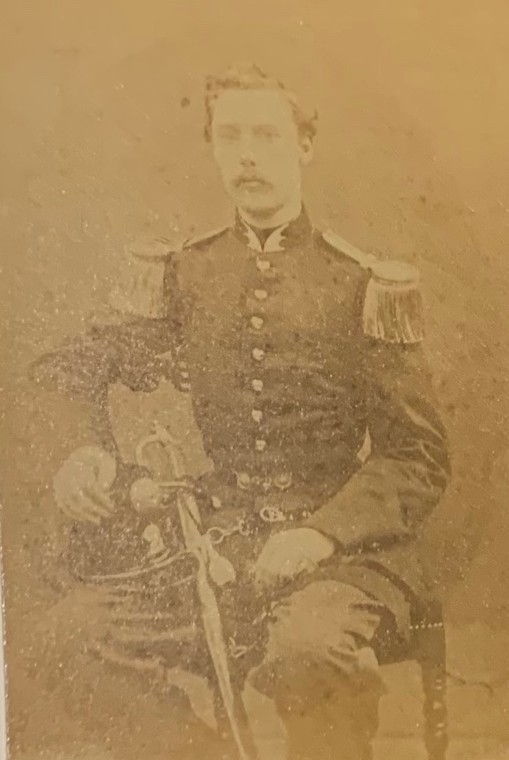
\includegraphics[width=1\textwidth]{boek_Tine_Blom.docx.tmp/word/media/image21.jpeg}In de familie zijn veel tekeningen bewaarde gebleven. Die zijn gemaakt door Jan Vlam (1833-1890), de broer van Hittje. Hij tekende op alles wat los en vast zat.

Onderstaand een tekening van zijn broertje Pieter (1828-1914) in de bedstee. Pieter was de opa van mijn moeder

\textit{Jan Vlam, de tekenaar}

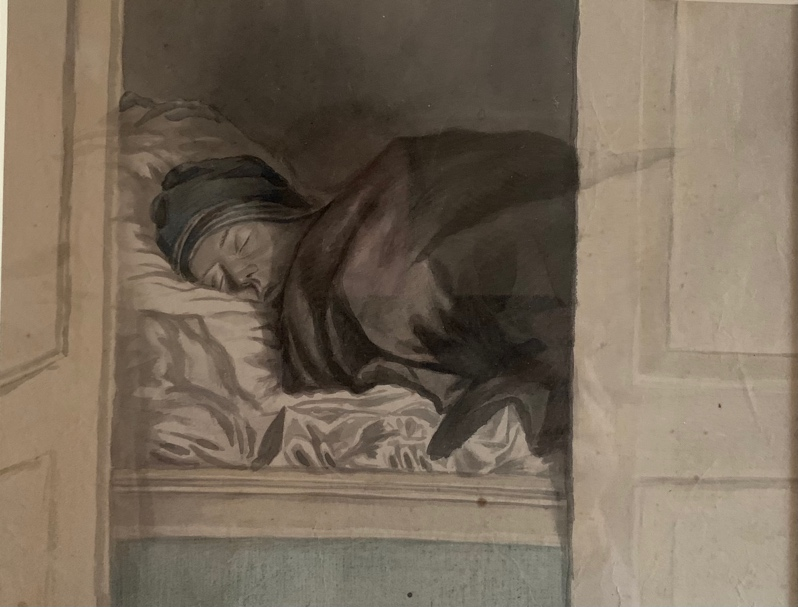
\includegraphics[width=1\textwidth]{boek_Tine_Blom.docx.tmp/word/media/image22.jpeg}

\chapter{\label{ref-004}Schoorl en Schoorldam  }

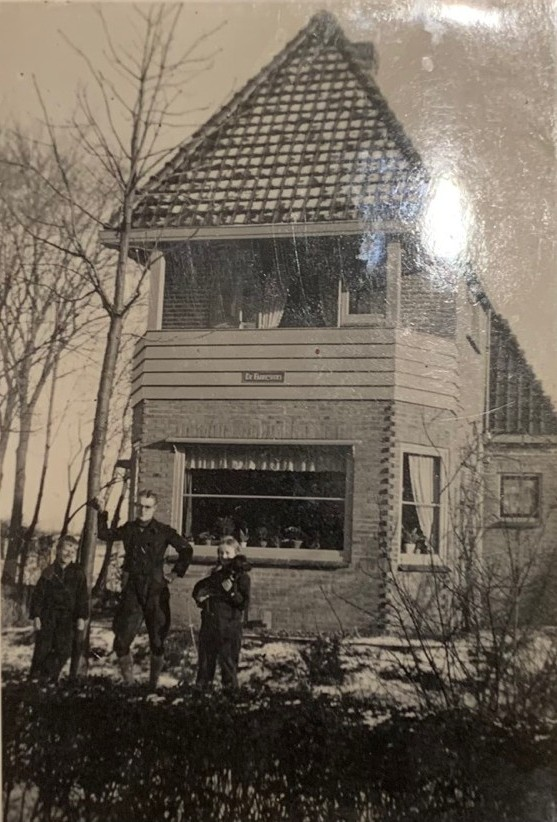
\includegraphics[width=1\textwidth]{boek_Tine_Blom.docx.tmp/word/media/image23.jpg}Toen ik 11 was zijn we naar Schoorl verhuisd. In december 1939. Vlak voor de Duitsers kwamen.

Wij vonden het wel leuk om naar Schoorl te verhuizen maar voor m’n vader was het niet zo leuk. Hij was maagpati\"{e}nt geworden en kon het bedrijf niet meer doen. Hij had last van maagbloedingen. 

Ik vond het leuk om het duin in te gaan.

In december zijn we er gaan wonen en in het voorjaar kwamen. Ik weet nog goed dat mijn vader en ik uit bed waren gegaan. Het wemelde toen van de vliegtuigen. Na 5 dagen gaf Nederland zich over. Toen kwamen er ook Duitsers in Schoorl. 

Ik herinner me dat opa Vlam vertelde dat hij met een Duitser had gepraat, dat was een boerenzoon, die moest in dienst. Dat was een goede Duitser zei opa. Die Duitsers zijn toen op de thee geweest. Toen zeiden wij dat moeten jullie maar niet meer doen.

Bert is toen ondergedoken. Eerst wisten we niet waar hij zat. Op een gegeven moment was hij 

\textit{Het huis in Schoorl  }



  

ondergedoken in Noord-Holland. Toen zijn mijn moeder en tante Hidda op de fiets bij hem langs geweest. Bert kon daarna vrijstelling krijgen als hij aan de landbouwhogeschool ging studeren in Groningen. Daar heeft hij de oorlogsjaren op gezeten. 

Voor mij ging de school al die jaren gewoon door. Ik ging meestal met de fiets naar school.

Maar soms met de bus. Achter de bus zat een apart karretje dat stookten ze op turf en daar reed de bus op. Er zaten soms ook gewoon Duitsers in die keurig een kaartje kochten. Ik deed de huishoudkundige opleiding maar de laatste winter was er niks meer om mee te koken en ging de school ook dicht.

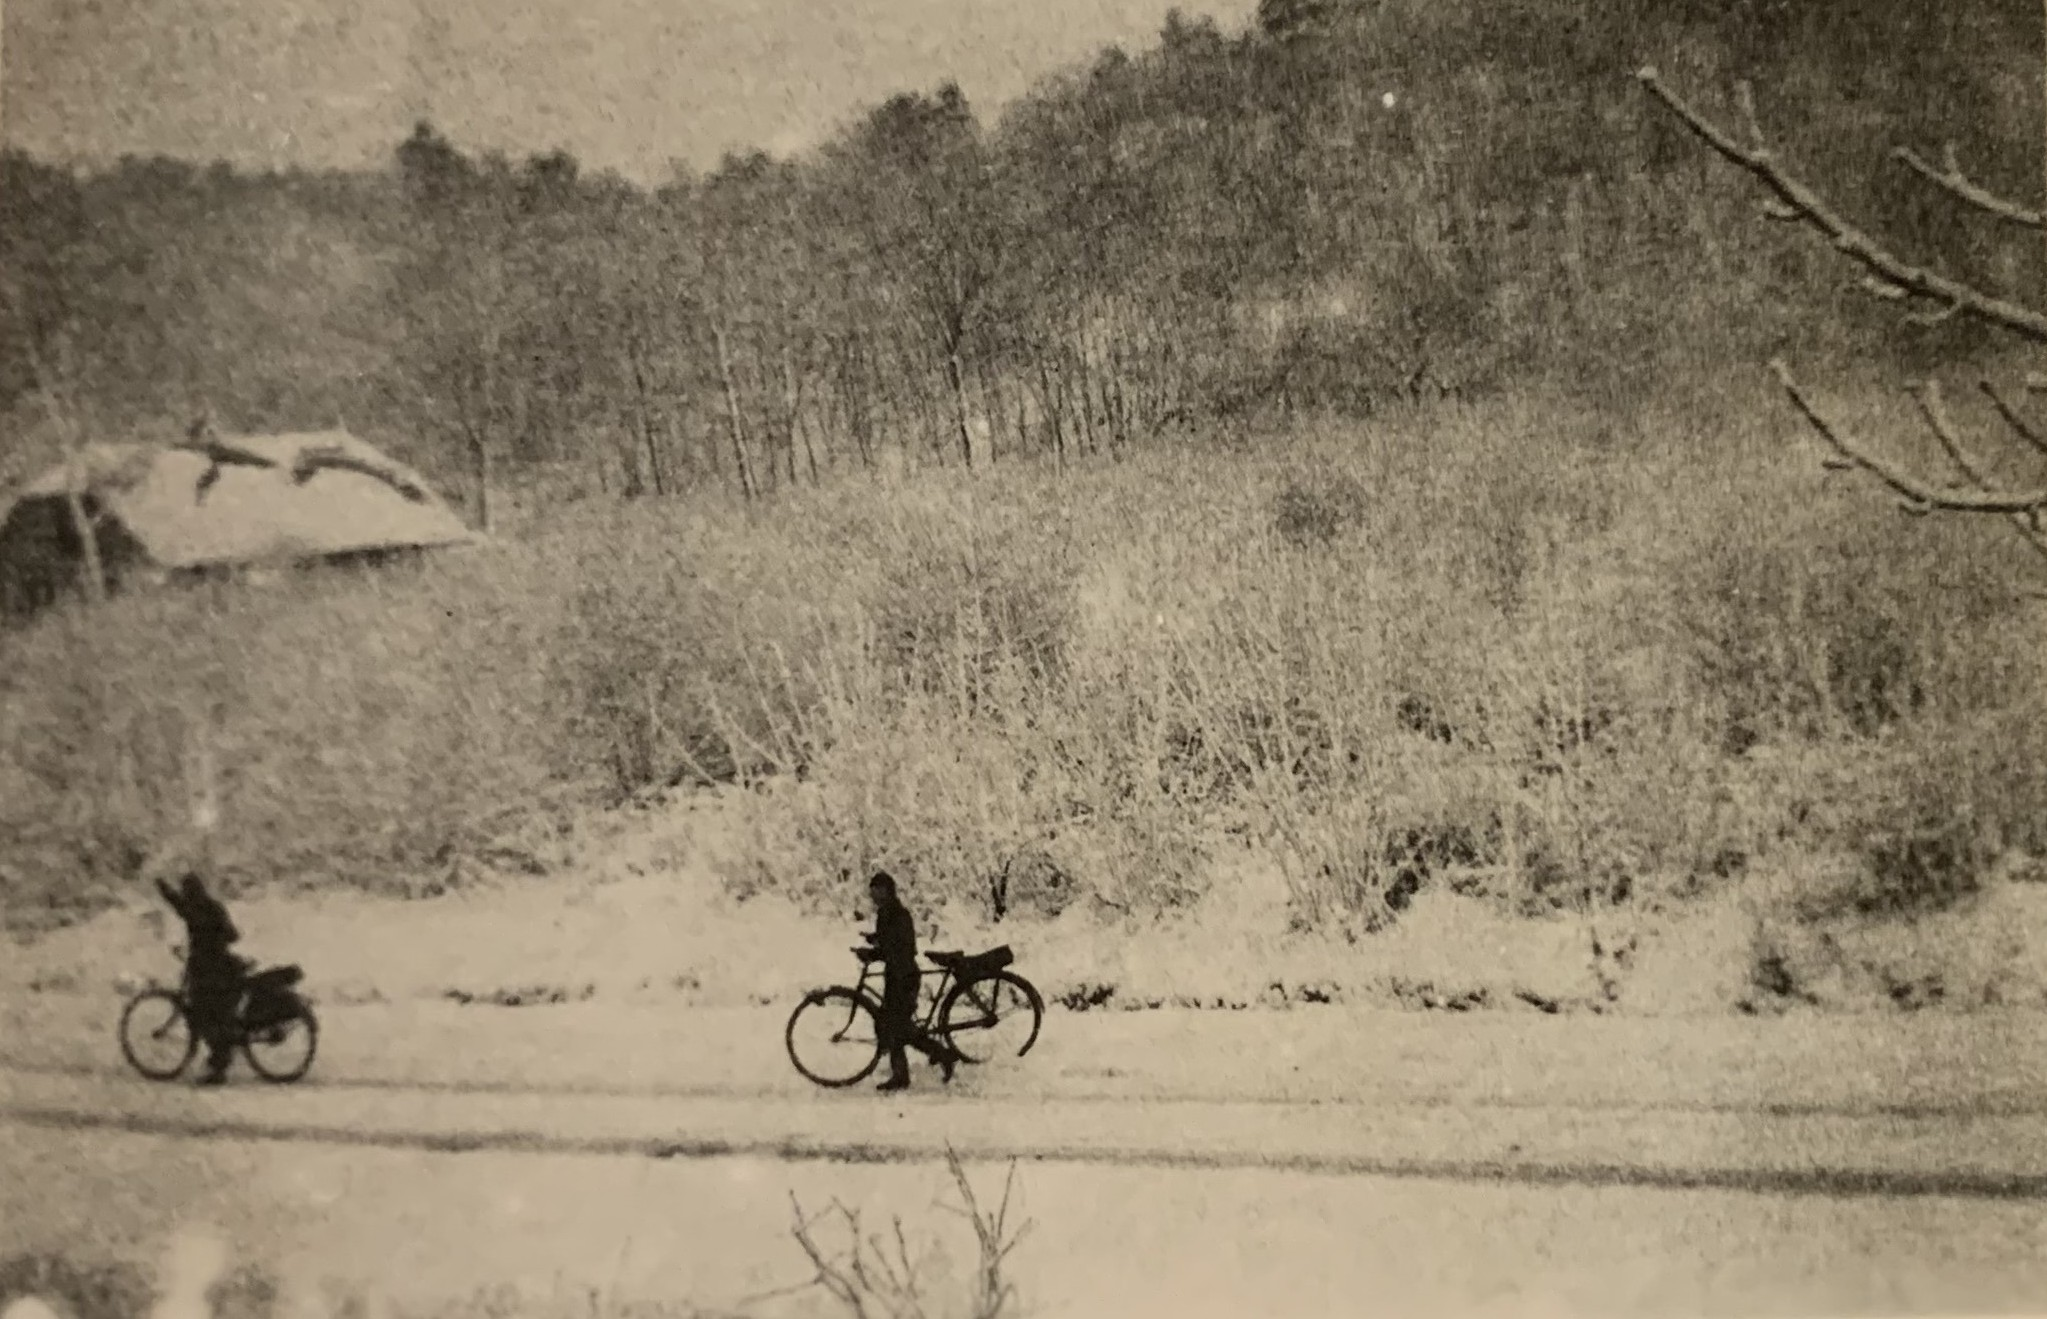
\includegraphics[width=1\textwidth]{boek_Tine_Blom.docx.tmp/word/media/image24.jpg}

\textit{Kees en Tine gaan op de fiets naar school}

Soms als we naar school moesten fietsen lag er heel veel sneeuw. Dat werd toen natuurlijk niet opgeruimd alleen maar platgereden.

Aan het eind van de oorlog moesten we evacueren. Want ze waren bang voor landingen via het strand en collaboratie. Toen gingen we naar Schoorldam. Dat was heel gezellig. Bij opa en oma. Eerst sliep ik met Kees op zolder. Maar op een geven moment bleef tante Hidda op de boerderij en toen mocht ik in tante Hidda’s slaapkamer. Voor ons kinderen was het allemaal niet zo erg. In die tijd was er geen elektriciteit en werd de stal tijdens het melken verlicht met olielampjes. De reden was niet leuk maar het zag er zo gezellig uit!

\textit{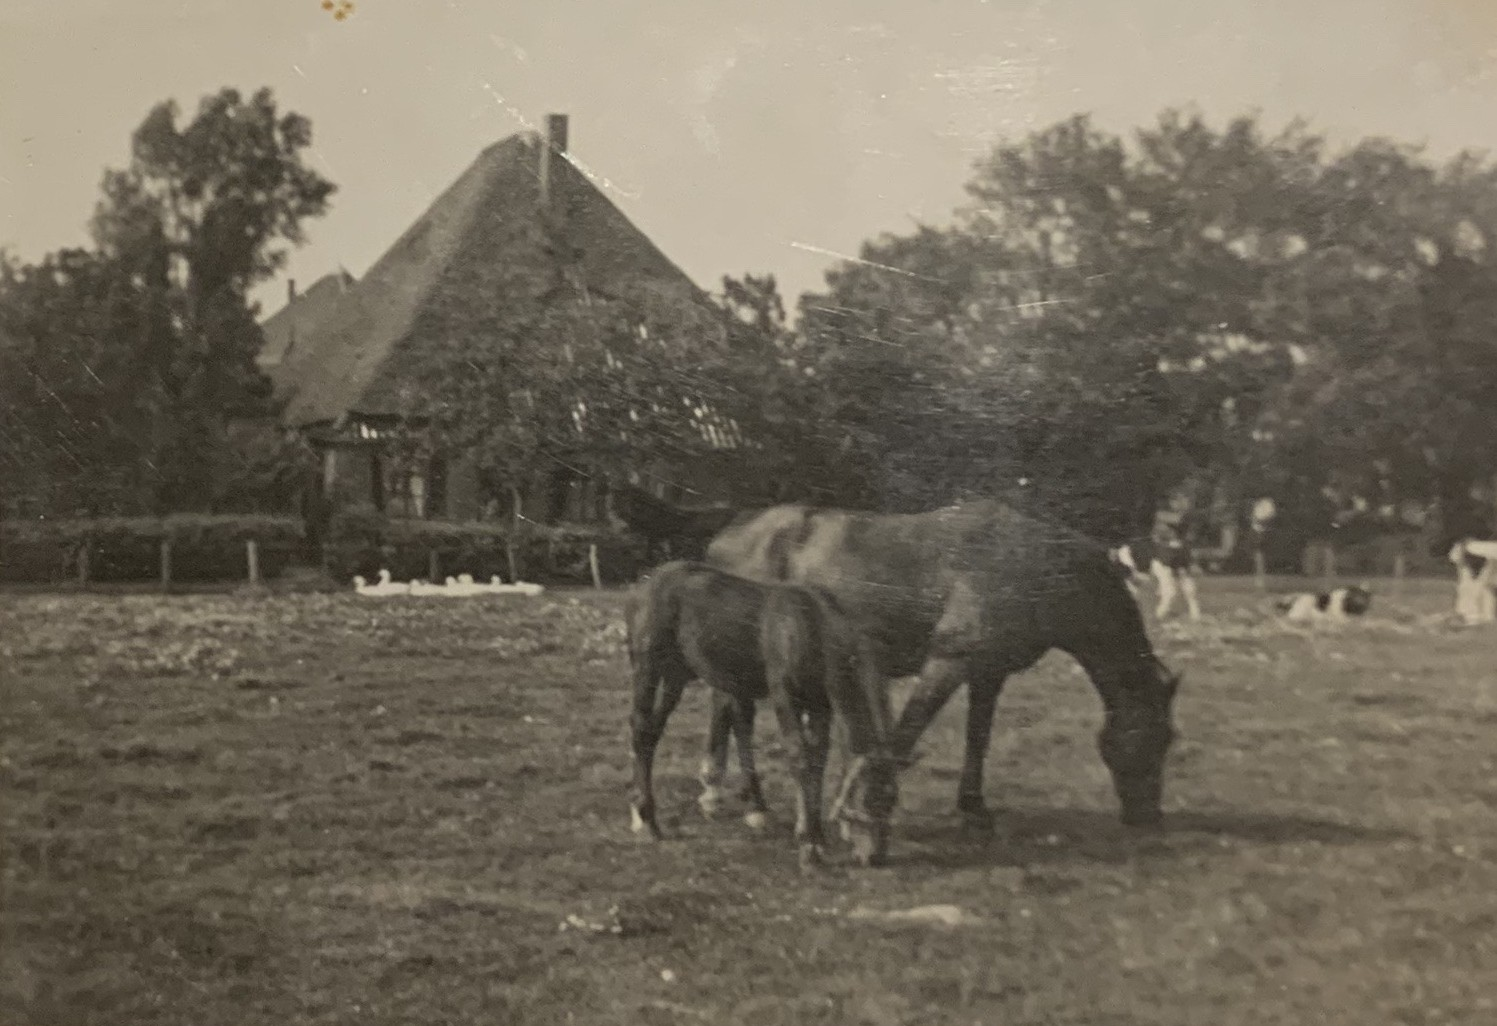
\includegraphics[width=1\textwidth]{boek_Tine_Blom.docx.tmp/word/media/image25.jpg}}

\textit{De boerderij op Schoorldam }



Mijn vader was gewoon thuis. Eens kwamen er ’s avonds een paar Duitse militairen in vol uniform en werd hij gecharterd om aan de Atlantikwall te werken. Hij moest daarbij helpen. Hij heeft er reuzepret gehad. Ze maakten alles zo langzaam en slecht mogelijk. 

Ook mijn beide opa’s konden gewoon thuis blijven, want ze hadden nuttige beroepen. De ene was boer op Schoorldam en de ander smid in Oudkarspel. 

Op een gegeven moment zei opa we gaan weer terug naar Schoorl. Eigenlijk mocht dat nog niet. Dat was voor de bevrijding maar de Duitsers waren al haast verslagen en ze lieten ons met rust toen we naar huis gingen.

Toen kwam de bevrijding. Dat hoorden we op de radio! Toen was iedereen blij en vrolijk. En moesten we allemaal weer een beetje de draad oppakken. 

In de oorlog was het een beetje saai. Er was helemaal niks te doen. Alles was dicht of verboden. Het enige wat er nog was de KJVO. De Kennemer jeugdgroep voor onthouders. Dat was opgezet door een leraar van de MULO. 

Dat was heel gezellig. Er werd elke week een gezellige avond georganiseerd met een lezing of we deden zelf dingen. En we zongen ook. In de winter hadden we dan een zangavond. En er werd toneel gespeeld.

We gingen kamperen met de KJVO op de Veluwe bij Doornspeijk. Dan gingen we om 4 uur s ochtend op de fiets van Schoorl naar Amsterdam om de eerste boot naar de Veluwe vanaf Amsterdam naar Harderwijk te kunnen pakken. En dan weer fietsten we daarna van Harderwijk naar Doornspeijk. We siepen in schaapskooien. Eentje voor de jongens en eentje voor ons. Dat was heel gezellig. Schuil organiseerde dat allemaal. Hij kende daar boeren. Je kon je bij de pomp wassen met koud water. Er was geen toilet maar een kuil buiten in het bos. Dat ging ook best. We wandelden en fietsen veel. Dankzij opa hadden wij ook fietsen. Er was ook een Joodse jongen mee die eigenlijk was ondergedoken. Dat vond ik altijd wel eng als we Duitsers tegenkwamen maar het is gelukkig allemaal goed gegaan. 

\chapter{\label{ref-005}\textit{Tine en Kees, schoolfoto 1938-1939 }



 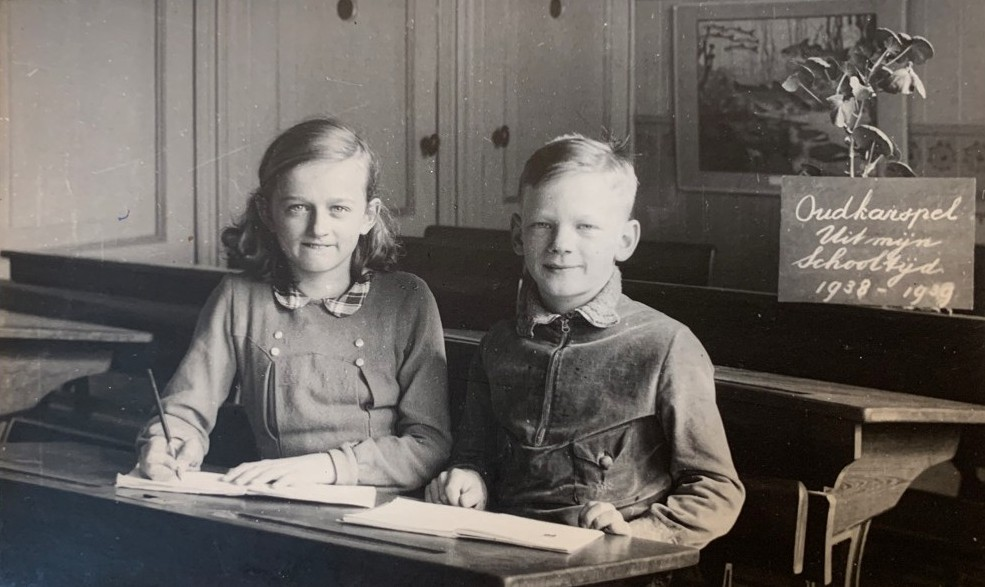
\includegraphics[width=1\textwidth]{boek_Tine_Blom.docx.tmp/word/media/image26.jpg}
 
 \section{Opleiding}

Het grootste gedeelte van mijn basisschooltijd woonde ik in Oudkarspel. Toen was het zo dat je niet naar de kleuterschool ging, school begon toen je 6 jaar oud was. Ik ben naar een openbare lagere school gegaan, het was de enige school in het dorp, mijn vader had ook op deze school gezeten. Naar mijn idee was het een hele grote school met veel ruimte om te spelen. Er was ook een waterput, mijn vader vertelde dat hij als kind daar altijd overheen sprong, dat was een spelletje. Ik kon me dat niet zo goed voorstellen hoe dat dan moest. Van de lagere school kan ik me herinneren dat de eerste en de tweede klas in hetzelfde lokaal 

zaten en ik altijd naar 

het bord van de tweede klas zat te kijken. Lezen kon ik eigenlijk al voordat ik naar school ging en daarom vond ik het in eerste klas een beetje saai. Rekenen vond ik niet zo leuk, ik was meer van de talige vakken en aardrijkskunde en geschiedenis. Op school zat ik veel te lachen. Ik zat meestal naast een vriendin met wie ik altijd aan het giebelen was, hierdoor werden we een keer uit elkaar gehaald en moesten we beide in aan de andere kant van het lokaal zitten. Ik vond het leuk om naar school te gaan. We gingen lopend en ik nam vaak mijn (ijzeren) hoepel mee, hier sloeg je tegenaan met een stok zodat ie ging rollen. Als de bel ging dat stond je allemaal voor de klas in de rij te wachten totdat de juf of meester je naar binnen liet. In die tijd gingen veel kinderen met klompen naar school, hier stond dan een bak voor klaar in het schoolgebouw. Ik had meestal geen klompen aan omdat ik ze niet prettig vond zitten. In 1939 zijn we naar Schoorl verhuisd, hier heb de 6\textsuperscript{e} klas van de lagere school gevolgd. In Schoorl zat ik op een geheel nieuwe school. Ik kan me nog herinneren dat ze daar rekenboekjes hadden met de antwoorden achterop, zodat je kon controleren of je het antwoord goed had: (lachend) Ik controleerde heel veel. Ik vond het verhuizen naar Schoorl niet zo erg, ik vond het daar veel leuker dan in Oudkarspel vanwege de duinen en het strand. Tijdens de bezetting mochten we alleen niet naar het strand, voor het geval de Engelsen kwamen. 

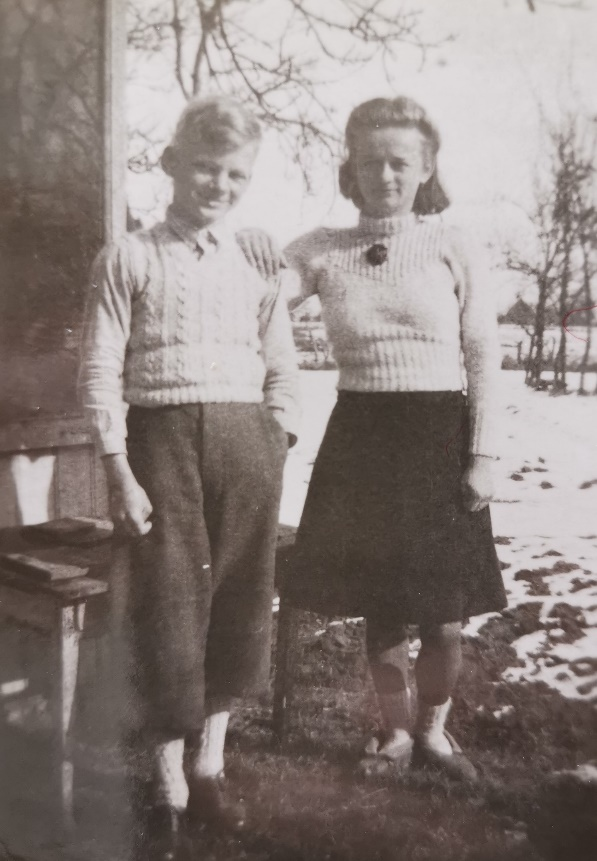
\includegraphics[width=1\textwidth]{boek_Tine_Blom.docx.tmp/word/media/image27.jpeg}

\textit{Tine en Kees }



Na de basisschool ben ik naar de Mulo in Bergen gegaan, dit was een opleiding van 4 jaar. Het was toen oorlog dus ik heb deze school nooit van binnen gezien. In het schoolgebouw zaten de Duitsers dus daar konden we niet meer zijn. We zaten toen tijdelijk in een ander schoolgebouw. Ik kan me herinneren dat er dat er eens Duitsers op dat schoolplein aan het oefenen waren, de meester heeft ze toen uitgelegd dat het voor te veel afleiding zorgde voor de leerlingen en waarachtig hoor, ze gingen weg. Ik weet nog dat we dat geweldig vonden.

Op een gegeven moment ben ik gestopt met die school want toen lagen we vaker in de berm vanwege de beschietingen door de geallieerden dan dat we in de klas zaten. Pas na de bevrijding heb ik het afgemaakt.

Na de Mulo ben ik naar huishoudschool in Alkmaar gegaan om de huishoudkundige opleiding te volgen. Hier werd je opgeleid tot leidinggevende van bijvoorbeeld het schoonmaakpersoneel in een instelling. Dit was een tweejarige opleiding. Ik moest dan ‘s morgens met de bus (die heel vol was, ook met Duitsers) die gestookt werd met hout. Er hing dan een karretje achter de bus waar dit gestookt werd zodat de bus kon blijven rijden, vanwege de oorlog was er geen benzine meer. Ik moest dan vroeg opstaan en ik was niet zo van het ‘’leuk vroeg opstaan’’ maar je deed het gewoon, dit was nou eenmaal zo. 

Bert had wel verder kunnen gaan studeren. Dat wou m’n vader graag. Bert wou dat niet; hij wou trouwen! Na de oorlog zijn ze getrouwd vlak voordat ik naar Engeland ging.

Werken in het Wilhelmina Gasthuis

Ik ben tot mijn 19\textsuperscript{e} naar school gegaan. Hierna heb ik even in Bergen gewerkt in een huis waar groepen jongeren kwamen voor lezingen en studie (voor als je dominee wil worden) in de grote keuken gewerkt. Ik kookte dan samen met een paar kinderen voor deze groepen en ik regelde de bestellingen. 

\chapter{\label{ref-006}London}

In 1948 ben ik naar Londen vertrokken, ik was toen 20. In de oorlog kon je niks. En toen las ik eens een keer iets over Londen. En toen dacht ik. Als het weer vrede is dan wil ik naar Londen! Dat leek me zo enig! 

Een poos daarvoor heeft een meisje uit Londen bij ons een uitwisseling gedaan. Ze is toen veertien dagen blijven logeren. Via haar heb ik destijds het adres van een gezin in Walton on Thames gekregen. Dit meisje, een kraamverzorgster, heeft daar nog een goed woordje voor me gedaan. Ik weet alleen niet meer hoe ze heette. Na een briefwisseling mocht ik bij het gezin aan de slag als hulp in de huishouding. 

Mijn doel was om mijn Engels te verbeteren. Voordat ik naar Londen ging was mijn Engels al best goed. Maar toch wilde ik graag nog beter worden zodat ik het wat makkelijker zou kunnen spreken. Jaa, want ik wilde in eerste instantie eigenlijk stewardess worden! Maar helaas is dat nooit gebeurd hoor. Haha. 

\textit{Op Trafalqar square.    }



 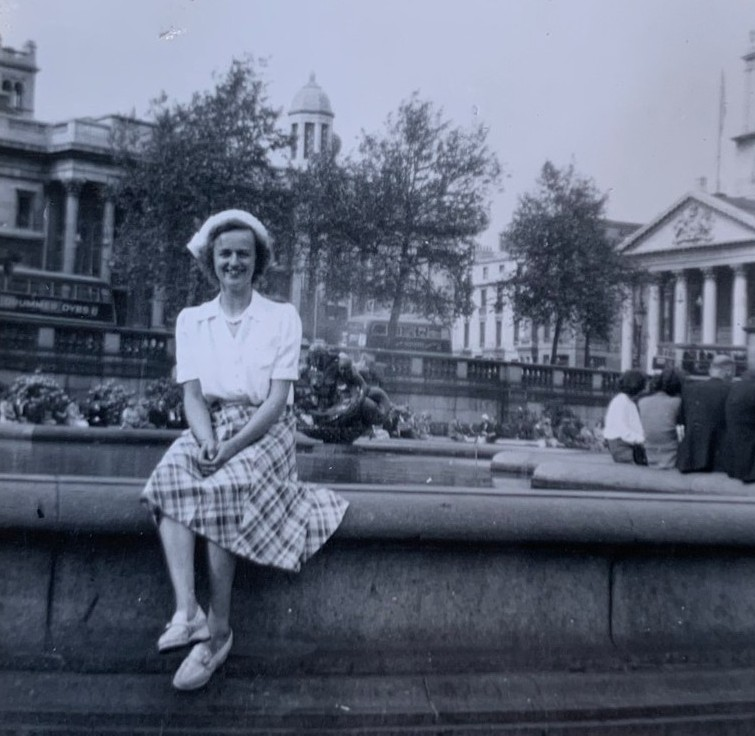
\includegraphics[width=1\textwidth]{boek_Tine_Blom.docx.tmp/word/media/image28.jpg}

Dit was mijn eerste grote reis. In de oorlog mocht je namelijk het land helemaal niet uit.

Mijn vader en moeder lieten het door de vingers dat ik zo ver van huis wilde. ‘’Als je dit echt wil, zullen wij je niet tegenhouden’’ zeiden ze. Ze vonden het best. 

Voor ik naar London ging had ik al een foto gezien van Trafalgar square. Ik vond dat echt London! En ik had toen al bedacht dat ik daar op de foto wou.

Mijn broer Kees heeft me destijds naar de boot gebracht in Hoek van Holland. Vroeg in de ochtend gingen we samen met de trein. Maar eenmaal bij de douane mocht ik de boot helemaal niet op. Ik werd tegengehouden omdat ik geen werkvergunning had. Dit wist ik of het gezin waar ik zou komen te werken van tevoren helemaal niet. Het was een hele bedoening en de politie kwam er zelfs bij. Een vriendelijke Nederlandse jongen schoot me te hulp en na heel wat telefoontjes, tevergeefs vertrok de boot uiteindelijk zonder mij. Dus kon ik weer terug naar huis!

Na een lange reis kwam ik s’ avonds laat weer thuis aan. Het was al lang donker toen ik op de deur klopte. Mijn vader deed de deur open: ‘’Dag mevrouw’’ zei mijn vader. Want hij herkende me helemaal niet. Ik zei: ‘’Hallooo, hier ben ik weer!’’ Ik had ze van te voren niet gebeld, want dan zouden ze zich daar alleen maar druk over maken. 

Na een briefwisseling met het gezin uit ‘Walton on Thames’, bellen met Engeland dat was veel te duur, was een werkvergunning alsnog zo geregeld en kon ik de keer daarna zo de douane door. 

 

Na aankomst in Engeland werd ik door de heer des huizes ‘Gerald Wilson’ opgehaald. Eerst gingen we naar het politiebureau om de ‘working permit’ te checken. Dat moest toen nog.

Gerald Wilson, werkte oorspronkelijk bij de marine, in een basis in Hong Kong, hij is toen gevangengenomen door de Japanners en in een concentratiekamp terechtgekomen. Gelukkig heeft hij het overleefd en na de oorlog werkte hij als ingenieur. Hij moest toen niets meer te maken hebben met alles wat maar uit Japan kwam.

De vrouw heette: Dorothy (Kitching?) Toen ik daar aan kwam hadden ze twee meisjes. Jillian en Judith. Jillian was de oudste. Aan het einde van het jaar dat ik er was bleek Dorothy in verwachting van een derde kind. Dit werd een jongetje. (John) En daarna toen ik weer terug in Nederland was hebben ze nog een zoon gekregen. (Charles).

De band met de kinderen was destijds best! Alleen op een korte briefwisseling na hebben we eigenlijk geen contact meer gehouden. 

Ze woonden in een heel mooi vrijstaand huis met een grote tuin er omheen. Ashley Park Avenue, dat was het adres. Het huisnummer weet ik niet meer. Ze hadden ook nog kippen. Want ja voedsel was schaars en dat was toen zelfs nog op de bon. 

Ook kreeg ik Engelse les. Voor het eindexamen moesten we een essay schrijven. Als onderwerp koos ik de bezetting. Ik had het een beetje aangedikt. Toen hebben ze mijn essay eruit gepikt en het voorgedragen in de klas! Alleen heb ik dat zelf gemist omdat ik toen op een afspraak was. 

\textit{Hollandse vriendinnen }



  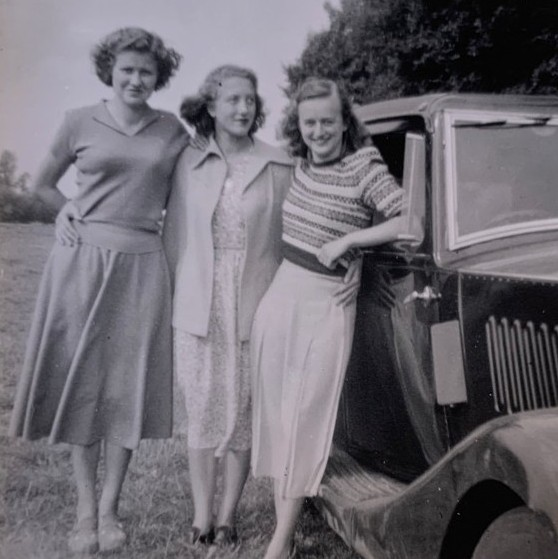
\includegraphics[width=1\textwidth]{boek_Tine_Blom.docx.tmp/word/media/image29.jpg}

Ik had \'{e}\'{e}n dag in de week vrij. Dan ging ik meestal op stap. Naar Londen Bijvoorbeeld. Met de trein. Ik ben \'{e}\'{e}n keer zelfs helemaal naar de zuidkust gegaan! Dat was prachtig. 

In mijn tijd in Walton on Thames heb ik een paar andere Nederlandse meisjes ontmoet. Daar was het wel leuk mee, alleen thuis zouden het niet mijn vriendinnen geweest zijn. 

Er waren geen leuke jongens. Daar had ik eigenlijk ook helemaal geen behoefte aan. En tja, dat is zo lastig een lange afstandsrelatie met een man uit Engeland. Er waren in de buurt een keer een stel Hollandse voetballers op bezoek. Toen kreeg ik een uitnodiging voor een ‘gezellige avond’. Daar had ik helemaal geen zin in! Haha. Ik ben wel ooit een leuke Amerikaanse jongen op de fiets tegengekomen. Maar dat was uiteindelijk toch ook niks.

Het gezin was heel prettig. Het waren beschaafde en bescheiden mensen. Ik hoorde van de andere Nederlandse meisjes die daar ook werkten dat dat soms wel anders was. Dan moesten ze een bejaarde vrouw verzorgen bijvoorbeeld, en ja dan ontmoette je verder ook niemand! 

Ik moest in het huishouden ook koken. Uitdaging was dat ik daar ineens Engels moest koken. Op een dag kwam de heer des huizes naar beneden om een compliment te geven over het uitstekende eten. Nou dat was heel wat! 

Opvallend vond ik dat wanneer ‘de heer des huizes’ thuiskwam van werk hij steevast mopperde over dat de mensen zo weinig met elkaar praatten in de trein. Dan zaten er elke dag dezelfde mensen in de trein, maar niemand deed zijn mond open! Dat vond hij verschrikkelijk. Maar zo zijn ze. De Engelsen. 

Het leukste vond ik dat ik opgegeven moment in het Engels droomde. Dat kwam omdat je het natuurlijk de hele dag sprak, en ja dan droomde ik ineens in het Engels! 

Na een tijdje in Engeland te hebben gewoond was mijn Engels dan ook ‘’ontzettend goed’’ 

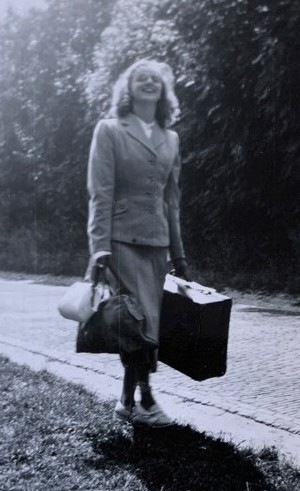
\includegraphics[width=1\textwidth]{boek_Tine_Blom.docx.tmp/word/media/image30.jpg}Het grootste compliment wat ik kreeg kwam van een dame van de winkel waar ik een jasje aan het passen was. Ik zei tegen de mevrouw die me aan het helpen was: ‘dit jasje vind ik niet zo leuk’. Waarop de dame van de winkel antwoorde: ‘’Oh, die lijkt natuurlijk een beetje op wat u op de kostschool gedragen heeft!’’ En ik heb natuurlijk nooit op de kostschool in Engeland gezeten. 

Ik heb het ontzettend naar mijn zin gehad. Maar Nederland was mijn thuis. Mijn ouders en familie waren er nog. En ja daar wilde ik natuurlijk wel een beetje bij in de buurt zijn. Ik wilde eigenlijk maar een jaar blijven. Maar op een dag kwam de vrouw des huizes naar me toe en zei: ‘’Och Tine, zou je alsjeblieft nog even willen blijven? Ik ben namelijk weer in verwachting’’ En toen ben ik nog een half jaartje langer gebleven. En dat vond ik wel genoeg. Ik had mijn doel bereikt. 

Na terugkomst uit Londen ben ik eigenlijk gelijk aan het werk gegaan. En ben ik terecht gekomen in Huis ter heide. 

\textit{Op vakantie naar Holland }



  Wil je nog meer weten over Londen?? Nah, nou is het klaar hoor! Haha (Einde interview) 

\chapter{\label{ref-007}Werken in Amsterdam}

\textit{Op het Wilhelmina Gasthuis }



 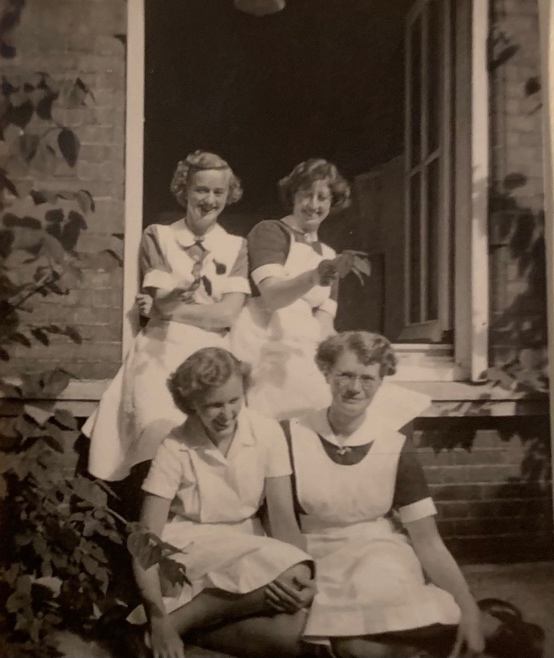
\includegraphics[width=1\textwidth]{boek_Tine_Blom.docx.tmp/word/media/image31.jpeg}Na Engeland heb ik in Amsterdam gewerkt; intern in het Wilhelmina gasthuis. Ik zat in die periode veel in het Vondelpark, ik vond dit een leuke tijd maar ik moet er nu niet meer aan denken om in Amsterdam te wonen. In het Wilhelmina gasthuis werkte ik als huishoudkundige, ik gaf leiding aan de meisjes die daar werkten in de huishouding. Ze noemden me dan Juf, zo hoorde dat. Ik dacht toen; dit werk wil ik niet blijven doen tot aan mijn pensioen.

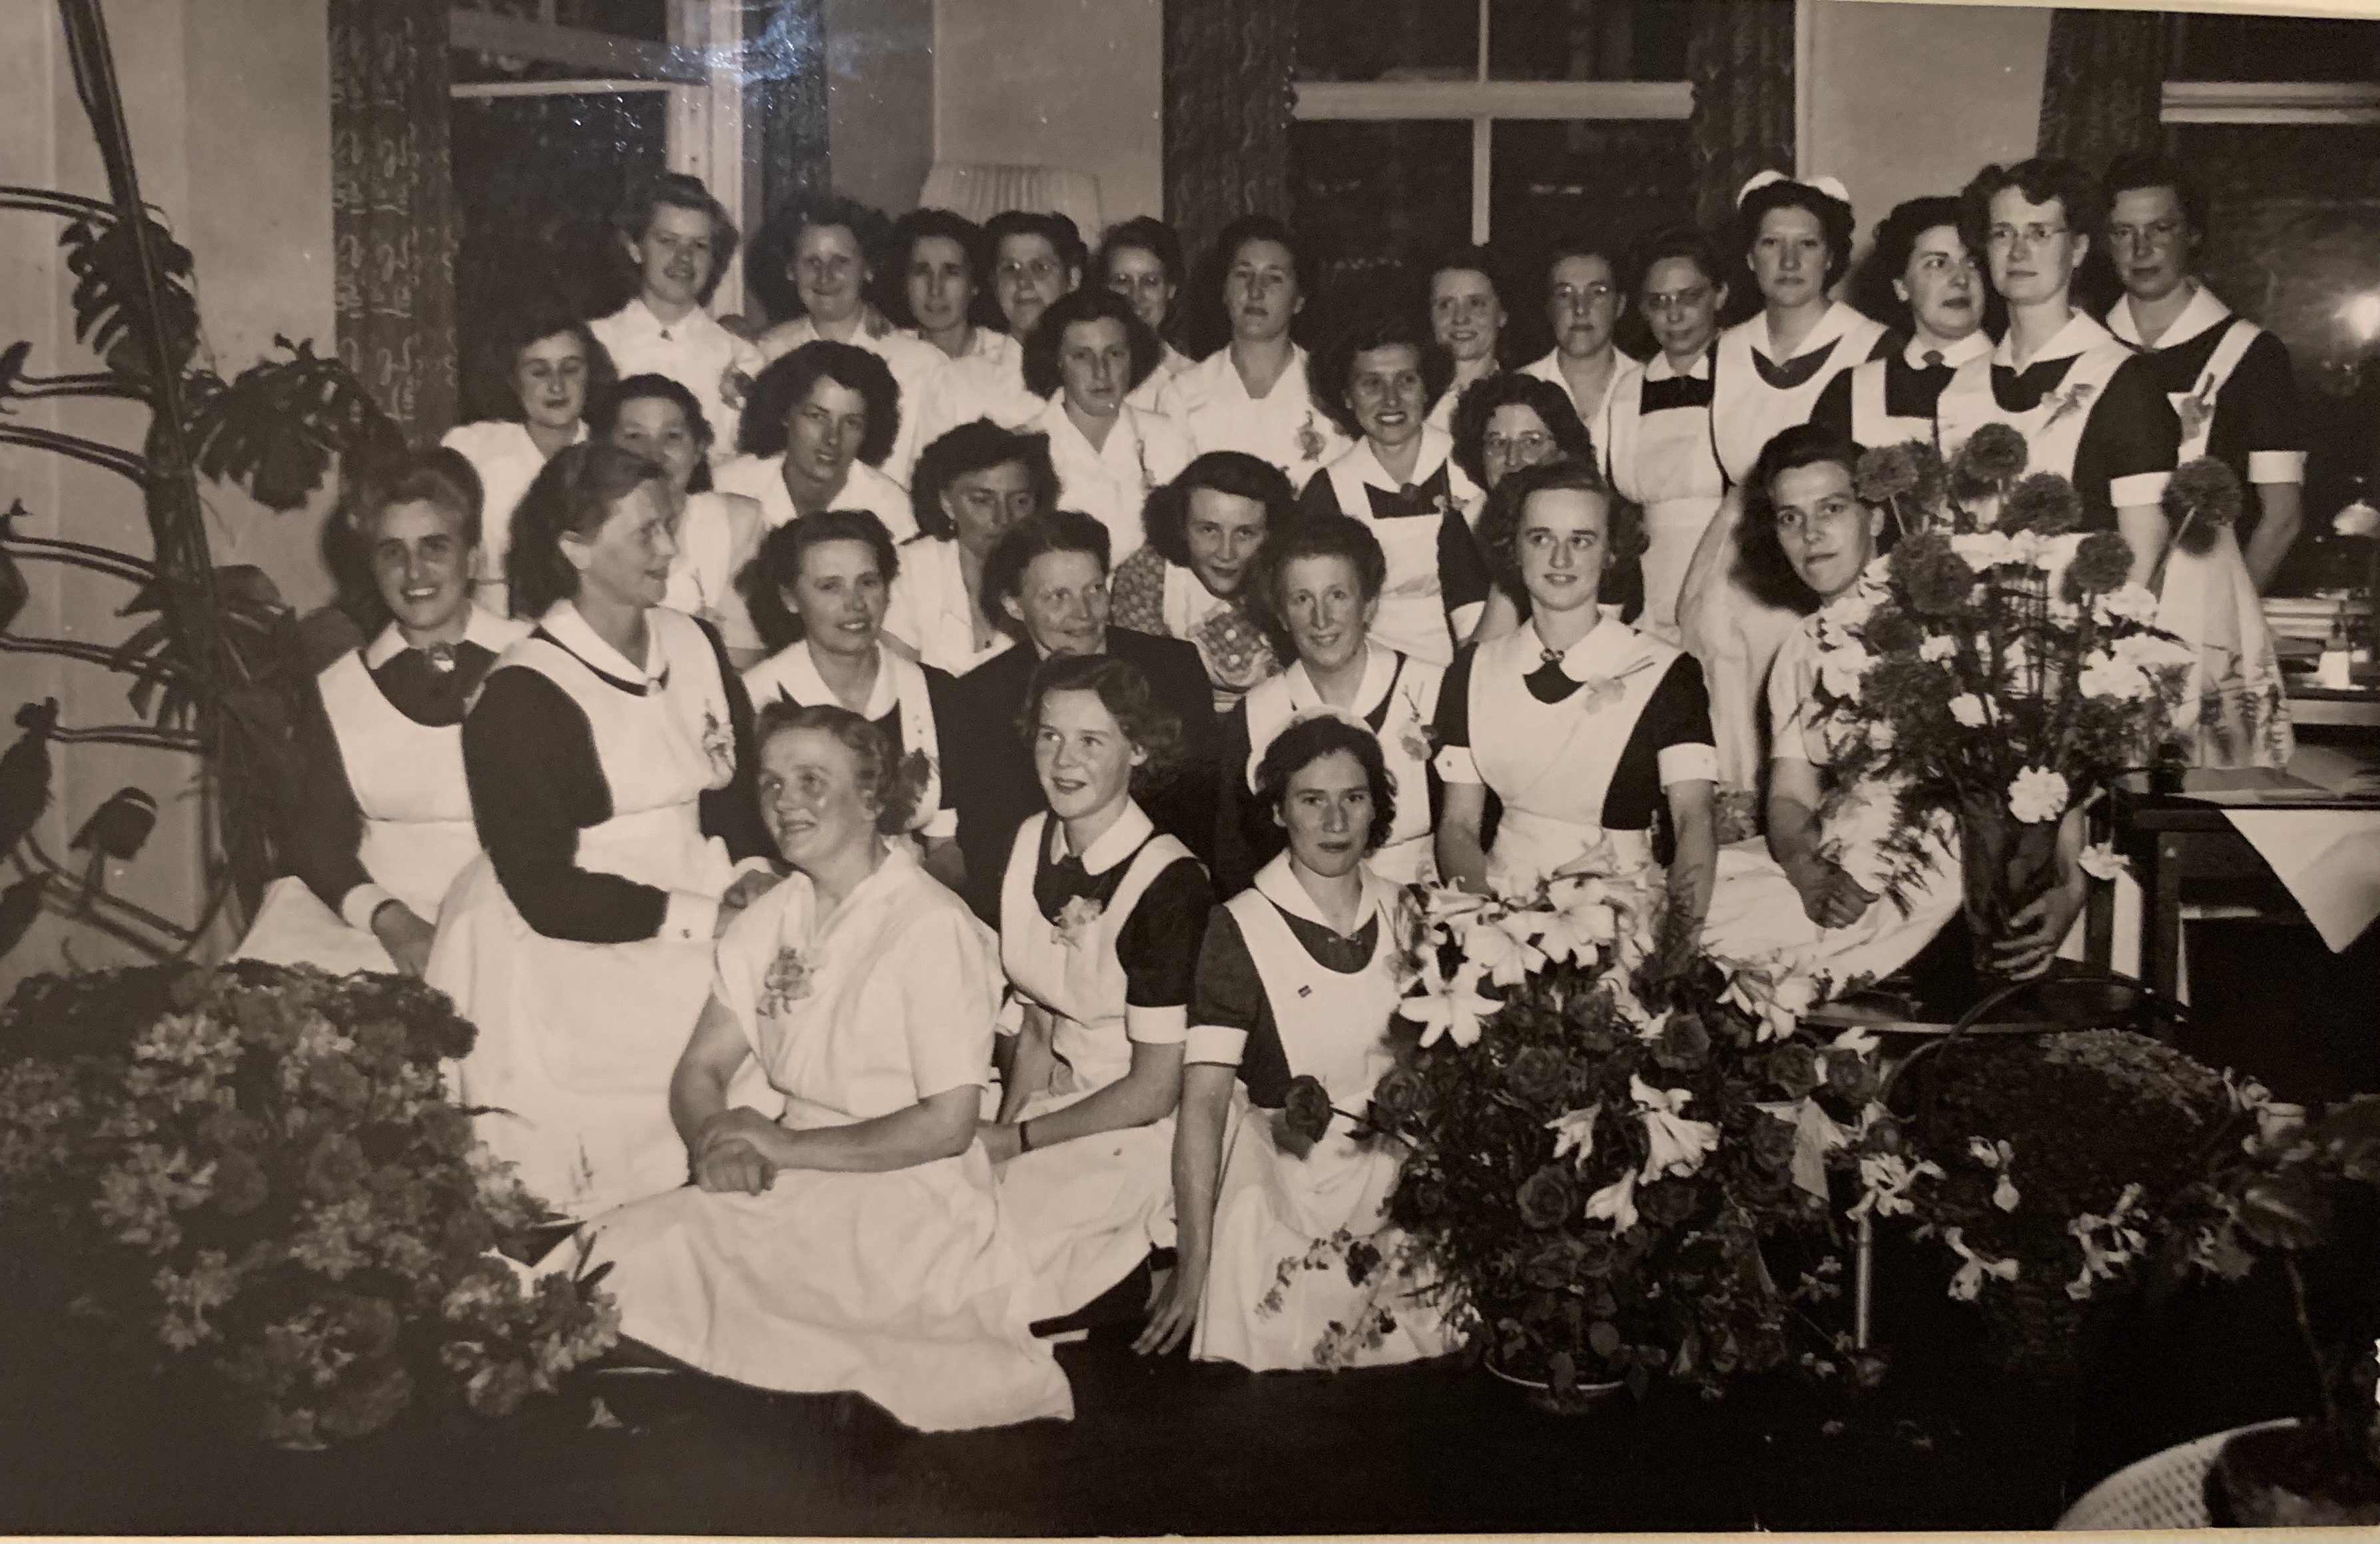
\includegraphics[width=1\textwidth]{boek_Tine_Blom.docx.tmp/word/media/image32.jpg}

\chapter{\label{ref-008}Werken bij de Kinderbescherming}

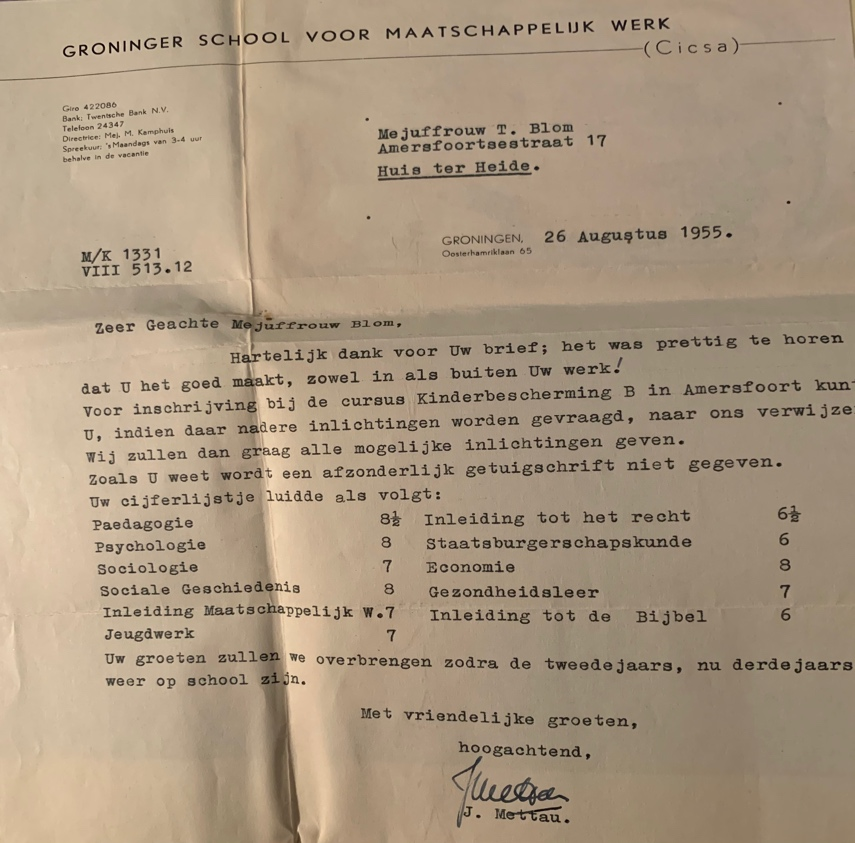
\includegraphics[width=1\textwidth]{boek_Tine_Blom.docx.tmp/word/media/image33.jpeg}

Daarna ben ik begonnen bij de Kinderbescherming in huis ter Wege (in het dorp Huis ter Heide). Eerst had ik hier de leiding in de keuken (koken voor 50 mensen) en daarna heb ik daar als jeugdleidster gewerkt. Intern heb ik hier een opleiding voor gedaan zodat ik met deze jeugd kon werken. In Groningen kreeg ik dan les, dit moest in mijn vrije tijd. Hier kreeg ik ook lessen in de psychologie, dat vond ik heel interessant. 

Totdat ik ging trouwen heb ik hier gewerkt, ongeveer van mijn 22\textsuperscript{e} tot mijn 28/29\textsuperscript{e}. In Huis ter Heide had je \'{e}\'{e}n jeugdleidster per afdeling van 12 kinderen, en je zat intern maar je had wel je eigen kamer.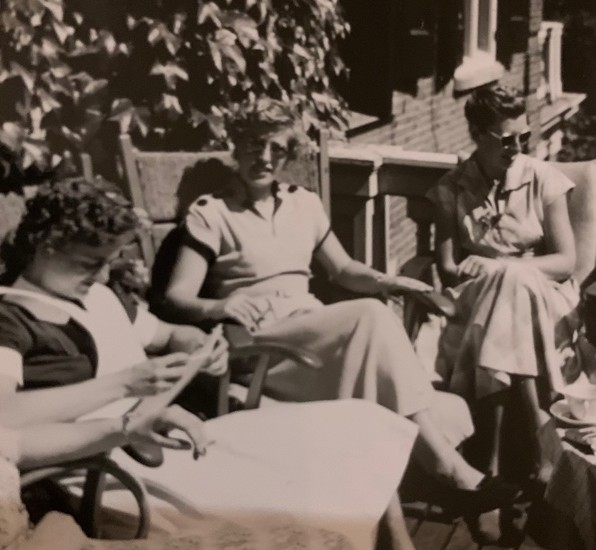
\includegraphics[width=1\textwidth]{boek_Tine_Blom.docx.tmp/word/media/image34.jpeg}\textit{de staf van Ter Wege drinkt koffie }



 

Ik begon daar met werken in de keuken, een paar meisjes hielpen mij dan. Daarna kreeg ik steeds meer taken, waaronder kookles geven het maken van de planning en het rooster. Ik ben ook nog een periode waarnemend directrice geweest. Ik vond het leuk werk, vooral het werken met kinderen. 

Deze kinderen werden vrijwillig geplaatst door het maatschappelijk werk of de school en ze knapten vaak flink op van hun verblijf bij ons. Als de kinderen binnenkwamen moesten ze vaak huilen, ik zei dan; als jullie over 3 maanden vertrekken dan moeten jullie weer huilen en dat was ook altijd zo. De kinderen waren 10 tot 12 jaar. Er was eens een meisje uit Egmond aan zee wat na haar verblijf langs kwam op bezoek, dit vonden we heel erg leuk. 

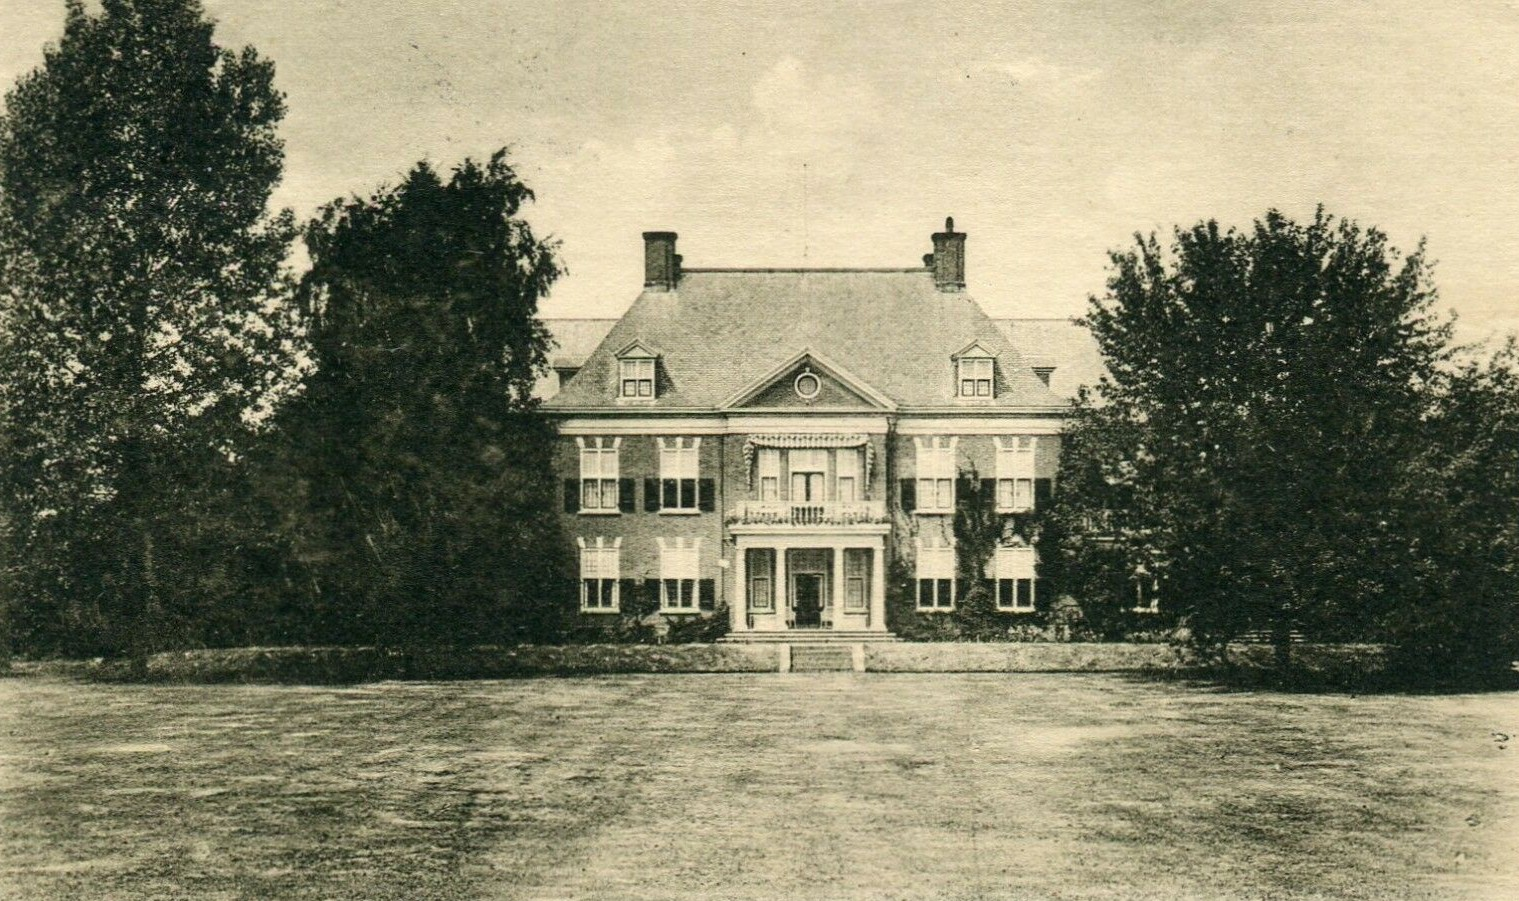
\includegraphics[width=1\textwidth]{boek_Tine_Blom.docx.tmp/word/media/image35.jpeg}\newline


\chapter{\label{ref-009}De liefde}

\textit{first love }



 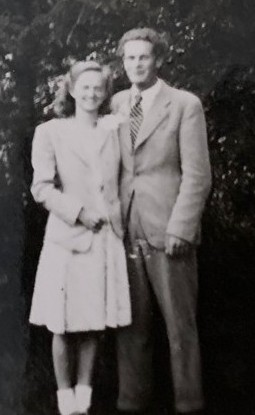
\includegraphics[width=1\textwidth]{boek_Tine_Blom.docx.tmp/word/media/image36.jpg}Voor Joop heb ik een ander vriendje gehad me wie ik wel serieus was. Hij woonde in Warmenhuizen maar dat heb ik na een poosje uitgemaakt. Ik wilde nog van alles, reizen en werken en hij wilde al trouwen en settelen en daar was ik nog niet aan toe. En na hem kwam Joop. 

Hoe Joop en ik elkaar ontmoet hebben? Dat is wel een leuk verhaal. Hij was thuis met studieverlof voor zijn tweede rang. Hij had eerder een keer een reis met mijn broer gemaakt en toen kwamen ze tot de ontdekking dat ze beiden een zus hadden. Hij had toen eens een foto van mij gezien en vond me er kennelijk wel leuk uitzien.

En toen heeft hij mee een kaart geschreven, die hij naar Huis Ter Wege stuurde waar ik werkte. Hij schreef dat hij graag een afspraak wilde maken, en dat vond ik wel leuk! Ik vond het niet heel gek of eng want ik wist dat Kees hem wel kende. Dus het was niet zomaar echt helemaal een onbekende voor me. En ik geloof dat ik hem ook ooit eens gezien heb, op een feest van Kees. 

\textit{Joop met zijn ouders en broer en zussen }



 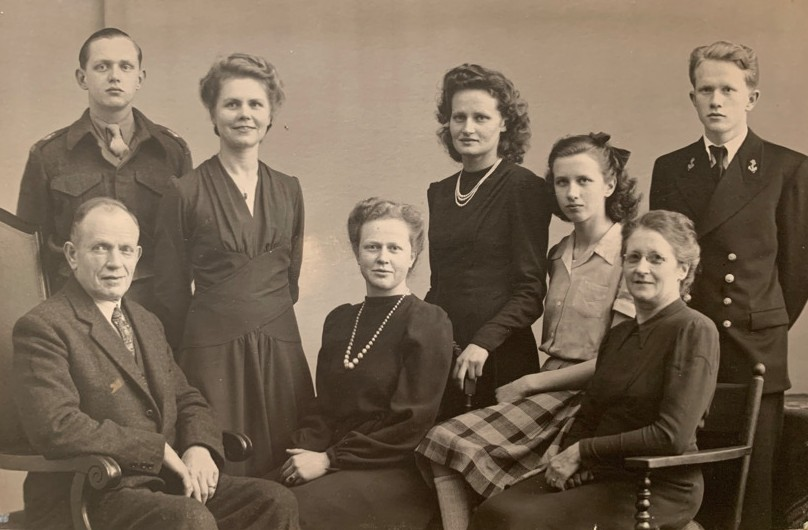
\includegraphics[width=1\textwidth]{boek_Tine_Blom.docx.tmp/word/media/image37.jpg}Hij was op zoek, dat was wel duidelijk. Dus we hebben een afspraak gemaakt in Utrecht. Toen ik hem zag vond ik hem er wel gelijk leuk uitzien, we zijn ergens gaan zitten koffiedrinken en hebben uren gepraat. We hebben eigenlijk maar heel weinig gewandeld kan ik me herinneren omdat we zoveel aan het praten waren. Hij bracht me met de taxi terug naar huis, terwijl ik gewoon met de trein naar Utrecht was gekomen. Het was al avond toen ik terugging dus toen vond hij het beter als ik met de taxi ging. Dat vond ik wel netjes van hem. Hij is in de taxi blijven zitten en niet eens mee naar binnen komen omdat het al laat was, maar daarna hebben we veel meer afspraakjes gehad. 

Ik viel op hem omdat hij leuk kon praten, hij kon leuk dingen vertellen en hij was hartstikke lief voor me. Het is heel anders als je een vriend hebt die vaart natuurlijk, dan was het echt feest als hij weer even verlof had. Dan gingen we leuke dingen doen. Dan zei ik wel dat we niet altijd op stap hoefden te gaan, maar hij zei dat dat juist wel moest omdat daar niks meer van zou komen als we kinderen hadden. We moesten er nog maar van genieten, zei hij. We deden niets bijzonders, want we vonden het eigenlijk gewoon al geweldig om bij elkaar te kunnen zijn. Maar maakten gewoon uitstapjes. Ik mocht hem alleen niet meenemen naar de bioscoop, want daar hield hij niet van. Maar we gingen wel naar de schouwburg, in Amsterdam waar we ook een keertje in een hotel hebben geslapen. Dat was echt heel leuk.

We kenden elkaar eigenlijk nog helemaal niet zo lang toen en toen moest hij een jaar naar Zuid-Afrika. Dat vond ik erg spannend en ook wel moeilijk, maar door een geluk bij een ongeluk kwam hij al veel eerder naar huis omdat hij malaria kreeg. Daar werd hij erg ziek van en toen wilde ze vanuit de maatschappij dat hij naar Nederland kwam tot hij weer beter was.

Als hij weg was schreven we elkaar. We hebben wat afgeschreven toen hij voer, dat was het enige communicatiemiddel dat er was. Tegenwoordig kun je een stuk gemakkelijker communiceren, maar als hij op reis was, was hij ook echt w\'{e}g. En dus konden we alleen in contact blijven door elkaar brieven te schrijven. Hij heeft weleens gebeld, maar dat wilde ik niet meer want dan hoorde ik zijn stem wel maar was hij er niet en dan miste ik hem een stuk meer dan wanneer we gewoon alleen maar schreven. Dus toen hebben we afgesproken dat we niet meer gingen bellen. 

Wel heeft hij ooit eens iets bijzonders gedaan, en dat is flessenpost sturen. Hij had de fles ergens in Itali\"{e} in de buurt van vissersschepen in het water gegooid, en hij had gezien dat die vissers de fles uit het water hadden gehaald. Hij had er wat geld in gedaan zodat de vissers de brief ook zouden posten en zo is hij bij mij aangekomen. Dat was wel heel bijzonder, dat was een brief op een onverwachts moment. Dat was dus een hele leuke verrassing kan ik me nog herinneren.

Soms duurde het wel een week voor ik een brief ontving als hij vertrok vanuit Rotterdam. En ik stuurde dan een brief terug, want ik kreeg een lijst met alle havens die hij aandeed onderweg. We hebben heel wat afgeschreven, maar ik heb ze niet bewaard. Ik vind dat het iets tussen ons twee\"{e}n is. Achteraf had ik ze misschien wel moeten bewaren, maar ik heb ze allemaal verbrand omdat het me heel naar lijkt dat anderen ze zouden kunnen lezen. Ik liep eens met Jacqueline langs een tweedehands winkel en in de etalage lagen oude brieven en dat deed me beseffen dat ik niet zou willen dat mijn brieven zo zouden belanden als ik er niet meer ben, vandaar.

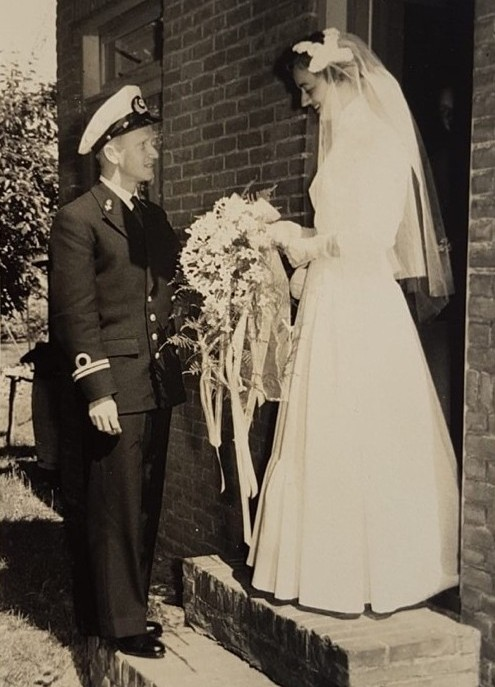
\includegraphics[width=1\textwidth]{boek_Tine_Blom.docx.tmp/word/media/image38.jpeg}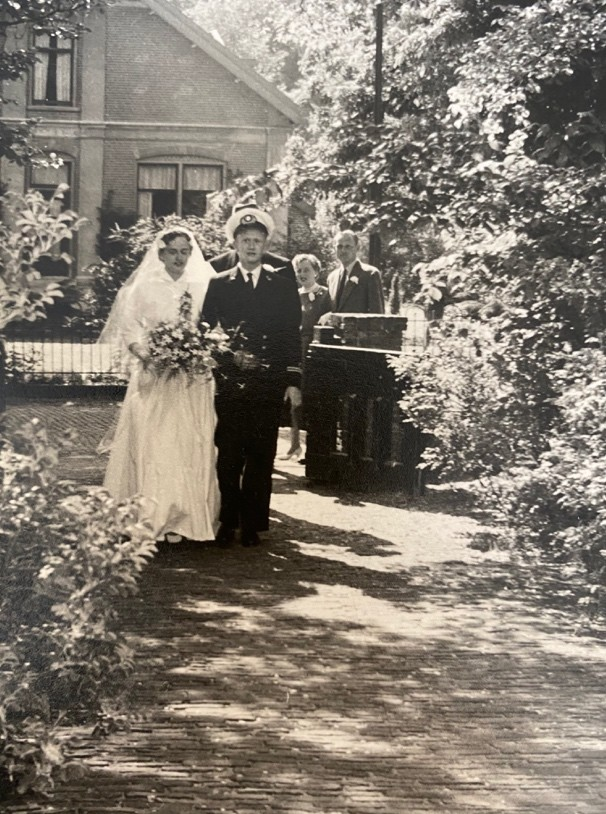
\includegraphics[width=1\textwidth]{boek_Tine_Blom.docx.tmp/word/media/image39.jpeg}En toen zijn we getrouwd. Maar van het aanzoek kan ik me eigenlijk nog maar weinig herinneren. We waren hartstikke verliefd maar hij ging niet op zijn knie\"{e}n met een ring, ik weet niet eens meer hoe dat ging. Het was wel leuk hoor! Het liep gewoon natuurlijk zo omdat we elkaar leuk vonden. Ik had het ook niet gewild dat hij op zijn knie\"{e}n ging, dat had ik verschrikkelijk gevonden. Ik vind dat belachelijk, dat een man op zijn knie\"{e}n moet gaan, je doet het toch samen? Ik had hem z\'{o} mijn zijn kraag gepakt en gezegd dat hij gauw weer moest gaan staan!

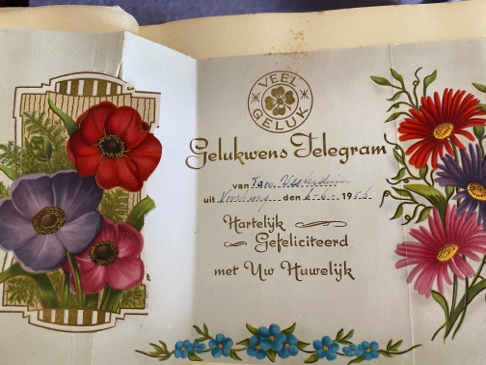
\includegraphics[width=1\textwidth]{boek_Tine_Blom.docx.tmp/word/media/image40.jpeg}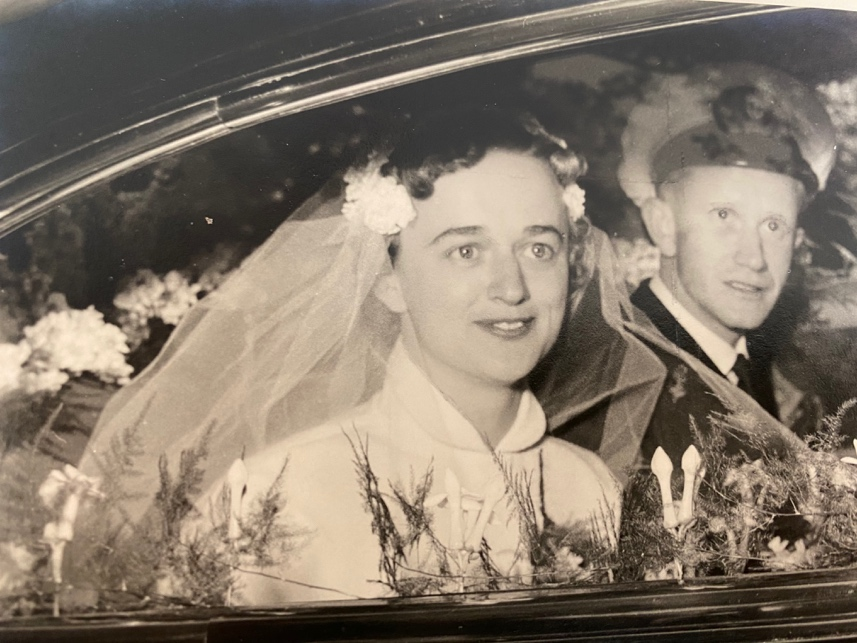
\includegraphics[width=1\textwidth]{boek_Tine_Blom.docx.tmp/word/media/image41.jpeg}We zijn getrouwd in 1956, in Schoorl. De trouwjurk heb ik met mijn moeder in de Bijenkorf in Amsterdam gekocht, Het duurde niet heel lang tot ik hem had gevonden, ik vond hem gelijk die middag wel. Over de trouwdag zelf weet ik niet heel veel meer. Ik denk dat ik wel zenuwachtig was maar dat weet ik echt niet meer. De hele familie van mij en Joop kwam, en het was wel een hele mooie dag. Hij droeg zijn uniform, en zag er heel mooi uit. Het scheelde ook in kosten, want zo hoefde hij niet nog een duur pak te kopen. Na het huwelijk hadden we een diner in een restaurant en dat was heel leuk en gezellig in kleine setting.

\textit{op huwelijksreis in Chamonix }



 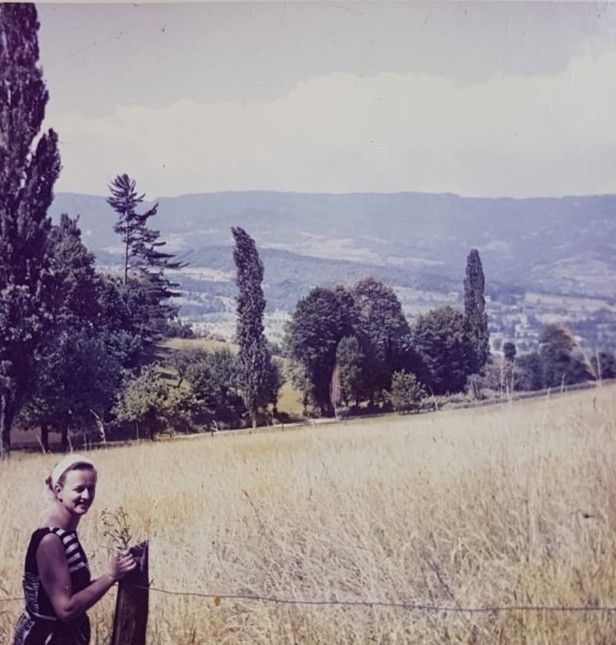
\includegraphics[width=1\textwidth]{boek_Tine_Blom.docx.tmp/word/media/image42.jpeg}Na ons trouwen zijn we op huwelijksreis geweest in Frankrijk.

We wilden niet direct aan kinderen beginnen, maar ik was 29 dus dat vond ik wel een mooie leeftijd om moeder te worden. Maar toen de kinderen er net waren moest Joop alweer varen. Dit was natuurlijk niet fijn, maar ik wist dat het zo zou lopen en was het al gewend dat hij langere periodes wegging. Dan stonden we te wuiven en ging hij weer. Ik was altijd wel verdrietig en zou hem erg missen, maar ik moest niet huilen als hij wegging. Dat wilde ik hem niet aandoen. 

En toen veel later zijn we naar Valthe verhuisd. Toen we in Valthe zijn gaan wonen voer hij ook nog, maar toen werd hij ziek. Hij kreeg last van zijn keel, ik herinner me dat niet allemaal meer hoor. We wisten al wel snel dat het niet goed was. Als ik terugkijk op ons huwelijk was het wel fijn, maar hij heeft natuurlijk wel veel gevaren en dat is niet leuk. Maar als hij thuis was was het wel heel fijn. Dan was het echt feest en genoot ik heel erg van het samenzijn.

En de mooiste herinnering die ik heb aan hem en ons? Dat is toch dat ik aan de kade stond en dat het schip weer aankwam waarop hij zat, nadat hij een jaar gevaren had. Dat gevoel was zo fijn, dat kan ik me nog precies voor de geest halen.''

\chapter{\label{ref-010}Hilversum, Den Haag, Dordrecht: kinderen}

Nadat ik getrouwd was moest ik dat doorgeven aan het kantoor van de Kinderbescherming in Den Haag en kreeg ik dus (!) mijn ontslag. Maar ik mocht toch wel doorwerken en werd voortaan gedetacheerd als er ergens te weinig mensen waren. Ik wilde wel graag doorwerken want Joop voer dus ik was best veel alleen.

Ik vond het leuk om te trouwen maar ik kon het niet uitstaan dat ik stoppen moest met werken. Ik vond het verschrikkelijk dat ik mijn eigen geld niet meer kon verdienen toen de kinderen werden geboren, ik vond dat ik zelf voor een inkomen moest zorgen. Maar dat kon niet, het ging anders. Ik was 29 jaar toen ik ging trouwen.\newline
 

Toen de kinderen groot waren heb ik nog wel eens overwogen om weer aan het werk te gaan. Mij is toen verteld dat ik het waarschijnlijk niet leuk meer zou vinden omdat het gedrag van de kinderen heftiger was dan in de tijd dat ik nog werkte, ik heb toen besloten om het niet te doen.

We hebben eerst ingewoond in Hilversum bij de moeder van een collega, mevrouw IJma. We hadden een eigen etage met een flinke kamer boven met een slaapkamer. Koken was een beetje primitief in een soort werkkast met een elektrisch pitje. Het was best wel leuk. Joop ging natuurlijk weer varen; nog wel korte reisjes van 2 tot 3 maanden. 

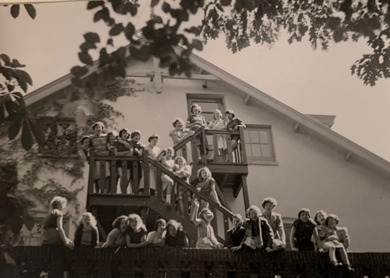
\includegraphics[width=1\textwidth]{boek_Tine_Blom.docx.tmp/word/media/image43.jpg}\textit{Gedetacheerd in Den Dolder }



 Ik werkte onder andere bij een instelling voor kinderbescherming in Den Dolder en Hilversum voor iets oudere kinderen (14-17). Daar werkte ik als waarnemend directrice. Ik moest de werkzaamheden van iedereen inplannen en viel in op de groepen als het nodig was. Ik werd gedetacheerd naar diverse instellingen.

Na een tijdje gingen we verhuizen naar Den Haag. Via de zus van Joop konden we in het huis van hun buren terecht. Daar konden we een deel van onderhuren. Het was een ouder echtpaar en ze waren er vaak niet. En gelukkig waren ze reuze makkelijk. Zij hadden daar de voorkamer en wij de achterkamer met een klein slaapkamertje en een balkon. De woningnood was toen, zo vlak na de oorlog, nog erg groot. 

Toen we net getrouwd waren ging Joop weg op een ontzettende lange reis. Toen we net verloofd waren ging hij een jaar weg, maar toen werkte ik nog, dus was het gemis minder. Op een gegeven moment kwam er een beter ritme met kortere reizen. Vooral toen hij naar Zuid-Afrika ging, want dat waren zes weken. Maar ja, dat wilde iedereen wel natuurlijk, dus dat moesten ze een beetje verdelen. Nou ja, het gebeurt en de \'{e}\'{e}n kan er tegen en de ander niet. Als je niet z\'{o} bij moeder vandaan komt en dan trouwt met iemand die constant weg is gaat het beter. Als je je eigen werk hebt.

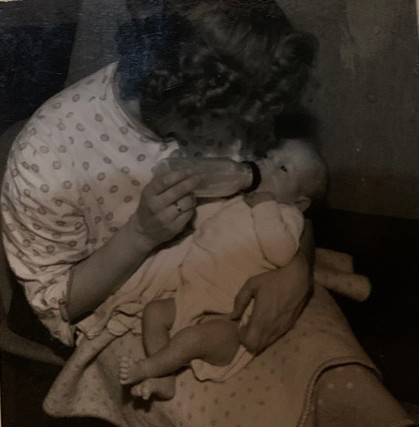
\includegraphics[width=1\textwidth]{boek_Tine_Blom.docx.tmp/word/media/image44.jpg}Ik raakte in Den Haag in verwachting en stopte met werken. Jacqueline is op 4 februari 1958 in het ziekenhuis geboren. Joop was net van een kustreis terug. Hij kwam thuis van een lange reis en moest daarna nog een kustreis en dat ging allemaal n\'{e}t! Jacqueline is in de Oranjekliniek in Den Haag geboren, want we woonden in. We hadden geen ruimte om thuis te bevallen.

Joop studeerde toen voor zijn tweede rang; hij moest daarvoor naar school in Amsterdam. Dat kwam wel even mooi uit. Ik moest wel wennen toen hij daarna weer weg ging en ik alles alleen moest doen.

We hebben dus nog een jaar ondergehuurd met een baby. Het was vooral gezellig met m’n schoonzus en zwager als buren. 

En we zaten vlak bij het Haagse bos. Ik ging vaak wandelen met Han, mijn schoonzus en onze baby’s. Ik had het er best naar mijn zin!

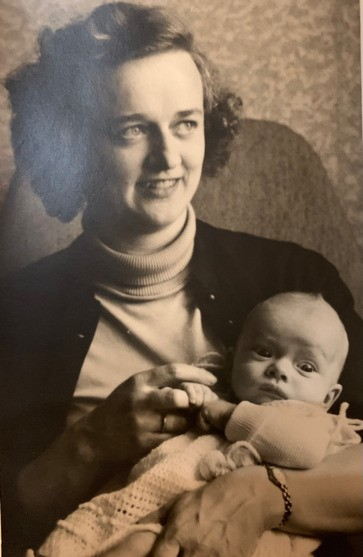
\includegraphics[width=1\textwidth]{boek_Tine_Blom.docx.tmp/word/media/image45.jpg}

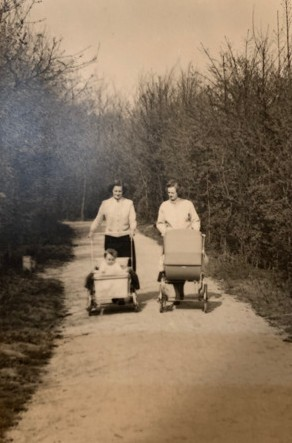
\includegraphics[width=1\textwidth]{boek_Tine_Blom.docx.tmp/word/media/image46.jpg}  

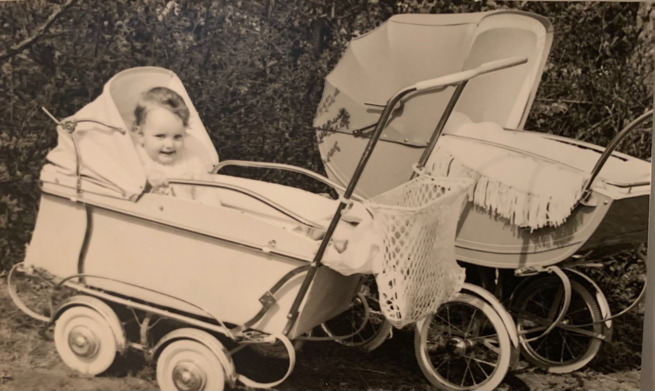
\includegraphics[width=1\textwidth]{boek_Tine_Blom.docx.tmp/word/media/image47.jpg}

De maatschappij waar Joop werkte, de VNS, liet vervolgens in Dordrecht een appartementengebouw neerzetten voor zeevarenden. Daar kregen wij eindelijk ons eerste eigen huis! 

De hunkerbunker noemden de mannen dat gebouw. Want ja met al die vrouwen van zeevarenden daar...

Ik kon er wel tegen; ik zocht wat anders om me mee bezig te houden. Ik was gelukkig al jaren zelfstandig. Maar er waren ook vrouwen die er echt niet tegen konden. Dat was het laatste wat ik wou, dat mijn man met zijn werk moest stoppen omdat ik niet op mijn eigen benen zou kunnen staan. Maar ik had het af en toe ook wel moeilijk.

In de flat kreeg ik een leuke vriendin, Jannie Punt. Wij hebben ons hele leven contact gehouden. Maar nu we zo heel oud zijn wordt dat wat lastiger. Het waren verder beste mensen, maar daar ging ik niet mee om. Jannie Punt was degene waar ik het meeste contact mee had.

\textit{Yvonne }



 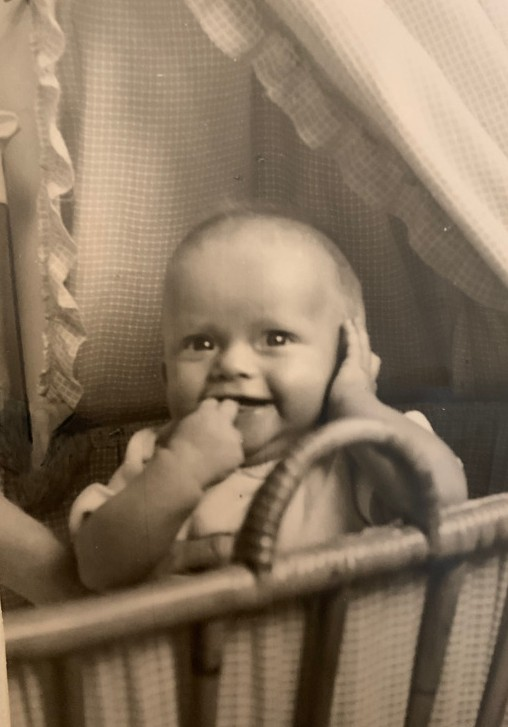
\includegraphics[width=1\textwidth]{boek_Tine_Blom.docx.tmp/word/media/image48.jpg}

In Dordrecht is Yvonne geboren, op 20 april 1959, ruim een jaar na Jacqueline.

Een hele aardige dokter had ik toen. Hij was ook gewoon zorgzaam, zo van ‘die man zit op zee...’.

Joop was toen ook een periode wat langer thuis voor z’n eerste rang te halen; hij moest in Scheveningen naar de zeevaartschool. Dat was wel een hele leuke en gezellige periode! Hij had ook een vak in het Engels en dat deden we dan samen. 

De bevalling was ’s nachts al begonnen en ik dacht: Ik ga die dokter nog niet bellen, maar tegen 7 uur vond ik het wel tijd worden. Hij kwam ook snel en Yvonne werd thuis geboren. 

En het was hartstikke gezellig hoor, het thuis bevallen. Als het allemaal goed gaat, vind ik dat thuis veel leuker. En het waren geen zware bevallingen. Ik zei wel eens: ``Wat dat betreft kan ik er wel 12 op de wereld zetten.'' Jacqueline was net bij Jannie Punt gebracht en de melkboer kwam aan de deur en zei tegen Joop: ik hoor volgens mij al een baby huilen. Kortom een zeer snelle geboorte.

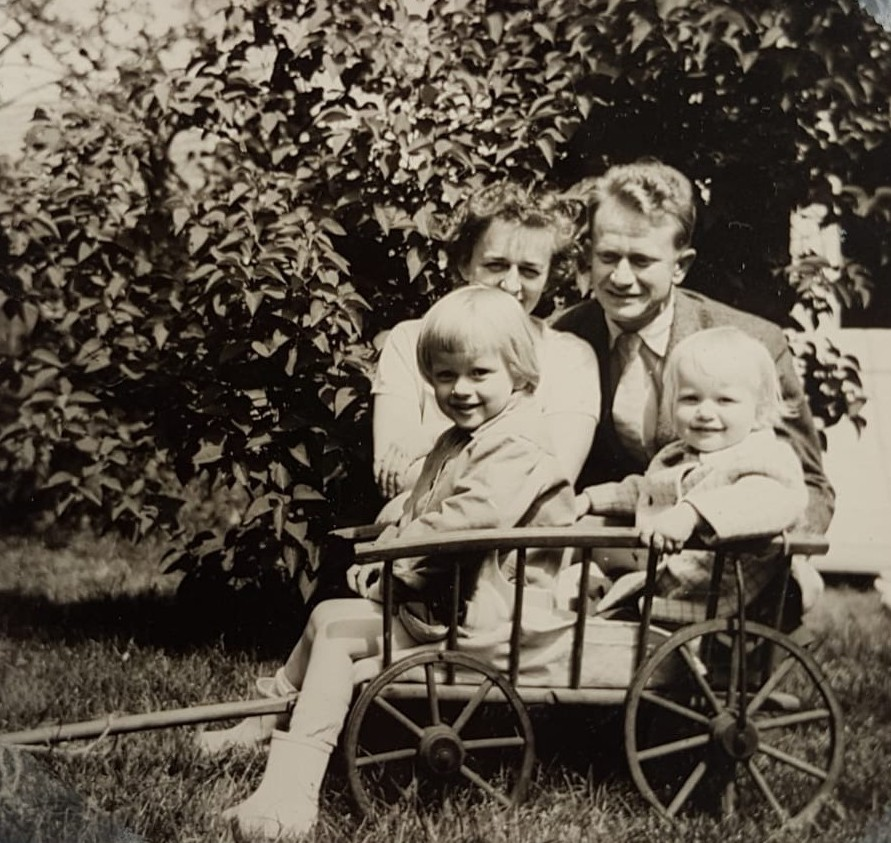
\includegraphics[width=1\textwidth]{boek_Tine_Blom.docx.tmp/word/media/image49.jpg}Ik kreeg Jacqueline en Yvonne snel achter elkaar. Toen wist ik wat ik moest doen. Ik vond het voor de kinderen leuk dat ze zo weinig scheelden.

\chapter{\label{ref-011}Doorn}

Joop kwam een keer thuis van een reis en hij zei: ``We gaan een huis kopen! We kunnen wel blijven sparen, maar we nemen gewoon een hypotheek.'' Dan draag je regelmatig geld af en omdat hij een goeie baan had kon dat best. Toen zijn we in Doorn terecht gekomen, want ik dacht: ``Ik ga niet in Schoorl wonen''. Dat leek me niet goed. Zo zaten we centraal, want hij moest soms ook bijwerken en dan moest hij naar Rotterdam, of Amsterdam en dat was te doen.

Het was wel fantastisch natuurlijk om een eigen huis te hebben. Het huis had een ander laten bouwen, maar die ging er uiteindelijk niet in. 

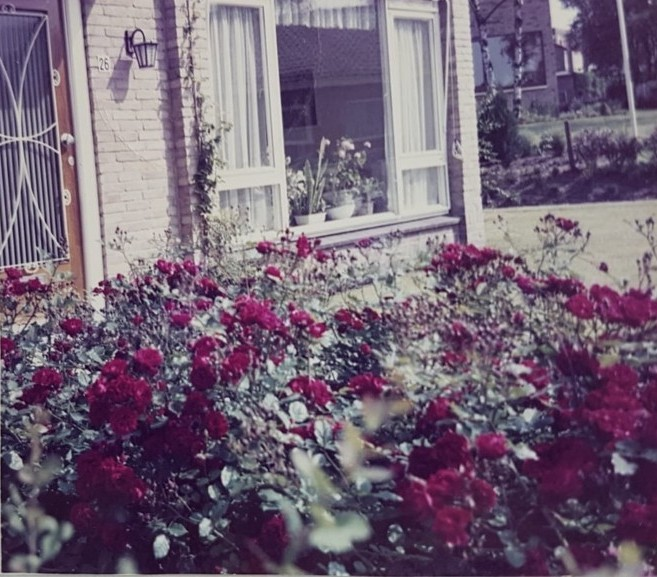
\includegraphics[width=1\textwidth]{boek_Tine_Blom.docx.tmp/word/media/image50.jpeg}Het was fijn aan de rand van het bos. Er hingen ook wel eekhoorntjes aan de pinda’s. Ik was wel blij dat we dat huis hadden, dat we daar gingen wonen. Want een appartement was ik niet gewend natuurlijk. Ik miste een tuin.

Al gauw kwam ‘tante’ Betty er wonen met haar man en ook de familie van Putten. Die gingen eerder al weer weg. Daar zijn we ook nog geweest, op de Veluwe. (dat weet dochter Yvonne nog goed..zij speelde zo graag met Tink). Tegenover woonde Toek Beekman (tante Toekie) met haar man. Ik kon wel met haar omgaan. Ik moest wel om haar lachen, maar de kapiteins zeiden: ``Ik wil die vrouw niet meer aan boord hebben''. Als pappa de auto ging schoonmaken, was ze er ook ineens. Ze hing om andere mannen heen blijkbaar. Maar ik ben wel steeds gewoon met haar omgegaan.

\includegraphics[width=1\textwidth]{boek_Tine_Blom.docx.tmp/word/media/image51.jpg}Ja, we hebben daar altijd wel lekker gewoond, hoor. Om dat pleintje. Ik zie de kinderen nog die bult op fietsen. Eerst bracht ik ze maar later gingen ze zelf naar school natuurlijk.

Joop kwam een keer thuis en zei: ``Ik ga een auto kopen''. Zo is het gegaan. Ik zei: ``Een auto kopen? Moet ik dan de boodschappen met de a\'{u}to doen?! Wat een onzin!'' 

Ik heb rijlessen genomen en de instructeur maakte zich altijd erg druk als er iets verkeerd ging. Dat deed hij niet zo bij mij, maar ik was er wel op voorbereid. Zijn vrouw gaf ook les en als ik dan zag dat zij in de auto zat was ik wel opgelucht. De lessen begonnen in Zeist. En ik weet nog wel dat ik daar een keer op de bus stond te wachten en dacht ``Wat een drukte hier en oh, daar zit ik dan ook in!'' Dat is natuurlijk wel anders dan. Maar ik realiseerde me eerst niet dat je achterlichten had en dat ze die ook wel zagen. Ik was nog bang dat ze tegen me op reden! Het rijbewijs heb ik wel in \'{e}\'{e}n keer gehaald.~

De eerste auto was Urania, een Fiat. Het bleek toch wel lekker te zijn om boodschappen te doen met de auto!

\includegraphics[width=1\textwidth]{boek_Tine_Blom.docx.tmp/word/media/image52.jpg}Ik was veel alleen met de kinderen maar ja, dat doe je gewoon en je moet niet vergeten, dat ik al langer zelfstandig was. Er waren wel vrouwen die het niet redden alleen. Dan moest de man een walbaan zoeken. Dat was het laatste wat ik Joop aan wilde doen, want hij vond het varen zo leuk. En ik kon er ook wel tegen.

Soms gingen we mee op kustreis. 

In de gang in Doorn hing een zwarte vaste telefoon. Joop belde dan wel eens, haast nooit. We hadden een keer afgesproken, toen waren de kinderen nog klein, dat hij een keer zou bellen. Toen was hij op reis. En wij zaten er helemaal klaar voor en dat is ook allemaal doorgegaan, maar we vonden het eigenlijk niks dat hij er niet bij was. Ik zei: ``Dat moet je maar niet meer doen''. Dan hoor je elkaar en dan voel je het gemis meer. En dat vonden jullie ook. We zeiden ooit tegen elkaar, hoe mooi het zou zijn als er een soort televisiefoon zou zijn, zodat je elkaar ook zou kunnen zien. Nou, dat is er wel gekomen (na een kerstviering via zoom vanwege de corona in 2020), maar een beetje te laat voor ons. Nou ja, je trouwt met iemand die vaart, dus zo is dat dan.

Op een gegeven moment liep ik in Doorn mijn vroegere vriendin Riekje tegen het lijf. Hoe ging dat? Ja, ik had al iemand zien lopen en dacht: ``Dat lijkt wel Riekje Bakker!'' Ik moet toch eens opletten. En toen fietste ik naar school om de kinderen op te halen en toen reed Riekje voor me! En ik riep: ``Ja, ik zie, het is haar!'' Ik kende haar van het Wilhelmina Gasthuis. Zij zat in de keukenafdeling en ik in de huishoudafdeling. Die keuken vond ik niks, met van die grote gamellen. Riekje was echt een lief mens. Jaren later woonden wij weer bij elkaar in de buurt in Drenthe. We zijn altijd vriendinnen gebleven. Jammer genoeg is ze nu overleden.

Jacqueline en Yvonne zijn opgegroeid in Doorn. Kleuterschool, Lagere school: Willem de Zwijgerschool en het Revius Lyceum. 

\includegraphics[width=1\textwidth]{boek_Tine_Blom.docx.tmp/word/media/image53.jpeg}In de vakanties troffen we het als Joop net met verlof was. Dan gingen we lang weg, naar Frankrijk, Spanje, Portugal of Joegoslavi\"{e}. Soms wilde ik dan wel weer naar huis.

We reden er 2 dagen over en ’s avonds dan stopten we en kampeerden we in het wild. Toen had ik net een verhaal gehoord dat mensen waren overvallen. Ik weet nog dat ik in de nacht een auto hoorde aankomen, maar het waren gewoon mensen die ook een plekje voor de nacht zochten. Die hadden ons zien staan en kwamen daar ook slapen.

\includegraphics[width=1\textwidth]{boek_Tine_Blom.docx.tmp/word/media/image54.jpg}Toen de kinderen 6 en 7 waren hebben we eerst een tent gehuurd en daarna een bungalowtent gekocht. De stokken waren gemerkt. In Luxemburg gingen we kamperen met zijn drie\"{e}n toen Joop niet meekon, en zo konden we de tent ook samen opzetten.

Ik vond dat er een hond bij moest. Bij mijn ouders was ook een hond, Blacky, toen wij als kinderen nog thuis waren en bij Joop thuis ook (ook al wandelden ze er niet zo veel mee).

Timba ging altijd mee wandelen op vakantie, Luxemburg, de Ardennen. En dan was hij z\'{o} moe van al het lopen. Dan legde ik wat vlees op zijn neus en hij was z\'{o} moe dat hij nergens meer op reageerde!

\includegraphics[width=1\textwidth]{boek_Tine_Blom.docx.tmp/word/media/image55.jpeg}Eerst hadden we in Doorn een schattig kacheltje wat we ook al in Dordrecht hadden, maar in Doorn was de kamer groter en kwam er een andere kachel, gestookt op kolen. Achter de garage was een kolenhok. Het was een makkelijke kachel, als hij \'{e}\'{e}n keer brandde deed hij het de hele dag. Maar het was wel ideaal toen we centrale verwarming kregen. En een open haard.

We hebben v\'{e}\'{e}l gewandeld in Doorn! Toen we eenmaal in het huis in Doorn woonden was dat eigenlijk de mooiste tijd. Het mooiste wonen ook. 

Het was een mooi plekje, zo bij het bos en een ruim huis. Het zorgen voor de vogels hoorde dar ook bij, dat deed mijn moeder ook en de buurvrouw Betty. Later werd de keuken nog verbouwd en kreeg Jacqueline een zolderkamer en Yvonne een dakterras aan haar kamer, die kleiner was met een opklapbed. Er was een barretje in de keuken en een open verbinding met de kamer. Veel gemakkelijker.

Toen de kinderen groter waren heb ik nog met ouderen gewerkt als vrijwilligster. Dat was wel leuk. Een betaalde baan was niet noodzakelijk en was druk. De jeugd is wel veranderd werd ik gewaarschuwd. Daarom heb ik nooit meer betaald werk gezocht.

In het eindexamenjaar heb ik heel wat zitten overhoren en toen gingen de kinderen tegelijk de deur uit. Jacqueline was een jaartje ouder (18) en ging studeren. Omdat Jacqueline ging, ging Yvonne ook uit huis. Zij was 17. Toen heb ik wel even moeten wennen. 

Met Joop ging het in die tijd ook niet altijd goed.

\chapter{\label{ref-012}\includegraphics[width=1\textwidth]{boek_Tine_Blom.docx.tmp/word/media/image56.jpeg}\includegraphics[width=1\textwidth]{boek_Tine_Blom.docx.tmp/word/media/image57.jpeg}Valthe en kleinkinderen}

Wat later ging Joop met vervroegd pensioen en verhuisden we naar Valthe, zodat er meer ruimte was: 1,5 ha grond. En een verbouwd boerderijtje. Er kwamen schapen en lammetjes, kippen en ganzen. En een moestuin. Dat was wel leuk. Drenthe is een prachtige provincie. Joop en ik reden een keer door Drenthe en eigenlijk kenden we Drenthe helemaal niet en toen zeiden we tegen elkaar: ``Wat is dit ook een mooie provincie!'' En toen besloten we dus dat we daar best konden gaan wonen. Nou, maar dan vind je natuurlijk niks, h\`{e}. En toen hebben we het uit handen gegeven aan een makelaar en die vond het huis aan de Vlintweg in Valthe. Want Joop had gezegd; ``Ik wil wel ruimte om me heen hebben''. Nou, zei \includegraphics[width=1\textwidth]{boek_Tine_Blom.docx.tmp/word/media/image58.jpeg}die makelaar, ruimte dat heb je dan wel.

Nou wat moet je daar dan als niet-landbouwer? Er kwam een heel kerstbomenbos en kippen en schapen en een hond. Ook lammetjes werden er geboren in de lente en dan soms moest er \'{e}\'{e}ntje met de fles worden grootgebracht, maar dat vond ik wel leuk, hoor! Zo ging ik op een dag naar het dorp om een zuigfles te kopen! Ja, dat heb ik ook allemaal gedaan...Er zijn ook nog foto’s van. 

 

Toen de kleinkinderen wat groter waren kwamen ze wel logeren in Valthe. Op zolder was de bedoeling, maar er was ook een logeerkamer beneden, waar ze vaak sliepen. Er was ruimte genoeg!

\includegraphics[width=1\textwidth]{boek_Tine_Blom.docx.tmp/word/media/image59.jpg}\includegraphics[width=1\textwidth]{boek_Tine_Blom.docx.tmp/word/media/image60.jpg}

Later werd Joop ziek en ik wist dat hij zou te komen overlijden, dus dan heb je toch mensen om je heen nodig en dat had ik gelukkig. Ik was gaan volksdansen en had een groepje vrouwen, waar ik mee wandelde en fietste. En je moet natuurlijk niet als je alleen komt te staan achter de gordijnen gaan zitten. Met de slaaptrein ben ik toen nog naar Frankrijk gegaan om Yvonne en haar gezin op te zoeken. Ik weet nog dat Yvonne fietste met C\'{e}line achterop. Ik had een rieten kinderzitje voor achterop de fiets meegenomen en dat was een hele bezienswaardigheid daar, want niemand had dat!

In die tijd heb ik ook darmkanker gehad, maar ik dacht helemaal niet dat ik eraan dood zou gaan. Ze ontdekten het doordat ik bloed aan de bloedbank gaf, daardoor was ik er op tijd bij. Ja, dat weet ik nog wel. Ik was er niet van ondersteboven. Ik bedoel, dat komt dan op je weg en dan ga je het aan. We zijn toen wel met alle kinderen en kleinkinderen in een huisje een weekendje weggeweest voor de operatie. Nog even genieten.

Tijdens de chemo had ik veel aan de buren. Lucas was een goede buurman en Lammie een goede buurvrouw. Met Lammie heb ik wel veel gefietst maar we hebben nooit een reis gemaakt.

\chapter{\label{ref-013}\includegraphics[width=1\textwidth]{boek_Tine_Blom.docx.tmp/word/media/image61.jpg}Reizen}

Ik ben met Tini Diks naar Parijs geweest. Met de trein. We hebben daar van alles en nog wat bekeken. We hebben daar gelogeerd in de studentenwijk. Voor toen was dat een hele spannende reis!

En daarna ging ik natuurlijk naar London om te werken.

\textit{Tiny Diks op Pont Neuf 1}



Ik ben ook met het vliegtuig naar Genua geweest om van daaraf met Joop mee te gaan met een kustreis. De kinderen logeerden toen bij mijn ouders. Meevaren was leuk maar ook wel saai want je had eigenlijk niet te doen. We zaten lang aan tafel!

Ik ben op mijn oude dag ook nog alleen op reis geweest naar Hongarije. Een groepsreis. Er waren best aardige mensen bij. Ik had dat wel verteld aan het begin van de reis dat ik dat niet gewend was, een groepsreis. Aan het eind vroegen ze met hoe ik het dan toch had gevonden. Ik had wel een klik met een aardige vrouw waar ik veel mee optrok. 

\includegraphics[width=1\textwidth]{boek_Tine_Blom.docx.tmp/word/media/image62.jpeg}Met mijn schoonzus Han ben ik in 1995 nog op reis geweest naar het eiland Cyprus. Dat was een erg leuke reis. Ik had een boekje dus we wisten wat we wilden zien. Een mooi eiland met grote hoogteverschillen.

\includegraphics[width=1\textwidth]{boek_Tine_Blom.docx.tmp/word/media/image63.jpg}

Han was het niet gewend dat ze zonder haar man op reis ging. Ze maakte zich zorgen of het allemaal goed zou gaan (hij dronk soms veel). Maar het was allemaal goed gegaan. Han is inmiddels al overleden. 

\includegraphics[width=1\textwidth]{boek_Tine_Blom.docx.tmp/word/media/image64.jpeg}

Toen ik 70 werd ben ik met de kinderen en kleinkinderen naar Zwitserland geweest. Met de bus zijn we daarheen gegaan. We hebben daar heerlijk gewandeld en ik ben met mijn hoogtevrees nog over een hele enge brug gegaan. 

\includegraphics[width=1\textwidth]{boek_Tine_Blom.docx.tmp/word/media/image65.jpeg}\includegraphics[width=1\textwidth]{boek_Tine_Blom.docx.tmp/word/media/image66.jpg}

Toen Joop was overleden ging ik wel reisjes maken met de kleinkinderen. 

Met C\'{e}line en Lisa naar Wenen, samen met buurvrouw Lammie, die haar man ook had verloren. Toen waren we met de trein. 

Timon en Anne-Flore mochten mee naar Parijs, naar Disneyland. Met de trein naar Parijs en dan ging je met een speciale trein naar dat park. 

Met Anne-Flore alleen nog een keer een reisje naar Londen. 

Iliane kwam later en toen lukte het reizen niet meer zo goed. 

Met Lammie, mijn buurvrouw, ben ik nog een keer naar Valencia geweest, waar Lisa toen studeerde.\includegraphics[width=1\textwidth]{boek_Tine_Blom.docx.tmp/word/media/image67.jpg} 

\chapter{\label{ref-014}Leeuwarden en achterkleinkinderen}

\includegraphics[width=1\textwidth]{boek_Tine_Blom.docx.tmp/word/media/image68.jpg}In 2007 heb ik het huis in Valthe verkocht want het werd me te veel. Ik was toen 79. Ik ben naar Leeuwarden verhuisd.

Ik vond dat best wel leuk, het was een nieuwe omgeving. Ook Lammie, mijn buurvrouw uit Valthe die naar Utrecht was verhuisd, vond zo’n nieuwe omgeving leuk. Ik ben een stuk gaan fietsen om alles te verkennen! Valthe was wel een paradijsje maar ik redde het onderhoud niet meer. Ik ben natuurlijk verschillende keren verhuisd en ik kon me overal wel weer settelen. 

En het was leuk om in de buurt van de kinderen te gaan wonen. 

\includegraphics[width=1\textwidth]{boek_Tine_Blom.docx.tmp/word/media/image69.jpeg}

\includegraphics[width=1\textwidth]{boek_Tine_Blom.docx.tmp/word/media/image70.jpeg}

Mensen zijn aardig hier, en ik heb hier een leuk plekje tussen de mannen in. De ene helft zit wel steeds in Zwiggelte in hun tweede huis (gelijk hebben ze) maar Niek komt elke vrijdag de klok bij me opwinden. Hij met zijn hond. De hond gaat dan gelijk voor het kastje liggen waar ik de hondenkoekjes bewaar! Ik heb ook een vriendin hier in het gebouw, Cobie. 

Ik vind het ook een fijn plekje, zo aan de buitenkant van de stad, en vlak bij het station, en het appartement is vrij ruim. Dat had ik altijd al bedacht dat je als je oud bent ruimte moet hebben in huis zodat je nog kunt lopen. Met het ouder worden gaat alles wel veel langzamer. 

\includegraphics[width=1\textwidth]{boek_Tine_Blom.docx.tmp/word/media/image71.jpeg}

\includegraphics[width=1\textwidth]{boek_Tine_Blom.docx.tmp/word/media/image72.jpeg}Ik heb sinds ik hier woon vier achterkleinkinderen gekregen. Dat overkomt je maar gewoon! Het is enig om ze af en toe te zien.

Lisa komt soms met de trein met Eli. 

Celine’s kinderen zie ik ook wel als ze hier in Friesland zijn. 

Ik heb er ook nog een extra kleinzoon bij gekregen. Dorus, de pleegzoon van Jacqueline, hoort er wel echt bij voor mij.

\includegraphics[width=1\textwidth]{boek_Tine_Blom.docx.tmp/word/media/image73.jpeg}

Het leven is nu soms wel een beetje saai. Dan denk ik morgen ga ik es wat doen en dan is die morgen zomaar weer voorbij! Ik ben wel blij dat ik hier woon met de kinderen vlakbij. Ik loop nog en ik kan nog dingen; ik ga me geen zorgen maken over hoe het verder gaat. En Fokje helpt me. 

Laatst (zomer 2020) heeft Yvonne me een dag meegenomen naar zee, bij Camperduin en Schoorl. Dat was wel erg leuk!

Ik was toen 92.

Nou, zo vind ik het wel genoeg!

EINDE
\end{document}
